\documentclass[a4paper, 11pt]{article}
\usepackage[letterpaper,margin=0.8in]{geometry}
\usepackage{blindtext}
\usepackage{lastpage}
\usepackage{fancyhdr}
\usepackage{xcolor}
\usepackage{setspace}
\usepackage{amsmath}
\usepackage{graphicx}
\usepackage{matlab-prettifier}
\usepackage{float}
\usepackage{multirow}
\definecolor{codemagenta}{rgb}{1,0,0.5}
\definecolor{codegray}{rgb}{0.4,0.4,0.4}
\definecolor{codepurple}{rgb}{0.8,0.2,1}
\definecolor{codeorange}{rgb}{1,0.6,0}
\definecolor{codecyan}{rgb}{0,0.8,1}
\definecolor{codebrown}{rgb}{0.7,0.5,0.3}
\definecolor{codered}{rgb}{1,0.2,0.2}
\definecolor{backcolour}{rgb}{1,1,1}
\lstset{
    language=Python,
    backgroundcolor=\color{backcolour},
    commentstyle=\color{codegray}\itshape,
    keywordstyle=\color{codepurple}\bfseries,
    numberstyle=\tiny\color{codebrown},
    stringstyle=\color{codemagenta}\bfseries,
    basicstyle=\ttfamily\small\color{black},
    emph={True,False,None,self,def,class,return,import,from,as,if,else,elif,for,while,in},
    emphstyle=\color{codepurple}\bfseries,
    emph={[2]np,plt,import,from},
    emphstyle={[2]\color{codeorange}\bfseries},
    breakatwhitespace=false,
    breaklines=true,
    captionpos=b,
    keepspaces=true,
    showspaces=false,
    showstringspaces=false,
    showtabs=false,
    tabsize=4,
    morekeywords={True,False,None}
}
\usepackage[small,bf,hypcap=true]{caption}

\newenvironment{Figure}
  {\par\medskip\noindent\minipage{\linewidth}
   \captionsetup{type=figure}}
  {\endminipage\par\medskip}
\usepackage[hidelinks]{hyperref}
\usepackage{titlesec}
\usepackage{tocloft}

\renewcommand{\cftsecleader}{\cftdotfill{\cftdotsep}}

\newcommand{\subsubsubsection}[1]{\paragraph{#1}\mbox{}}

% Enable 4th-level numbering and ToC visibility
\setcounter{secnumdepth}{4}
\setcounter{tocdepth}{2}

\graphicspath{{./Figures}}

% Configure the header
\pagestyle{fancy}
\fancyhead[L]{CE 598}
\fancyhead[C]{Coastal \& Harbour Structures Design}
\fancyhead[R]{13/06/2026}

\setlength{\floatsep}{6pt plus 2pt minus 2pt}
\setlength{\textfloatsep}{8pt plus 2pt minus 2pt}
\setlength{\intextsep}{8pt plus 2pt minus 2pt}

\onehalfspacing

\begin{document}

\titleformat{\section}
  {\normalfont\bfseries\fontsize{12}{10}\selectfont}
  {\large\thesection.} 
  {0.3em}
  {}

\thispagestyle{empty}
% -------------------- Title Page --------------------
\begin{titlepage}
    \begin{figure}[H]
        \vspace{0.6cm}
        \centering
        
\includegraphics[width=0.45\textwidth]{logo.png}
    \end{figure}
    \vspace{0.8cm}

    \centering
    \textbf{\LARGE Middle East Technical University}\\[0.3cm]

    \textbf{\LARGE Department of Civil Engineering}\\[0.5cm]

    \textbf{\Large 2025-2026 Spring Semester}\\[1.5cm]

    \textbf{\Large CE598 Coastal \& Harbour Structures Design}\\[0.9cm]

    \textbf{\LARGE Final Project}\\[1.5cm]

    \large Instructor:

    \large Dr. Işıkhan Güler\\[1.2cm]

    \large Submitted by:
    
    \large Bilge Kutay
    
    \large 2511798\\[1.5cm]

\end{titlepage}

% -------------------- Table of Contents --------------------
\newpage
\renewcommand{\contentsname}{Table of Contents} 
\begin{center}
    \tableofcontents
\end{center}
\newpage

\listoffigures
\listoftables
\newpage


% -------------------- Introduction --------------------
\section{Introduction}

\hspace*{0.5cm}This report presents the coastal structure design for the Ören/Milas Marina in Muğla, Türkiye. The design is completed for three sections, Section A-A, Section B-B, and Section C-C.

The objective of this study is to select suitable structure types for the required sections and complete their design. Sections A-A and B-B are designed by comparing the possible structure alternatives and selecting the most suitable option for each section. Section C-C is designed as a floating breakwater. The work covers the appropriate design wave conditions, wave transformation to the sections, structure type selection, dimensional design, and stability checks.
% -------------------- Methodology --------------------
\section{Methodology}

\subsection{Design Conditions}

\hspace*{0.5cm}The design conditions were obtained before the structural design calculations. This part includes the selection of the critical wave direction, the calculation of the foreshore slope, and the transformation of the offshore wave conditions to the design sections.

The offshore wave conditions given in the final exam statement were used directly. Therefore, no wind-wave hindcasting was carried out in this study. The deep-water wave conditions were taken as \(H_{s0}=3.07~\mathrm{m}\) and \(T_{s0}=6.58~\mathrm{s}\).

\subsubsection{Critical Wave Direction}

\hspace*{0.5cm} The critical wave direction was selected based on the directional fetch lengths. The fetch calculation was used to determine the critical direction of the site. It was not used for wave generation, since the offshore wave height and period were already given.

Directional rays were checked around the project area, and the distance was determined for each direction. The direction with the largest fetch was WSW and accepted as the dominant wave direction for the SWANOne calculations.

\begin{figure}[H]
    \centering
    
\includegraphics[width=0.85\textwidth]{figures/fetch_map.png}
    \caption{Directional fetch map used for selecting the critical wave direction.}
    \label{fig:fetch_map}
\end{figure}

\subsubsection{Foreshore Slope Calculation}

\hspace*{0.5cm} The foreshore slope used in SWANOne was obtained from the bathymetry plan. The scale of the drawing was first checked using a known dimension. After this scale was defined, the horizontal distance between the selected depth contours was measured along the wave direction. The measured distance was converted to the real distance using the same scale. The depth difference between the selected contours was then used with this horizontal distance to obtain the seabed slope.

The measured distances and selected contours are shown in Figure~\ref{fig:slope_measurement}. The calculated slope was \(17\%\) and used as the foreshore slope input in the SWANOne runs.

\begin{figure}[H]
    \centering
    
\includegraphics[width=0.80\textwidth]{figures/slope_measurement.png}
    \caption{Scale and contour measurements used for the foreshore slope calculation.}
    \label{fig:slope_measurement}
\end{figure}

\subsubsection{SWANOne Wave Transformation}

\hspace*{0.5cm} The offshore wave conditions given in the final exam statement were transformed to the design sections using SWANOne. The offshore significant wave height was taken as \(H_{s0}=3.07~\mathrm{m}\). The given significant wave period was converted to peak period before it was used as model input, using \(T_p = 1.1T_s = 1.1 \times 6.58 = 7.238~\mathrm{s}\).

The wave direction was taken as \(90^\circ\), to stay on the safe side for the design. The foreshore slope obtained from the bathymetry plan was used as the seabed slope input in SWANOne. Separate SWANOne outputs were used as the input for each section and the rubble mound, berm, vertical wall, and floating breakwater calculations so that the local wave height, period, and water depth could be taken directly from the model results.

\subsection{Design Water Level}
\label{sec:dwl}

\hspace*{0.5cm} In this study, only the High Water Level (HWL) case was considered in the rubble mound and X-Bloc breakwater calculations. The design water level was taken as

\begin{equation}
    DWL_{HWL}=1.2697~\mathrm{m}
\end{equation}

above MSL.

\begin{equation}
    \Delta_{HWL} = \eta_{tide} + \Delta_{SLR} + \eta_{seasonal} 
    + \eta_{wind} + \eta_{BC}
\end{equation}

Sea level rise was estimated over the 100-year design lifetime. The highest astronomical tide and seasonal water level variation were adopted from regional literature values for the eastern Black Sea coast. Wind setup was computed using the 
gradient method from the Shore Protection Manual \cite{SPM1984}, 
with the drag coefficient $C_D$ following the wind-speed-dependent 
formulation of Wu (1980):

\begin{equation}
    C_D = (0.8 + 0.065\,U_{10}) \times 10^{-3}
\end{equation}

\begin{equation}
    \eta_{wind} = \frac{\rho_{air}\,C_D\,U_{10}^2\,F}
    {\rho_w\,g\,\bar{d}}
\end{equation}

where $F$ is the effective fetch corresponding to the dominant storm 
direction, $\bar{d}$ is the fetch-averaged water depth, and $U_{10}$ 
is the 100-year wind speed. Static and dynamic wave setup components were computed following the formulations given in the CE593 lecture notes \cite{CE593} and were incorporated only within the barometric and Coriolis 
(B\&C) correction term, which accounts for additional water level 
rise due to atmospheric pressure differences and Coriolis effects. 
The B\&C term was taken as 20\% of the combined wind and wave 
setup contributions:

\begin{equation}
    \eta_{BC} = 0.20\,(\eta_{wind} + \eta_{wave,static} + \eta_{wave,dyn})
\end{equation}

The static wave setup was computed as \cite{CE593}:

\begin{equation}
    \eta_{wave,static} = H_{s0} \left[ 
    (0.0063 + 0.768\,s_{fs}) 
    - (0.0083 + 0.011\,s_{fs})\ln\!\left(\frac{H_{s0}}{L_0}\right)
    + (0.00372 + 0.0148\,s_{fs})
    \ln^2\!\left(\frac{H_{s0}}{L_0}\right) \right]
\end{equation}

where $s_{fs}$ is the foreshore slope and $L_0 = gT_p^2/(2\pi)$ is 
the deep-water wavelength. The dynamic wave setup at each section 
was computed as \cite{CE593}:

\begin{equation}
    \eta_{wave,dyn} = \frac{0.01\,H_{s0}}
    {\sqrt{\dfrac{H_{s0}}{L_0}\left(1 + \dfrac{h}{H_{s0}}\right)}}
\end{equation}

where $h$ is the water depth at the toe of the section.
\subsection{Rubble Mound and X-Bloc Breakwater Design}

\subsubsection{Run-up and Free Crest Height}
\label{sec:runup}
\hspace{0.5cm}Wave run-up and the crest freeboard were 
computed following the EurOtop (2018) guidelines for rubble mound 
structures. The spectral breaker index was calculated as:

\begin{equation}
    \xi_{m-1,0} = \frac{\tan\alpha}{\sqrt{2\pi H_{s,toe} / 
    (g\,T_{m-1,0}^2)}}
\end{equation}

where $\tan\alpha$ is the armor slope and $T_{m-1,0}$ is the 
spectral wave period at the toe obtained directly from SWANONE. 
The 2\% exceedance run-up height was computed as the minimum of 
the plunging and surging branch equations:

\begin{equation}
    \frac{R_{u,2\%}}{H_{m0}} = 
    1.75\,\gamma_b\,\gamma_f\,\gamma_\beta\,\xi_{m-1,0}
\end{equation}

\begin{equation}
    \frac{R_{u,2\%}}{H_{m0}} = 
    1.07\,\gamma_{f,surging}\,\gamma_\beta
    \left(4 - \frac{1.5}{\sqrt{\gamma_b\,\xi_{m-1,0}}}\right)
\end{equation}

where the surging friction factor is:

\begin{equation}
    \gamma_{f,surging} = \gamma_f + 
    (\xi_{m-1,0} - 1.8)\,\frac{1 - \gamma_f}{8.2}
\end{equation}

The influence factors $\gamma_b = 1.0$ (no berm), 
$\gamma_\beta = 1.0$ (normal wave attack), and $\gamma_f = 0.40$ 
for natural rock and $\gamma_f = 0.44$ for X-Bloc were applied 
\cite{EurOtop2018}.

The required crest freeboard $R_c$ was determined for an allowable 
mean overtopping discharge of $q = 1$~l/s/m, using the EurOtop 
(2018) general freeboard equation:

\begin{equation}
    R_c = \frac{H_{s,toe}\,\gamma_f\,\gamma_\beta}{1.35}
    \left(-\ln\frac{q}{0.1035\sqrt{g\,H_{s,toe}^3}}\right)^{1/1.3}
\end{equation}


\subsubsection{Armor Unit Selection and Design}

\subsubsubsection{Natural Rock}

\hspace*{0.5cm} Natural rock armour was evaluated using the Hudson formula, the Van der Meer (1988) formula, the Van der Meer (2021) formula, and the Van Gent et al. (2003) formula. Hudson was used as a comparison method, while the governing rock size was selected between Van der Meer (2021) and Van Gent by using the decision flowchart of G\"uler et al. (2014).

The Hudson formula was written as

\begin{equation}
    W=
    \frac{\gamma_s H_{design}^{3}\tan\alpha}
    {(S_r-1)^3K_D}
\end{equation}

where \(\gamma_s\) is the armour stone unit weight, \(S_r\) is the relative density, \(\tan\alpha\) is the slope, and \(K_D\) is the stability coefficient. The design wave height in the Hudson calculation was taken as \(H_{1/10}\) from the SWANOne output. The breaking condition was checked by comparing \(H_{1/10}/h\) with the limit value 0.6. In the present code, both A-A and B-B were treated as trunk sections. Therefore, \(K_D=4.0\) was used for non-breaking waves and \(K_D=2.0\) for breaking waves.

The Van der Meer (1988) formulation was applied using the mean wave period \(T_m\), taken as

\begin{equation}
    T_m=0.81\left(\frac{T_p}{1.08}\right)
\end{equation}

and the surf similarity parameter

\begin{equation}
    \xi_m=
    \frac{\tan\alpha}
    {\sqrt{2\pi H_{s,toe}/(gT_m^2)}}
\end{equation}

with the critical value

\begin{equation}
    \xi_{cr}=
    \left(6.2P^{0.31}\sqrt{\tan\alpha}\right)^{1/(P+0.5)}
\end{equation}

For plunging waves \((\xi_m<\xi_{cr})\),

\begin{equation}
    \frac{H_{s,toe}}{\Delta D_{n50}}
    =
    6.2P^{0.18}
    \left(\frac{S}{\sqrt{N}}\right)^{0.2}
    \xi_m^{-0.5}
\end{equation}

and for surging waves \((\xi_m\geq\xi_{cr})\),

\begin{equation}
    \frac{H_{s,toe}}{\Delta D_{n50}}
    =
    1.0P^{-0.13}
    \left(\frac{S}{\sqrt{N}}\right)^{0.2}
    \sqrt{\cot\alpha}\xi_m^{P}
\end{equation}

The Van der Meer (2021) formulation was then applied using the spectral period \(T_{m-1,0}\) directly:

\begin{equation}
    \xi_{m-1,0}=
    \frac{\tan\alpha}
    {\sqrt{2\pi H_{s,toe}/(gT_{m-1,0}^{2})}}
\end{equation}

with

\begin{equation}
    \xi_{cr}=
    \left(\frac{6.49}{0.97}P^{0.31}\sqrt{\tan\alpha}\right)^{1/(P+0.5)}
\end{equation}

For plunging waves \((\xi_{m-1,0}<\xi_{cr})\),

\begin{equation}
    \frac{H_{s,toe}}{\Delta D_{n50}}
    =
    6.49P^{0.18}
    \left(\frac{S}{\sqrt{N}}\right)^{0.2}
    \xi_{m-1,0}^{-0.5}
\end{equation}

and for surging waves \((\xi_{m-1,0}\geq\xi_{cr})\),

\begin{equation}
    \frac{H_{s,toe}}{\Delta D_{n50}}
    =
    0.97P^{-0.13}
    \left(\frac{S}{\sqrt{N}}\right)^{0.2}
    \sqrt{\cot\alpha}\xi_{m-1,0}^{P}
\end{equation}

The Van Gent et al. (2003) formulation was also checked, since it is intended for shallower-water conditions and includes the effect of \(H_{2\%}\). Its critical surf similarity parameter was taken as

\begin{equation}
    \xi_{cr}=
    \left(\frac{8.4}{1.3}P^{0.31}\sqrt{\tan\alpha}\right)^{1/(P+0.5)}
\end{equation}

For plunging waves \((\xi_{m-1,0}<\xi_{cr})\),

\begin{equation}
    \frac{H_{s,toe}}{\Delta D_{n50}}
    =
    8.4P^{0.18}
    \left(\frac{S}{\sqrt{N}}\right)^{0.2}
    \frac{H_{s,toe}}{H_{2\%}}
    \xi_{m-1,0}^{-0.5}
\end{equation}

and for surging waves \((\xi_{m-1,0}\geq\xi_{cr})\),

\begin{equation}
    \frac{H_{s,toe}}{\Delta D_{n50}}
    =
    1.3P^{-0.13}
    \left(\frac{S}{\sqrt{N}}\right)^{0.2}
    \frac{H_{s,toe}}{H_{2\%}}
    \sqrt{\cot\alpha}\xi_{m-1,0}^{P}
\end{equation}

In these formulations, \(P=0.4\) was used for the notional permeability, \(S=2\) for the damage level, \(N=3000\) for the number of waves, and

\begin{equation}
    \Delta=\frac{\gamma_s}{\gamma_w}-1
\end{equation}

for the relative buoyant density.

The governing rock design method was selected using the flowchart of G\"uler et al. (2014), based on the three checks

\begin{equation}
    \frac{h}{H_{s,toe}}<3, \qquad
    \frac{H_{2\%}}{H_{s,toe}}<1.4, \qquad
    \frac{H_{s,toe}}{H_{s0}}<0.9
\end{equation}

If all three conditions were satisfied, Van Gent et al. (2003) was adopted. If any one of them failed, Van der Meer (2021) was adopted.

After the governing armour weight was obtained, the nominal diameter was computed from

\begin{equation}
    D_{n50}=\left(\frac{W}{\gamma_s}\right)^{1/3}
\end{equation}

The armour layer thickness and underlayer size were then determined as

\begin{equation}
    r_{armor}=n k_{\Delta}D_{n50}
\end{equation}

\begin{equation}
    D_{n50,ul}=\frac{D_{n50}}{2.2}
\end{equation}

where \(n=2\) armour layers and \(k_{\Delta}=1.0\). The crest width was taken as

\begin{equation}
    B=n_{crest}k_{\Delta}D_{n50}
\end{equation}

with \(n_{crest}=3\) stones across the crest in the final code.

The core material range was estimated from the selected armour weight. The lower and upper limits were taken as

\begin{equation}
    W_{core,min}=\frac{W}{4000}
\end{equation}

\begin{equation}
    W_{core,max}=\frac{W}{200}
\end{equation}

The natural rock toe was designed using the toe stability expression. The toe water depth was taken as \(h_t=0.6h\). The calculated toe rock diameter was compared with the underlayer diameter, and the larger value was adopted:

\begin{equation}
    D_{n50,toe}=
    \max
    \left[
    \frac{H_{s,toe}}
    {\left(2+6.2\left(\frac{h_t}{h}\right)^{2.7}\right)N_{od}^{0.15}\Delta},
    D_{n50,ul}
    \right]
\end{equation}

where \(N_{od}=0.5\). The toe thickness and toe length were then taken as

\begin{equation}
    t_{toe}=4D_{n50,toe}
\end{equation}

\begin{equation}
    L_{toe}=6D_{n50,toe}
\end{equation}


\subsubsubsection{X-Bloc}

\hspace*{0.5cm} The required X-Bloc unit volume was determined using the design equation given in the DMC X-Bloc Design Guidelines (2023):

\begin{equation}
    V_{Xbloc}=
    \left(\frac{H_{m0,toe}}{2.77\Delta}\right)^3
\end{equation}

where \(\Delta=(\rho_c-\rho_w)/\rho_w\) is the relative buoyant density of the concrete unit, with \(\rho_c=2.400~\mathrm{t/m^3}\) and \(\rho_w=1.030~\mathrm{t/m^3}\). In the X-Bloc calculation, \(H_{m0,toe}\) from SWANOne was used in the unit volume equation.

After the base unit volume was obtained, a depth correction factor was applied. In this study, \(CF=2.0\) was used. The corrected unit volume was then calculated as

\begin{equation}
    V_{CF}=V_{Xbloc}\times CF
\end{equation}

and rounded up to the nearest standard X-Bloc size given in the table used in the code.

A row check was then carried out, since the maximum allowable number of rows on the slope is 20 for X-Bloc armour. The actual slope length was computed from the design water depth and the adopted seaward slope as

\begin{equation}
    L_{slope}=h\sqrt{1+\cot^2\alpha}
\end{equation}

The number of rows for the selected X-Bloc size was calculated as

\begin{equation}
    N_{rows}=
    \frac{L_{slope}-0.5D}{D_y}
\end{equation}

where \(D_y\) is the upslope placement distance and \(D\) is the unit height. If the initial X-Bloc size did not satisfy the 20-row criterion, the unit size was increased until the row check was satisfied.

The X-Bloc underlayer was selected according to the DMC guideline requirement that the underlayer rock mass should lie between \(W/15\) and \(W/6\) of the X-Bloc unit mass. In the code, the selected underlayer mass was taken inside this range and then converted into nominal diameter:

\begin{equation}
    D_{n50,ul}=
    \left(\frac{W_{ul}}{\gamma_s}\right)^{1/3}
\end{equation}

The underlayer thickness was taken as

\begin{equation}
    t_{ul}=2D_{n50,ul}
\end{equation}

The X-Bloc toe design was based on the Van der Meer et al. (1995) toe stability expression recommended in the DMC guideline:

\begin{equation}
    D_{n50,toe}=
    \frac{H_{s,toe}}
    {\left(2+6.2\left(\frac{h_t}{h}\right)^{2.7}\right)N_{od}^{0.15}\Delta}
\end{equation}

with \(N_{od}=0.5\). The toe rock size was obtained iteratively, because the depth above the toe, \(h_t\), depends on the adopted toe thickness. In the final design, \(h_t\) was evaluated by considering the granular filter layer, foundation layer, and toe thickness. A granular filter thickness of \(0.60~\mathrm{m}\) was adopted, while the foundation rock size was taken as \(W/30\) of the X-Bloc unit mass.

The toe thickness and toe length were taken as

\begin{equation}
    t_{toe}=2D_{n50,toe}
\end{equation}

\begin{equation}
    L_{toe}=3D_{n50,toe}
\end{equation}

Finally, the rear slope was represented symmetrically to the front slope as a conceptual cross-section for the report drawings.

\subsection{Berm Breakwater Design}

\subsubsection{Berm Breakwater Classification}

\hspace*{0.5cm} The structural behaviour of the berm breakwater was classified through the stability number \(H_0\), defined as

\begin{equation}
    H_0 = \frac{H_{sD}}{\Delta D_{n50,I}}
    \label{eq:berm_stability_number}
\end{equation}

where \(\Delta=\rho_s/\rho_w-1\) is the relative buoyant density of the armour rock and \(D_{n50,I}\) is the nominal median diameter of the Class I rock. In this classification, \(H_0 \leq 2.0\) corresponds to a Hardly-Reshaping Icelandic-type structure, \(2.0 < H_0 \leq 2.5\) corresponds to a Partly-Reshaping structure, and \(2.5 < H_0 \leq 3.0\) corresponds to a Fully-Reshaping Mass-Armoured structure.

In the present study, the berm breakwater design was carried out for Sections A-A and B-B under the HWL condition only. The actual section wave height from SWANOne was used for the final stability number check. Since the design wave height was approximately \(3~\mathrm{m}\), the rock classes were selected directly from the small-wave-height lecture table instead of using the full rock-class table.

\subsubsection{Class I Armour Rock Selection}

\hspace*{0.5cm} The Class I rock represents the main armour rock placed on the berm. In the final code, the Class I rock was selected directly as the \(1\text{--}4~\mathrm{t}\) class. A representative median mass of

\begin{equation}
    M_{50,I}=2.5~\mathrm{t}
\end{equation}

was adopted for the calculations. The corresponding nominal median diameter was computed from

\begin{equation}
    D_{n50,I}=\left(\frac{M_{50,I}}{\rho_s}\right)^{1/3}
    \label{eq:berm_dn50_I}
\end{equation}

where \(\rho_s=2.700~\mathrm{t/m^3}\) is the rock density.

The selected Class I rock was checked using both \(H_{sD}=3.0~\mathrm{m}\), which represents the lecture-table selection basis, and the actual \(H_{sD}\) value from each section. The actual stability number was then used to classify the berm behaviour.

\subsubsection{Recession and Berm Width}

\hspace*{0.5cm} The expected recession of the berm under wave attack was computed using the Van der Meer and Sigurdarson (2016) relation:

\begin{equation}
    Rec = D_{n50,I}\,1.6\,(H_0-1)^{2.5}
    \label{eq:berm_recession}
\end{equation}

This equation was applied separately for the design wave height \(H_{sD}\) and the overload wave height \(H_{sOL}\). The overload wave height was taken as

\begin{equation}
    H_{sOL}=1.2H_{sD}
\end{equation}

The recession values obtained for the design and overload conditions were denoted as \(Rec_{ND}\) and \(Rec_{OL}\). The design recession was then calculated as

\begin{equation}
    Rec_{des}=Rec_{ND}+\frac{Rec_{OL}-Rec_{ND}}{2}
    \label{eq:berm_rec_des}
\end{equation}

The minimum berm width based on the resiliency criterion was calculated as

\begin{equation}
    B_{resil}=\frac{Rec_{des}}{P/100}
    \label{eq:berm_width_resil}
\end{equation}

where \(P=20\%\) was used in the final code. The berm width was also checked against the geometric minimum

\begin{equation}
    B_{min}=\max(Rec_{des}+D_{n50,I},\,3D_{n50,I})
    \label{eq:berm_width_min}
\end{equation}

and the selected berm width was taken as

\begin{equation}
    B=\max(B_{resil},B_{min})
    \label{eq:berm_width_final}
\end{equation}

\subsubsection{Horizontal Armour Width and Berm Level}

\hspace*{0.5cm} The minimum horizontal armour width \(A_h\) defines the total extent of the Class I rock placement at the berm level. It was calculated as

\begin{equation}
    A_h=\frac{2H_{sD}^{2}}{\Delta D_{n50,I}}
    \label{eq:berm_Ah}
\end{equation}

The berm elevation was determined from the required height above the high tide level. Two criteria were checked. The first criterion is based on the design wave height:

\begin{equation}
    d_{b,wave}=0.6H_{sD}
    \label{eq:berm_db_wave}
\end{equation}

The second criterion is based on construction clearance:

\begin{equation}
    d_{b,constr}=\Delta_w+2D_{n50,I}
    \label{eq:berm_db_constr}
\end{equation}

where \(\Delta_w=1.0~\mathrm{m}\) is the construction safety margin. The governing berm height above MHWS was taken as

\begin{equation}
    d_b=\max(d_{b,wave},d_{b,constr})
    \label{eq:berm_db}
\end{equation}

The berm elevation above MSL was then obtained as

\begin{equation}
    z_{berm}=MHWS+d_b
    \label{eq:berm_elev}
\end{equation}

In the final code, \(MHWS=0.20~\mathrm{m}\) was used. The berm level was also checked using \(d_b/H_{sD}\geq0.6\), and it was verified that the berm elevation remained above the adopted HWL.

\subsubsection{Transition and Lower Rock Class}

\hspace*{0.5cm} Below the Class I berm armour, the section was transitioned to a smaller rock class. The transition depth between Class I and Class II rock was calculated as

\begin{equation}
    h_{I-II}=
    \max(1.85\Delta D_{n50,I},\,0.4H_{sD})
    \label{eq:berm_transition}
\end{equation}

In the final code, the lower rock class was selected directly as Class II. The selected Class II range was \(0.2\text{--}1~\mathrm{t}\), and the representative median mass was taken as the geometric mean:

\begin{equation}
    M_{50,II}=\sqrt{0.2\times1.0}
    \label{eq:berm_M50_II}
\end{equation}

The corresponding nominal median diameter was calculated as

\begin{equation}
    D_{n50,II}=\left(\frac{M_{50,II}}{\rho_s}\right)^{1/3}
    \label{eq:berm_Dn50_II}
\end{equation}

A separate Class III rock was not used in this design because the design wave height was small enough for the simplified two-class rock arrangement.

\subsubsection{Crest Height}

\hspace*{0.5cm} The crest elevation was determined from the allowable mean overtopping discharge using the berm breakwater overtopping formula of Van der Meer and Sigurdarson (2016):

\begin{equation}
    q=0.09\sqrt{gH_s^3}
    \exp\left[
    -\left(
    \frac{1.5R_c}{\gamma_{BB}H_s}
    \right)^{1.3}
    \right]
    \label{eq:berm_overtopping}
\end{equation}

where \(q\) is the mean overtopping discharge per unit width, \(R_c\) is the freeboard measured from the design water level to the crest, and \(\gamma_{BB}\) is the berm breakwater influence factor. Rearranging this expression gives

\begin{equation}
    R_c=
    \frac{H_s\gamma_{BB}}{1.5}
    \left[
    -\ln\left(
    \frac{q}{0.09\sqrt{gH_s^3}}
    \right)
    \right]^{1/1.3}
    \label{eq:berm_Rc}
\end{equation}

The influence factor was calculated as

\begin{equation}
    \gamma_{BB}=0.68-4.5s_{op}-0.05\frac{B}{H_s}
    \label{eq:berm_gammaBB}
\end{equation}

where

\begin{equation}
    s_{op}=\frac{2\pi H_s}{gT_p^2}
    \label{eq:berm_sop}
\end{equation}

The crest freeboard was calculated for both the design condition and the overload condition. For the design condition, \(H_s=H_{sD}\) and \(q=1~\mathrm{L/s/m}\) were used. For the overload condition, \(H_s=H_{sOL}\) and \(q=10~\mathrm{L/s/m}\) were used. The governing freeboard was taken as the larger of the two calculated values.

The crest elevation above MSL was then obtained as

\begin{equation}
    z_{crest}=DWL_{HWL}+R_c
    \label{eq:berm_zcrest}
\end{equation}

where \(DWL_{HWL}=1.2697~\mathrm{m}\) was used in the final code. The crest width was calculated from the Class II rock size as

\begin{equation}
    B_{crest}=4D_{n50,II}
    \label{eq:berm_crest_width}
\end{equation}

\subsubsection{Validity Check}

\hspace*{0.5cm} After the main berm dimensions were obtained, a validity check was carried out. The design slope was taken as \(cot\alpha_d=1.5\) for section B-B and \(cot\alpha_d=2.0\) for section A-A. The berm level was checked using

\begin{equation}
    \frac{d_b}{H_{sD}}\geq0.6
\end{equation}

The water depth condition was also checked using

\begin{equation}
    \frac{h}{H_{sD}}
\end{equation}

where \(h\) is the design water depth at HWL. In the final code, values greater than 2.5 were treated as conservative deep-toe conditions.

\subsubsection{Toe Berm Design}

\hspace*{0.5cm} The toe berm was designed to stabilise the base of the armour slope and prevent undermining of the berm section. Since no separate Class III rock was used in the simplified design, the toe berm was constructed from the selected Class II rock.

The toe stability relation was written as

\begin{equation}
    \frac{H_s}{\Delta D_{n50,toe}N_{od}^{0.15}}
    =
    2+6.2\left(\frac{h_t}{h}\right)^{2.7}
    \label{eq:berm_toe}
\end{equation}

where \(h_t\) is the water depth above the toe, \(h\) is the total design water depth, and \(N_{od}\) is the allowable damage number. Since the toe rock size was already selected as the Class II rock size, the equation was rearranged to calculate the corresponding toe depth:

\begin{equation}
    h_t
    =
    h\left[
    \frac{
    H_s/(\Delta D_{n50,toe}N_{od}^{0.15})-2
    }{6.2}
    \right]^{1/2.7}
    \label{eq:berm_ht}
\end{equation}

The toe design was checked for both design and overload conditions. For the design condition, \(N_{od}=2\) was used. For the overload condition, \(N_{od}=4\) was used. The final toe depth was taken as the larger of the two calculated values.

The toe elevation was then calculated as

\begin{equation}
    z_{toe}=DWL_{HWL}-h_t
    \label{eq:berm_toe_elev}
\end{equation}

The validity limits of the toe equation were checked using

\begin{equation}
    0.4\leq\frac{h_t}{h}\leq0.9
\end{equation}

and

\begin{equation}
    3\leq\frac{h_t}{D_{n50,toe}}\leq25
\end{equation}

A constructability check was also made by comparing the calculated toe elevation with the lowest possible toe level. The lowest possible toe level was based on a minimum core thickness of \(1.5~\mathrm{m}\) above the seabed and two toe stone diameters:

\begin{equation}
    z_{toe,low}=z_{seabed}+1.5+2D_{n50,toe}
    \label{eq:berm_toe_low}
\end{equation}

The toe elevation was accepted only if it remained above this lower limit.


\subsection{Vertical Wall Breakwater Design}

\hspace*{0.5cm} The vertical wall was designed as a composite vertical wall breakwater with a concrete caisson seated on a rubble mound foundation. The calculations were carried out for Sections A-A and B-B. The design follows the Extended Goda (Takahashi) method as presented in Ergin (2019).

\subsubsection{Hydraulic Input and Design Wave Height}

\hspace*{0.5cm} The offshore wave conditions were taken as \(H_{s0}=3.07~\mathrm{m}\) and \(T_{s0}=6.58~\mathrm{s}\). The offshore peak period was calculated as \(T_{p0}=1.1T_{s0}\). For the vertical wall calculations, the SWANOne HWL output row was used for each section. The local water depth \(h_s\), \(H_{m0}\), \(T_p\), \(T_{m01}\), \(T_{m-1,0}\), \(H_{1/3}\), \(H_{2\%}\), and \(H_{1/10}\) were taken directly from the corresponding SWANOne output.

The design water level was taken as

\begin{equation}
    DWL_{HWL}=1.2697~\mathrm{m}
\end{equation}

above MSL. The local NWL depth was back-calculated from the SWANOne HWL depth as

\begin{equation}
    h_{NWL}=h_s-DWL_{HWL}
\end{equation}

The significant wave period used in the wavelength calculation was estimated from the SWANOne peak period as

\begin{equation}
    T_s=\frac{T_p}{1.08}
\end{equation}

The deep-water wavelength was calculated as

\begin{equation}
    L_0=\frac{gT_s^2}{2\pi}
\end{equation}

and the local wavelength \(L\) was obtained from the linear dispersion relation:

\begin{equation}
    L=\frac{gT_s^2}{2\pi}\tanh\left(\frac{2\pi h_s}{L}\right)
\end{equation}

A representative foreshore slope of \(\tan\theta=0.17\) was used in the random wave breaking calculation. The diffraction and refraction coefficients were taken as \(K_d=1.0\) and \(K_r=1.0\), so that

\begin{equation}
    H'_0=K_dK_rH_{s0}
\end{equation}

The random wave breaking coefficients were calculated as

\begin{equation}
    \beta_0
    =
    0.028
    \left(\frac{H'_0}{L_0}\right)^{-0.38}
    e^{20\tan^{1.5}\theta}
\end{equation}

\begin{equation}
    \beta_1
    =
    0.52e^{4.2\tan\theta}
\end{equation}

\begin{equation}
    \beta_{max}
    =
    \max\left[
    0.92,\,
    0.32
    \left(\frac{H'_0}{L_0}\right)^{-0.29}
    e^{2.4\tan\theta}
    \right]
\end{equation}

The significant breaking wave height was then estimated as

\begin{equation}
    H_{s,break}
    =
    \min\left[
    \beta_0H'_0+\beta_1h_s,\,
    \beta_{max}H'_0,\,
    K_sH'_0
    \right]
\end{equation}

where \(K_s=0.916\) was used. The breaking depth was calculated as

\begin{equation}
    h_b=h_s+5H_{s,break}\tan\theta
\end{equation}

The maximum wave height was calculated using

\begin{equation}
    \beta_0^*
    =
    0.052
    \left(\frac{H'_0}{L_0}\right)^{-0.38}
    e^{20\tan^{1.5}\theta}
\end{equation}

\begin{equation}
    \beta_1^*
    =
    0.63e^{3.8\tan\theta}
\end{equation}

\begin{equation}
    \beta_{max}^*
    =
    \max\left[
    1.65,\,
    0.53
    \left(\frac{H'_0}{L_0}\right)^{-0.29}
    e^{2.4\tan\theta}
    \right]
\end{equation}

\begin{equation}
    H_{max}
    =
    \min\left[
    \beta_0^*H'_0+\beta_1^*h_b,\,
    \beta_{max}^*H'_0,\,
    1.8K_sH'_0
    \right]
\end{equation}

In the final code, the vertical wall pressure calculation was carried out using

\begin{equation}
    H_{design}=H_{max}
\end{equation}

as the design wave height.

\subsubsection{Rubble Foundation Design}

\hspace*{0.5cm} The rubble mound foundation was sized using the Madrigal-Valdes formula:

\begin{equation}
    N_s=
    \left(5.8\frac{h_1}{h_s}-0.6\right)N_{od}^{0.19},
    \qquad
    0.5\leq\frac{h_1}{h_s}\leq0.8
\end{equation}

where \(h_1\) is the water depth at the mound crest, \(h_s\) is the total local water depth at the toe, and \(N_{od}=0.5\) is the allowable damage number. The median armour stone diameter and mass were calculated as

\begin{equation}
    D_{n50}=\frac{H_{m0}}{N_s\Delta}
\end{equation}

\begin{equation}
    M_{50}=\rho_rD_{n50}^3
\end{equation}

where

\begin{equation}
    \Delta=\frac{\rho_r-\rho_w}{\rho_w}
\end{equation}

The practical rock-size limit was taken as \(M_{50}\leq15~\mathrm{t}\). The clear water depth above the mound armour was calculated as

\begin{equation}
    d=h_1-2D_{n50}
\end{equation}

Only geometries with \(d>0\) and \(M_{50}\leq15~\mathrm{t}\) were accepted. The mound crest level was varied using \(h_1/h_s\) between 0.50 and 0.80. The mound berm width was varied using \(B_M/h_s\) between 0.30 and 0.55. The final geometry was selected by searching all valid combinations and choosing the section that gave the minimum required caisson width.

\subsubsection{Crest Height}

\hspace*{0.5cm} The wall freeboard \(h_c\) was calculated from the allowable mean overtopping discharge. In the final code, the allowable discharge was taken as \(q=1~\mathrm{L/s/m}\), or \(q=10^{-3}~\mathrm{m^3/s/m}\). The freeboard was calculated using

\begin{equation}
    q=
    0.054\sqrt{gH_{s0}^{3}}
    \exp\left[
    -\left(
    \frac{2.12h_c}{H_{s0}}
    \right)^{1.3}
    \right]
\end{equation}

Rearranging for \(h_c\) gives

\begin{equation}
    h_c=
    \frac{H_{s0}}{2.12}
    \left[
    -\ln\left(
    \frac{q}{0.054\sqrt{gH_{s0}^{3}}}
    \right)
    \right]^{1/1.3}
\end{equation}

This freeboard was used in the caisson height and stability calculations. For the wave force integration, an effective freeboard was also defined as

\begin{equation}
    h_{c,eff}=\min(h_c,\eta^*)
\end{equation}

so that the pressure integration height does not exceed the wave run-up level.

\subsubsection{Wave Pressure Calculation}

\hspace*{0.5cm} Wave pressures on the caisson were calculated using the Extended Goda (Takahashi) method. The wave attack angle was taken as \(\beta=0^\circ\). The wave run-up level was calculated as

\begin{equation}
    \eta^*=0.75(1+\cos\beta)H_{design}
\end{equation}

The Goda pressure coefficients were calculated as

\begin{equation}
    \alpha_1
    =
    0.6+
    \frac{1}{2}
    \left(
    \frac{4\pi h_s/L}{\sinh(4\pi h_s/L)}
    \right)^2
\end{equation}

\begin{equation}
    \alpha_2
    =
    \min\left[
    \frac{h_b-d}{3h_b}
    \left(\frac{H_{design}}{d}\right)^2,\,
    \frac{2d}{H_{design}}
    \right]
\end{equation}

\begin{equation}
    \alpha_3
    =
    1-
    \frac{h_1}{h_s}
    \left(
    1-\frac{1}{\cosh(2\pi h_s/L)}
    \right)
\end{equation}

The Takahashi impulsive pressure coefficients were included to account for the effect of the rubble mound geometry on impulsive wave loading. The auxiliary parameters were calculated as

\begin{equation}
    \delta_{11}
    =
    0.93\left(\frac{B_M}{L}-0.12\right)
    +
    0.36\left(\frac{h_s-d}{h_s}-0.6\right)
\end{equation}

\begin{equation}
    \delta_{22}
    =
    -0.36\left(\frac{B_M}{L}-0.12\right)
    +
    0.93\left(\frac{h_s-d}{h_s}-0.6\right)
\end{equation}

The parameters \(\delta_1\) and \(\delta_2\) were then defined as

\begin{equation}
    \delta_1=
    \begin{cases}
    20\delta_{11}, & \delta_{11}\leq0 \\
    15\delta_{11}, & \delta_{11}>0
    \end{cases}
\end{equation}

\begin{equation}
    \delta_2=
    \begin{cases}
    4.9\delta_{22}, & \delta_{11}\leq0 \\
    3\delta_{22}, & \delta_{11}>0
    \end{cases}
\end{equation}

The impulsive pressure geometry factor was calculated as

\begin{equation}
    \alpha_{IB}=
    \begin{cases}
    \dfrac{\cosh(\delta_2)}{\cosh(\delta_1)}, & \delta_2\leq0 \\[6pt]
    \dfrac{1}{\cosh(\delta_1)\sqrt{\cosh(\delta_2)}}, & \delta_2>0
    \end{cases}
\end{equation}

The impulsive pressure height factor was taken as

\begin{equation}
    \alpha_{IH}=
    \min\left(\frac{H_{max}}{d},\,2.0\right)
\end{equation}

and the impulsive pressure coefficient was obtained as

\begin{equation}
    \alpha_I=\alpha_{IH}\alpha_{IB}
\end{equation}

The modified pressure coefficient was then selected as

\begin{equation}
    \alpha^*=\max(\alpha_2,\alpha_I)
\end{equation}

The pressure intensities were calculated as

\begin{equation}
    p_1=
    \frac{1}{2}(1+\cos\beta)
    \left(\alpha_1+\alpha^*\cos^2\beta\right)
    \rho_wgH_{design}
\end{equation}

\begin{equation}
    p_3=\alpha_3p_1
\end{equation}

\begin{equation}
    p_u=
    \frac{1}{2}(1+\cos\beta)\alpha_1\alpha_3\rho_wgH_{design}
\end{equation}

The pressure at the top of the wall was calculated as

\begin{equation}
    p_2=
    \begin{cases}
    \left(1-\dfrac{h_c}{\eta^*}\right)p_1, & \eta^*>h_c \\
    0, & \eta^*\leq h_c
    \end{cases}
\end{equation}

The submerged caisson height was calculated as

\begin{equation}
    h'=d+2D_{n50}
\end{equation}

The horizontal force and overturning moment per unit length of the caisson were then calculated as

\begin{equation}
    F_H=
    \frac{1}{2}(p_1+p_3)h'
    +
    \frac{1}{2}(p_1+p_2)h_{c,eff}
\end{equation}

\begin{equation}
    M_{FH}
    =
    \frac{1}{6}(2p_1+p_3)h'^2
    +
    \frac{1}{2}(p_1+p_2)h'h_{c,eff}
    +
    \frac{1}{6}(p_1+2p_2)h_{c,eff}^{2}
\end{equation}

\subsubsection{Stability Analysis}

\hspace*{0.5cm} The caisson was checked against sliding and overturning failure. The wall weight, buoyancy force, and uplift force per unit length were calculated as

\begin{equation}
    W=\rho_cg(h_c+h')B
\end{equation}

\begin{equation}
    F_B=\rho_wgh'B
\end{equation}

\begin{equation}
    F_U=\frac{1}{2}p_uB
\end{equation}

The overturning moment caused by uplift was calculated as

\begin{equation}
    M_{FU}=\frac{2}{3}F_UB
\end{equation}

The factors of safety against sliding and overturning were calculated as

\begin{equation}
    FS_s=
    \frac{\mu(W-F_B-F_U)}{F_H}
    \geq1.2
\end{equation}

\begin{equation}
    FS_o=
    \frac{(W-F_B)\dfrac{B}{2}-M_{FU}}{M_{FH}}
    \geq1.2
\end{equation}

where \(\mu=0.6\) is the friction coefficient. The required caisson width was first calculated from the sliding condition as

\begin{equation}
    B_{slide}
    =
    \frac{FS_{req}F_H}
    {\mu(W_{unit}-F_{B,unit}-F_{U,unit})}
\end{equation}

where

\begin{equation}
    W_{unit}=\rho_cg(h_c+h')
\end{equation}

\begin{equation}
    F_{B,unit}=\rho_wgh'
\end{equation}

\begin{equation}
    F_{U,unit}=\frac{1}{2}p_u
\end{equation}

The required caisson width from the overturning condition was calculated as

\begin{equation}
    B_{overturn}
    =
    \sqrt{
    \frac{FS_{req}M_{FH}}
    {
    \dfrac{1}{2}(W_{unit}-F_{B,unit})
    -
    \dfrac{2}{3}p_u
    }}
\end{equation}

The exact required caisson width was taken as

\begin{equation}
    B_{exact}=\max(B_{slide},B_{overturn})
\end{equation}

For each valid mound geometry, the sliding and overturning factors of safety were checked using \(B_{exact}\). The optimum section was selected as the valid combination of \(h_1/h_s\) and \(B_M/h_s\) that gave the minimum \(B_{exact}\). The final wall width was then rounded up to the nearest \(0.1~\mathrm{m}\), and the sliding and overturning checks were repeated using the rounded width.

\subsection{Floating Breakwater Design}

\hspace*{0.5cm} Section C-C was designed as a hollow rectangular concrete floating breakwater. The design procedure follows the floating breakwater methodology used in Term Project 2, but the hydraulic input and geometry selection were modified for the present case.

\subsubsection{Wave Transmission and Dimensions}

\hspace*{0.5cm} The floating breakwater was designed under the HWL condition only. The local water depth at Section C-C was taken as \(h_{NWL}=4.00~\mathrm{m}\), and the design water level was \(DWL_{HWL}=1.2697~\mathrm{m}\). Therefore, the design water depth was calculated as

\begin{equation}
    h=h_{NWL}+DWL_{HWL}
\end{equation}

The incident wave at Section C-C was obtained from the SWANOne wave height near the breakwater head. The wave height at the head was taken as \(H_{head}=2.80403~\mathrm{m}\), corresponding to the approximately \(8~\mathrm{m}\) depth row. The diffraction coefficient was estimated from the wave diffraction diagrams of SPM (1984). The actual wave approach angle relative to the breakwater was taken as \(36^\circ\). Therefore, the apparent angle used in the diffraction diagrams was calculated as

\begin{equation}
    \beta_{app}=180^\circ-36^\circ=144^\circ
\end{equation}

The available diagrams were for \(\beta_{app}=135^\circ\) and \(\beta_{app}=150^\circ\). From these charts, the diffraction coefficients were read as \(K_d=0.070\) and \(K_d=0.074\), respectively. The coefficient for \(\beta_{app}=144^\circ\) was then obtained by linear interpolation:

\begin{equation}
    K_{d,144}
    =
    K_{d,135}
    +
    \frac{144-135}{150-135}
    \left(K_{d,150}-K_{d,135}\right)
\end{equation}

\begin{equation}
    K_{d,144}
    =
    0.070
    +
    \frac{9}{15}
    (0.074-0.070)
    =
    0.0724
\end{equation}

Thus, the diffraction coefficient used in the C-C floating breakwater design was taken as

\begin{equation}
    K_d=0.0724
\end{equation}

\begin{figure}[H]
    \centering
    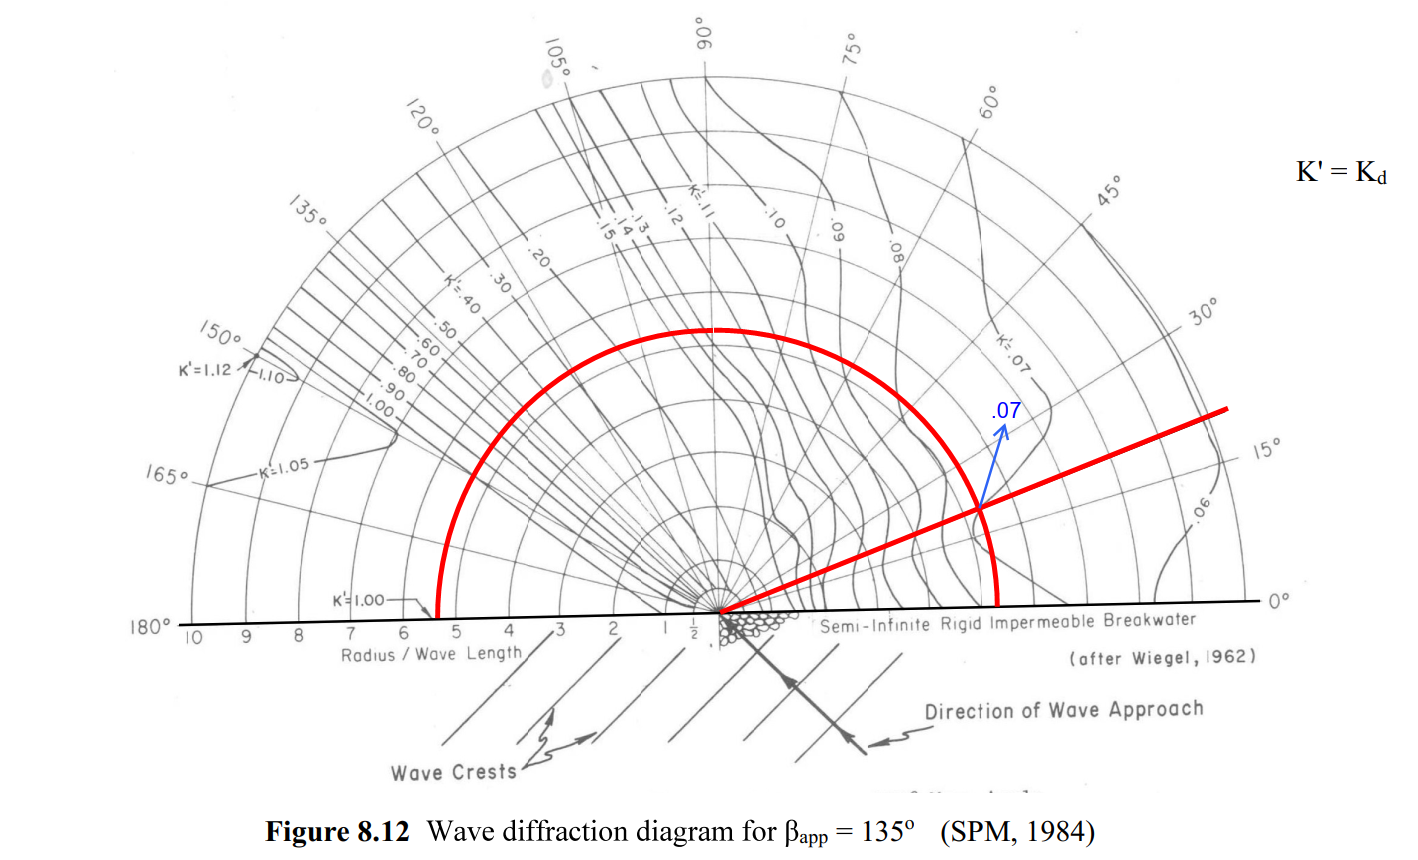
\includegraphics[width=0.8\textwidth]{diffraction_135.png}
    \caption{Diffraction coefficient reading for \(\beta_{app}=135^\circ\).}
    \label{fig:diffraction_135}
\end{figure}

\begin{figure}[H]
    \centering
    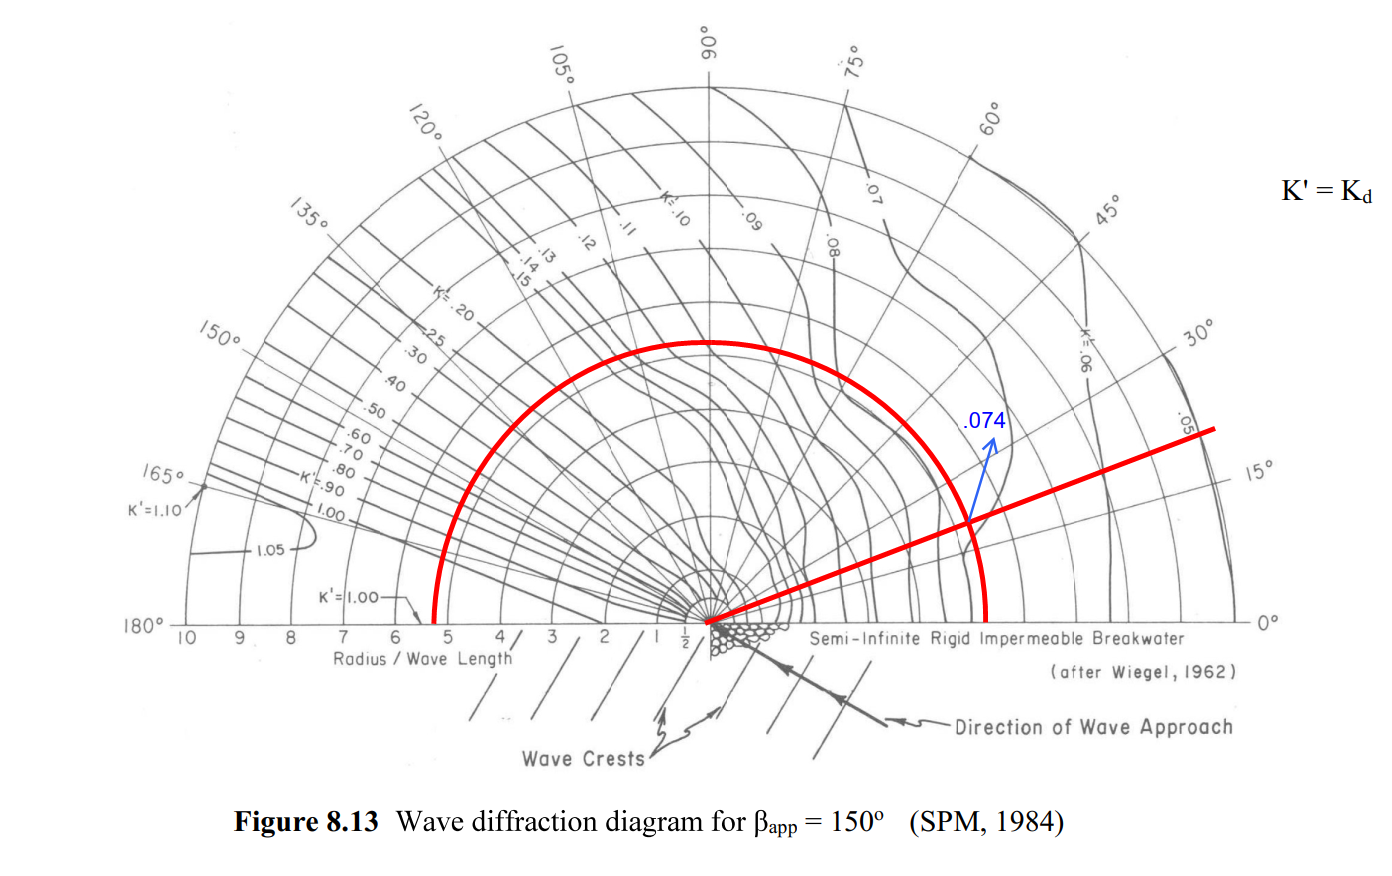
\includegraphics[width=0.8\textwidth]{diffraction_150.png}
    \caption{Diffraction coefficient reading for \(\beta_{app}=150^\circ\).}
    \label{fig:diffraction_150}
\end{figure}

The incident significant wave height at Section C-C was then calculated as

\begin{equation}
    H_i=K_d H_{head}=0.0724(2.80403)=0.2030~\mathrm{m}
\end{equation}

The maximum design wave height was then calculated as

\begin{equation}
    H_{max}=1.8H_i
\end{equation}

The wave period was taken as \(T=7.2016~\mathrm{s}\). The local wavelength was obtained from the linear dispersion relation:

\begin{equation}
    L=\frac{gT^2}{2\pi}\tanh\left(\frac{2\pi h}{L}\right)
\end{equation}

The allowable harbour agitation was taken as \(H_{t,allow}=0.30~\mathrm{m}\). Since the diffracted incident wave at Section C-C was already below this limit, no additional wave attenuation was required for the basic wave-height check. Therefore, the required transmission coefficient was taken as

\begin{equation}
    K_{t,req}=1.0
\end{equation}

and the transmitted wave height for the requirement check was calculated as

\begin{equation}
    H_t=K_{t,req}H_i
\end{equation}

The selected floating breakwater geometry was also checked using the Wiegel and Macagno transmission formulas. The Wiegel transmission coefficient was calculated as

\begin{equation}
    K_{t,Wie}=
    \sqrt{
    \frac{
    4\pi(h-h_d)/L+\sinh\left(4\pi(h-h_d)/L\right)
    }
    {
    \sinh(4\pi h/L)+4\pi h/L
    }}
\end{equation}

The Macagno transmission coefficient was calculated as

\begin{equation}
    K_{t,Mac}=
    \frac{1}
    {
    \sqrt{
    1+
    \left[
    \frac{\pi B_{fb}\sinh(kh)}
    {L\cosh\left(2\pi(h-h_d)/L\right)}
    \right]^2
    }}
\end{equation}

where \(k=2\pi/L\), \(B_{fb}\) is the floating breakwater width, and \(h_d\) is the draft.

Unlike the previous floating pier design, the width was not selected by iterating for a target \(K_t\). In this case, attenuation was not governing because the diffracted incident wave was already small. Therefore, the draft was selected from floating stability requirements, and the width was selected using the recommended ratio

\begin{equation}
    \frac{B_{fb}}{h_d}=3
\end{equation}

The freeboard was taken as \(h_f=0.80~\mathrm{m}\), and the total box height was calculated as

\begin{equation}
    h_{tot}=h_f+h_d
\end{equation}

\subsubsection{Draft Selection and Wall Thickness}

\hspace*{0.5cm} The draft was selected to satisfy the metacentric height and eccentric loading requirements. The basic metacentric height requirement was taken as

\begin{equation}
    GM_{req,basic}=0.20~\mathrm{m}
\end{equation}

The eccentric loading requirement was based on a live load of \(q=5.0~\mathrm{kN/m^2}\) applied to half of the floating breakwater width. With \(B_{fb}=3h_d\), the required metacentric height from eccentric loading was calculated as

\begin{equation}
    GM_{req,\phi}=
    \frac{q(B_{fb}/h_d)}
    {8\gamma_w\Phi_{lim}}
\end{equation}

where \(\Phi_{lim}=0.105~\mathrm{rad}\). The governing required metacentric height was taken as

\begin{equation}
    GM_{req}=\max(GM_{req,basic},GM_{req,\phi})
\end{equation}

Using \(B_{fb}/h_d=3\), the draft was obtained from

\begin{equation}
    h_d=
    \frac{12(GM_{req}+h_f/2)}
    {(B_{fb}/h_d)^2}
\end{equation}

The calculated draft was rounded up to the nearest \(0.10~\mathrm{m}\). The width was then calculated as

\begin{equation}
    B_{fb}=3h_d
\end{equation}

The wall thickness of the hollow concrete box was obtained from buoyancy equilibrium. The weight of the concrete box was set equal to the displaced water weight at the selected draft:

\begin{equation}
    \gamma_c\left[B_{fb}h_{tot}-(B_{fb}-2t)(h_{tot}-2t)\right]
    =
    \gamma_w B_{fb}h_d
\end{equation}

This equation was solved for the wall thickness \(t\).

\subsubsection{Floating Stability}

\hspace*{0.5cm} The floating stability checks were carried out after the draft and width were selected. The centre of buoyancy and centre of gravity were taken as

\begin{equation}
    B^*=\frac{h_d}{2}
\end{equation}

\begin{equation}
    G=\frac{h_{tot}}{2}
\end{equation}

The vertical distance between them was calculated as

\begin{equation}
    a=G-B^*
\end{equation}

The metacentric radius was calculated as

\begin{equation}
    \rho=\frac{B_{fb}^{2}}{12h_d}
\end{equation}

and the metacentric height was obtained from

\begin{equation}
    GM=\rho-a
\end{equation}

The basic stability requirement was

\begin{equation}
    GM\geq0.20~\mathrm{m}
\end{equation}

For the eccentric loading check, the live load was applied to half of the floating breakwater width:

\begin{equation}
    P_{ecc}=q\frac{B_{fb}}{2}
\end{equation}

The lever arm was taken as

\begin{equation}
    l=\frac{B_{fb}}{4}
\end{equation}

and the tilting moment was calculated as

\begin{equation}
    M_{tilt}=P_{ecc}l
\end{equation}

The resulting tilt angle was calculated as

\begin{equation}
    \Phi=
    \frac{M_{tilt}}
    {\gamma_w V_{sub}GM}
\end{equation}

where

\begin{equation}
    V_{sub}=B_{fb}h_d
\end{equation}

The eccentric loading criterion was

\begin{equation}
    \Phi\leq0.105~\mathrm{rad}
\end{equation}

The distributed loading stability condition was also checked using

\begin{equation}
    \frac{\gamma_w I}{W}-a>0
\end{equation}

where

\begin{equation}
    I=\frac{B_{fb}^{3}}{12}
\end{equation}

and

\begin{equation}
    W=\gamma_w B_{fb}h_d+qB_{fb}
\end{equation}

\subsubsection{Design Forces}

\hspace*{0.5cm} The design forces acting on the floating breakwater were calculated using the same force components used in the floating pier design. These include hydrostatic wave forces, wave drift force, drag and inertia forces, wind force, and current drag force.

For the rear-side wave force calculation, the transmitted maximum wave height was calculated using the Wiegel transmission coefficient of the selected geometry:

\begin{equation}
    H_{t,force}=K_{t,Wie}H_{max}
\end{equation}

The pressure intensities on the front face, rear face, and base were calculated as

\begin{equation}
    p_1=
    \begin{cases}
    (H_{max}-h_f)\gamma_w, & H_{max}\geq h_f \\
    0, & H_{max}<h_f
    \end{cases}
\end{equation}

\begin{equation}
    p_2=(H_{max}+h_d)\gamma_w
\end{equation}

\begin{equation}
    p_3=\left(h_d+\frac{H_{t,force}}{2}\right)\gamma_w
\end{equation}

\begin{equation}
    p_4=p_2-p_3
\end{equation}

The hydrostatic force on the front face was calculated as

\begin{equation}
    F_{hf}=\frac{(h_d+h_f)(p_1+p_2)}{2}
\end{equation}

The hydrostatic force on the rear face was calculated as

\begin{equation}
    F_{hr}=
    \frac{(h_d-H_{t,force}/2)p_3}{2}
\end{equation}

The uplift force was calculated as

\begin{equation}
    F_u=\frac{B_{fb}p_4}{2}
\end{equation}

The wave drift force was calculated as

\begin{equation}
    F_{wd}
    =
    \frac{1}{8}\gamma_w H_i^2K_r^2
    \left(
    1+
    \frac{4\pi h/L}{\sinh(4\pi h/L)}
    \right)
\end{equation}

where \(K_r=1.0\).

The orbital velocity and acceleration amplitudes were calculated as

\begin{equation}
    u_m=
    \frac{H_{max}}{2}
    \frac{gT}{L}
    \frac{
    \cosh\left(2\pi(H_{max}/2+h)/L\right)
    }
    {
    \cosh(2\pi h/L)
    }
\end{equation}

\begin{equation}
    a_x=
    \frac{H_{max}g\pi}{L}
    \frac{
    \cosh\left(2\pi(H_{max}/2+h)/L\right)
    }
    {
    \cosh(2\pi h/L)
    }
\end{equation}

The drag and inertia forces were calculated over one wave period as

\begin{equation}
    F_d=C_D h_d\rho_w\frac{u^2}{2}
\end{equation}

\begin{equation}
    F_i=C_M A_{sub}\rho_w a_x
\end{equation}

where

\begin{equation}
    A_{sub}=B_{fb}h_d
\end{equation}

The total orbital wave force was taken as the maximum value of

\begin{equation}
    F_t=F_d+F_i
\end{equation}

over one wave period.

The wind speed was taken as \(u_w=15.175~\mathrm{m/s}\), and the current speed was taken as

\begin{equation}
    u_c=0.02u_w
\end{equation}

The wind force was calculated as

\begin{equation}
    F_w=C_{DW}(2h_f)\rho_{air}\frac{u_w^2}{2}
\end{equation}

The current drag force was calculated as

\begin{equation}
    F_{cd}=C_{DC}h_d\rho_w\frac{u_c^2}{2}
\end{equation}

The total horizontal force used for the mooring design was calculated as

\begin{equation}
    P=(F_{hf}-F_{hr})+F_{wd}+F_{t,max}+F_w+F_{cd}
\end{equation}

\subsubsection{Mooring Line Design}

\hspace*{0.5cm} The wave-induced horizontal and vertical displacements were estimated from the water particle trajectory at the still water level. The horizontal displacement amplitude was calculated as

\begin{equation}
    A=
    \frac{H_{max}}{2}
    \frac{\cosh(2\pi h/L)}{\sinh(2\pi h/L)}
\end{equation}

and the vertical displacement amplitude was calculated as

\begin{equation}
    B=
    \frac{H_{max}}{2}
    \frac{\sinh(2\pi h/L)}{\sinh(2\pi h/L)}
\end{equation}

The mooring chain was designed to resist the total horizontal force \(P\). The water depth below the floating breakwater bottom was calculated as

\begin{equation}
    h_{moor}=h-h_d
\end{equation}

The submerged chain weight was taken as \(w=0.5~\mathrm{kN/m}\). The maximum projected chain length was calculated as

\begin{equation}
    L_{max}=\sqrt{\frac{2Ph_{moor}}{w}}
\end{equation}

The minimum projected chain length was calculated as

\begin{equation}
    L_{min}
    =
    -\frac{P\tan\alpha_B}{w}
    +
    \sqrt{
    \left(
    \frac{P\tan\alpha_B}{w}
    \right)^2
    +
    \frac{2Ph_{moor}}{w}
    }
\end{equation}

where \(\alpha_B=6^{\circ}\) was used as the limiting anchor angle. The projected chain length was taken as

\begin{equation}
    L_{proj}=L_{min}
\end{equation}

The pontoon-end and anchor-end chain angles were calculated as

\begin{equation}
    \theta_2=
    \tan^{-1}
    \left(
    \frac{h_{moor}}{L_{proj}}
    +
    \frac{wL_{proj}}{2P}
    \right)
\end{equation}

\begin{equation}
    \theta_1=
    \tan^{-1}
    \left(
    \frac{h_{moor}}{L_{proj}}
    -
    \frac{wL_{proj}}{2P}
    \right)
\end{equation}

The vertical forces at the anchor and pontoon were calculated as

\begin{equation}
    V_a=P\tan\theta_1
\end{equation}

\begin{equation}
    V_b=P\tan\theta_2
\end{equation}

The maximum chain tension was calculated as

\begin{equation}
    T_{max}=\frac{P}{\cos\theta_2}
\end{equation}

The chain sag was estimated as

\begin{equation}
    f=\frac{wL_{proj}^{2}}{8P}
\end{equation}

Finally, the catenary chain length was computed by numerical integration:

\begin{equation}
    S=
    \int_0^{L_{proj}}
    \sqrt{
    1+
    \left(
    \frac{dy}{dx}
    \right)^2
    }
    dx
\end{equation}

where

\begin{equation}
    \frac{dy}{dx}=
    \frac{V_a+wx}{P}
\end{equation}



% -------------------- Results and Discussion --------------------
\section{Results and Discussion}

\subsection{Rubble Mound Breakwater Design}

\hspace*{0.5cm} The rubble mound breakwater calculations were carried out for Sections A-A and B-B. Both sections were treated as trunk sections. The SWANOne \(H_{1/3}\) value was used as the design wave height in the armour stability equations, while \(H_{1/10}\) was used only in the Hudson check.

\begin{table}[H]
\centering
\caption{Hydraulic design basis for rubble mound breakwater calculations.}
\label{tab:rmbw_hydraulic}
\begin{tabular}{l c c}
\hline
Parameter & Section A-A & Section B-B \\
\hline
\(DWL_{HWL}\) (m MSL) & 1.2697 & 1.2697 \\
Design water depth, \(h\) (m) & 6.7697 & 13.2697 \\
SWAN \(H_{m0}\) at toe (m) & 2.8339 & 2.8148 \\
\(H_s\) used in equations, \(H_{1/3}\) (m) & 3.1109 & 2.8688 \\
\(T_p\) (s) & 7.2016 & 7.2016 \\
\(T_{m-1,0}\) (s) & 6.4599 & 6.5193 \\
\(H_{2\%}\) (m) & 4.3456 & 4.0074 \\
\(H_{1/10}\) (m) & 3.9545 & 3.6467 \\
\(\cot\alpha\) & 2 & 2 \\
\hline
\end{tabular}
\end{table}

The run-up results are close for the two sections, with Section A-A giving a slightly larger \(R_{u,2\%}\). The required crest elevation is also larger for A-A because the transformed design wave height is slightly larger at this section.

\begin{table}[H]
\centering
\caption{Run-up and crest height results for rubble mound alternatives.}
\label{tab:rmbw_runup_crest}
\begin{tabular}{l c c}
\hline
Parameter & Section A-A & Section B-B \\
\hline
\(\xi_{m-1,0}\) & 2.2882 & 2.4047 \\
\(R_{u,2\%}\) from Eq. 5.1 (m) & 4.9829 & 4.8291 \\
\(R_{u,2\%}\) from Eq. 5.2 (m) & 4.3633 & 4.1356 \\
Governing \(R_{u,2\%}\) (m) & 4.3633 & 4.1356 \\
Rock freeboard, \(R_c\) (m) & 4.3351 & 3.9477 \\
Rock crest elevation (m MSL) & 5.6048 & 5.2174 \\
X-Bloc freeboard, \(R_c\) (m) & 4.7686 & 4.3425 \\
X-Bloc crest elevation (m MSL) & 6.0383 & 5.6122 \\
X-Bloc \(R_c/H_s\) & 1.5329 & 1.5137 \\
\hline
\end{tabular}
\end{table}

The natural rock armour was checked using Hudson, Van der Meer (1988), Van der Meer (2021), and Van Gent (2003). In Section A-A, the relative water depth was \(h/H_s=2.1761<3\). Therefore, Van Gent (2003) was selected for the final armour sizing of Section A-A, following the Rock Manual recommendation for shallow toe conditions. In Section B-B, \(h/H_s=4.6256\), so Van der Meer (2021) was retained as the selected design method.

\begin{table}[H]
\centering
\caption{Natural rock armour stability results.}
\label{tab:rmbw_rock_methods}
\begin{tabular}{l c c c}
\hline
Method & Governing condition & Section A-A \(W\) (t) & Section B-B \(W\) (t) \\
\hline
Hudson & Non-breaking & 4.7827 & 3.7508 \\
Van der Meer (1988) & Plunging & 2.4718 & 2.0599 \\
Van der Meer (2021) & Plunging & 2.8188 & 2.3815 \\
Van Gent (3) & Plunging & 3.5436 & 2.9939 \\
\hline
Selected design method & -- & Van Gent (2003) & Van der Meer (2021) \\
Selected \(D_{n50}\) (m) & -- & 1.0949 & 0.9590 \\
Selected armour weight (t) & -- & 3.5436 & 2.3815 \\
\hline
\end{tabular}
\end{table}

\begin{table}[H]
\centering
\caption{Design method selection checks for natural rock armour.}
\label{tab:rmbw_method_selection}
\begin{tabular}{l c c c c}
\hline
\multirow{2}{*}{Criterion} & \multicolumn{2}{c}{Section A-A} & \multicolumn{2}{c}{Section B-B} \\
\cline{2-5}
 & Value & Status & Value & Status \\
\hline
\(h/H_s < 3\) & 2.1761 & YES & 4.6256 & NO \\
\(H_{2\%}/H_s < 1.4\) & 1.3969 & YES & 1.3969 & YES \\
\(H_s/H_{s0} < 0.9\) & 1.0133 & NO & 0.9345 & NO \\
\hline
Selected method & \multicolumn{2}{c}{Van Gent (2003)} & \multicolumn{2}{c}{Van der Meer (2021)} \\
Reason & \multicolumn{2}{c}{\(h/H_s<3\)} & \multicolumn{2}{c}{Deep-water toe condition} \\
\hline
\end{tabular}
\end{table}

The selected natural rock armour weight for Section A-A increased from the Van der Meer (2021) value to the Van Gent (2003) value because the section has a shallow toe condition. Therefore, the final armour weight for Section A-A became \(3.5436~\mathrm{t}\), with \(D_{n50}=1.0949~\mathrm{m}\). For Section B-B, the selected armour weight remained \(2.3815~\mathrm{t}\), with \(D_{n50}=0.9590~\mathrm{m}\).

\begin{table}[H]
\centering
\caption{Natural rock cross-section dimensions.}
\label{tab:rmbw_rock_section}
\begin{tabular}{l c c}
\hline
Parameter & Section A-A & Section B-B \\
\hline
Selected armour method & Van Gent (2003) & VdM (2021) \\
Armour weight, \(W_{design}\) (t) & 3.5436 & 2.3815 \\
Armour \(D_{n50}\) (m) & 1.0949 & 0.9590 \\
Armour layer thickness (m) & 2.1897 & 1.9180 \\
Underlayer \(D_{n50}\) (m) & 0.4977 & 0.4359 \\
Underlayer weight (t) & 0.3328 & 0.2237 \\
Underlayer thickness (m) & 0.9953 & 0.8718 \\
Crest width (m) & 3.2846 & 2.8771 \\
Crest elevation (m MSL) & 5.6048 & 5.2174 \\
Toe \(D_{n50}\) (m) & 0.5932 & 0.5470 \\
Toe weight (t) & 0.5635 & 0.4419 \\
Toe thickness (m) & 2.3727 & 2.1880 \\
Toe length (m) & 3.5590 & 3.2820 \\
Toe elevation (m MSL) & -2.7921 & -6.6921 \\
\hline
\end{tabular}
\end{table}

For the X-Bloc alternative, both sections initially required a corrected volume smaller than \(1.0~\mathrm{m^3}\). In Section A-A, the standard \(1.0~\mathrm{m^3}\) block also satisfied the row check. In Section B-B, the same initial block size failed the 20-row limit because of the larger water depth and longer slope length. Therefore, the X-Bloc size for B-B was increased to \(5.0~\mathrm{m^3}\).

\begin{table}[H]
\centering
\caption{X-Bloc design results.}
\label{tab:rmbw_xbloc}
\begin{tabular}{l c c}
\hline
Parameter & Section A-A & Section B-B \\
\hline
\(\Delta_x\) & 1.3301 & 1.3301 \\
Base unit volume, \(V_{base}\) (m\(^3\)) & 0.4550 & 0.4459 \\
Depth correction factor, \(CF\) & 2 & 2 \\
Corrected volume, \(V_{CF}\) (m\(^3\)) & 0.9101 & 0.8919 \\
Initial standard volume (m\(^3\)) & 1 & 1 \\
Rows with initial block & 15.8434 & 31.8153 \\
Initial row check & PASS & FAIL \\
Final X-Bloc volume (m\(^3\)) & 1 & 5 \\
X-Bloc unit weight (t) & 2.4 & 12 \\
Unit height, \(D\) (m) & 1.44 & 2.47 \\
Upslope placement distance, \(D_y\) (m) & 0.91 & 1.55 \\
Final number of rows & 15.8434 & 18.3464 \\
X-Bloc crest elevation (m MSL) & 6.0383 & 5.6122 \\
Underlayer \(W_{50}\) (t) & 0.34 & 1.7 \\
Underlayer \(D_{n50}\) (m) & 0.5012 & 0.8571 \\
Underlayer thickness (m) & 1.0025 & 1.7142 \\
Toe \(D_{n50}\) (m) & 0.5012 & 0.8571 \\
Toe weight (t) & 0.34 & 1.7 \\
Toe thickness (m) & 1.0025 & 1.7142 \\
Toe length (m) & 1.5037 & 2.5713 \\
\hline
\end{tabular}
\end{table}

Overall, both natural rock and X-Bloc alternatives are hydraulically feasible for the rubble mound design. The natural rock alternative gives smaller unit weights and lower crest levels. The rear side was not designed separately because the crest level was based on a strict allowable overtopping discharge of \(q=1~\mathrm{L/s/m}\). This limits the loading expected behind the crest. Therefore, the rear side was taken symmetrical in the cross-section drawings to stay on the safe side.

\subsection{Berm Breakwater Design}

\hspace*{0.5cm} The berm breakwater calculations were carried out for Sections A-A and B-B under the HWL condition. The actual SWANOne wave height at each section was used in the calculations, while \(H_{sD}=3.0~\mathrm{m}\) was used as the reference value for the preliminary rock class check. For B-B, the Class I armour was selected from the lecture-table representative rock class. For A-A, the relative water depth was \(h/H_s=2.1761<3\), so the Class I armour size was governed by the Van Gent shallow-water formulation. The A-A slope was therefore taken as \(\cot\alpha=2.0\), which satisfies the validity range of the Van Gent method. A two-class rock section was adopted, with Class I armour on the berm and Class II rock for the lower layer and toe.

\begin{table}[H]
\centering
\caption{Governing hydraulic conditions for berm breakwater design.}
\label{tab:berm_hydraulic}
\begin{tabular}{l c c}
\hline
Parameter & Section A-A & Section B-B \\
\hline
\(DWL_{HWL}\) (m MSL) & 1.2697 & 1.2697 \\
\(h_{NWL}\) (m) & 5.5 & 12.0 \\
Water depth at DWL, \(h\) (m) & 6.7697 & 13.2697 \\
Actual \(H_{sD}\) (m) & 2.8339 & 2.8148 \\
Table \(H_{sD}\) (m) & 3 & 3 \\
Overload wave height, \(H_{sOL}\) (m) & 3.4006 & 3.3778 \\
\(T_p\) (s) & 7.2016 & 7.2016 \\
MHWS (m MSL) & 0.2 & 0.2 \\
Construction margin, \(\Delta_w\) (m) & 1 & 1 \\
Design slope, \(\cot\alpha_d\) & 2 & 1.5 \\
\hline
\end{tabular}
\end{table}

For Section A-A, the Van Gent shallow-water validity checks were satisfied. Therefore, the Van Gent armour size was accepted as the governing Class I armour size for this section. For Section B-B, the section remained within the deep-toe/conservative range, so the lecture-table representative Class I rock was used.

\begin{table}[H]
\centering
\caption{Class I armour rock selection and berm classification.}
\label{tab:berm_classI}
\begin{tabular}{l c c}
\hline
Parameter & Section A-A & Section B-B \\
\hline
Selected armour class & Class I: 1--4 t & Class I: 1--4 t \\
Sizing source & Van Gent shallow-water sizing & Lecture-table representative rock \\
\(M_{50,I}\) (t) & 3.5436 & 2.5 \\
\(D_{n50,I}\) (m) & 1.0949 & 0.9747 \\
\(\Delta\) & 1.6341 & 1.6341 \\
\(N_s\) using \(H_{sD}=3.0~\mathrm{m}\) & 1.6768 & 1.8835 \\
\(N_s\) using actual \(H_{sD}\) & 1.5839 & 1.7673 \\
Berm type & More stable than HR-IC range & HR-IC \\
15 t check & YES & YES \\
\hline
\end{tabular}
\end{table}

The recession was calculated for both the design and overload wave conditions. The accepted resiliency was taken as \(P=20\%\). The selected berm width was governed by the resiliency criterion in both sections.

\begin{table}[H]
\centering
\caption{Recession and berm width results.}
\label{tab:berm_recession_width}
\begin{tabular}{l c c}
\hline
Parameter & Section A-A & Section B-B \\
\hline
Design recession, \(Rec_{ND}\) (m) & 0.4564 & 0.8042 \\
Overload recession, \(Rec_{OL}\) (m) & 1.3487 & 2.0736 \\
Design recession, \(Rec_{design}\) (m) & 0.9025 & 1.4389 \\
Resiliency, \(P\) (\%) & 20 & 20 \\
Berm width from resiliency (m) & 4.5127 & 7.1943 \\
Minimum berm width (m) & 3.2846 & 2.9240 \\
Selected berm width, \(B\) (m) & 4.5127 & 7.1943 \\
\hline
\end{tabular}
\end{table}

The horizontal armour width and berm level were calculated using the selected Class I armour size. In both sections, the berm depth was governed by the construction margin and the armour thickness, rather than by \(0.6H_{sD}\). The resulting berm elevation is higher in A-A because the Van Gent sizing gives a larger Class I armour diameter. The validity checks showed that \(d_b/H_{sD}\) was above 0.6 for both sections.

\begin{table}[H]
\centering
\caption{Berm level and transition results.}
\label{tab:berm_level_transition}
\begin{tabular}{l c c}
\hline
Parameter & Section A-A & Section B-B \\
\hline
Horizontal armour width, \(A_h\) (m) & 8.9772 & 9.9490 \\
\(A_h/H_{sD}\) & 3.1678 & 3.5345 \\
\(0.6H_{sD}\) (m) & 1.7003 & 1.6889 \\
\(\Delta_w+2D_{n50,I}\) (m) & 3.1897 & 2.9493 \\
Governing \(d_b\) above MHWS (m) & 3.1897 & 2.9493 \\
\(d_b/H_{sD}\) & 1.1256 & 1.0478 \\
Berm elevation (m MSL) & 3.3897 & 3.1493 \\
Berm above DWL (m) & 2.1200 & 1.8796 \\
Transition depth, \(h_{I-II}\) below NWL (m) & 3.3100 & 2.9466 \\
\hline
\end{tabular}
\end{table}

Class II rock was selected for the lower layer and toe. A separate Class III layer was not included because the simplified two-class section was sufficient for this preliminary design.

\begin{table}[H]
\centering
\caption{Lower rock class selection.}
\label{tab:berm_lower_class}
\begin{tabular}{l c c}
\hline
Parameter & Section A-A & Section B-B \\
\hline
Selected lower class & Class II: 0.2--1 t & Class II: 0.2--1 t \\
\(M_{50,II}\) (t) & 0.4472 & 0.4472 \\
\(D_{n50,II}\) (m) & 0.5492 & 0.5492 \\
\(N_s\) if exposed to \(H_{sD}\) & 3.1577 & 3.1365 \\
\hline
\end{tabular}
\end{table}

The crest level was checked for both the design and overload conditions. In both sections, the design condition with \(q=1~\mathrm{L/s/m}\) governed over the overload condition with \(q=10~\mathrm{L/s/m}\).

\begin{table}[H]
\centering
\caption{Crest height results for berm breakwater design.}
\label{tab:berm_crest}
\begin{tabular}{l c c}
\hline
Parameter & Section A-A & Section B-B \\
\hline
\(\gamma_{BB}\), design condition & 0.4429 & 0.3958 \\
Design \(R_c\) (m) & 3.8217 & 3.3885 \\
Overload \(R_c\) (m) & 3.4093 & 3.0718 \\
Governing \(R_c\) (m) & 3.8217 & 3.3885 \\
Crest elevation, \(z_{crest}\) (m MSL) & 5.0914 & 4.6582 \\
Crest width (m) & 2.1967 & 2.1967 \\
\(R_c/H_{sD}\), design condition & 1.3486 & 1.2038 \\
\hline
\end{tabular}
\end{table}

The toe berm was designed using Class II rock. The overload condition governed the toe elevation in both sections. The calculated toe geometry satisfied the validity limits for \(h_t/h\) and \(h_t/D_{n50}\), and the toe was constructable in both cases.

\begin{table}[H]
\centering
\caption{Toe berm design results.}
\label{tab:berm_toe}
\begin{tabular}{l c c}
\hline
Parameter & Section A-A & Section B-B \\
\hline
Toe rock class & Class II & Class II \\
Toe \(D_{n50}\) (m) & 0.5492 & 0.5492 \\
Toe \(M_{50}\) (t) & 0.4472 & 0.4472 \\
Design toe elevation (m MSL) & -2.2715 & -5.6219 \\
Design \(h_t\) (m) & 3.5412 & 6.8916 \\
\(h_t/h\) & 0.5231 & 0.5193 \\
\(h_t/D_{n50}\) & 6.4481 & 12.5488 \\
Constructable & YES & YES \\
\hline
\end{tabular}
\end{table}

Overall, the berm breakwater alternative gives feasible results for both A-A and B-B. Section A-A is controlled by shallow-water armour sizing and requires a \(3.5436~\mathrm{t}\) primary armour stone. Section B-B remains an HR-IC berm breakwater with a \(2.5~\mathrm{t}\) primary armour stone, but it requires a wider berm and a deeper toe because of the larger local water depth.


\subsection{Vertical Wall Breakwater Design}

\hspace*{0.5cm} The composite vertical wall alternative was checked for Sections A-A and B-B under the HWL condition. The SWANOne wave parameters at the toe were used as the hydraulic input. The design wave height for the Goda/Takahashi pressure calculation was taken as \(H_{design}=H_{max}=5.0618~\mathrm{m}\) for both sections. The wall width was optimized by checking different rubble mound foundation geometries and then rounded up to the nearest \(0.1~\mathrm{m}\).

\begin{table}[H]
\centering
\caption{Hydraulic design basis for vertical wall breakwater calculations.}
\label{tab:vertical_hydraulic}
\begin{tabular}{l c c}
\hline
Parameter & Section A-A & Section B-B \\
\hline
\(DWL_{HWL}\) (m MSL) & 1.2697 & 1.2697 \\
\(h_{NWL}\) (m) & 5.5 & 12.0 \\
Design water depth, \(h_s\) (m) & 6.9508 & 13.2544 \\
SWAN \(X_P\) (m) & 159.0 & 122.0 \\
\(H_{m0}\) at toe (m) & 2.8223 & 2.8286 \\
\(H_{1/3}\) at toe (m) & 3.0162 & 2.8667 \\
\(H_{2\%}\) at toe (m) & 4.2132 & 4.0045 \\
\(H_{1/10}\) at toe (m) & 3.8341 & 3.6441 \\
\(T_p\) at toe (s) & 7.2016 & 7.2016 \\
\(T_{m01}\) at toe (s) & 6.0249 & 6.0071 \\
\(T_{m-1,0}\) at toe (s) & 6.5566 & 6.5090 \\
Local wavelength, \(L\) (m) & 49.2657 & 60.9450 \\
\(H_{max}\) (m) & 5.0618 & 5.0618 \\
\(H_{design}\) (m) & 5.0618 & 5.0618 \\
Allowable overtopping, \(q\) (L/s/m) & 1.0 & 1.0 \\
\hline
\end{tabular}
\end{table}

The optimized composite sections are summarized in Table~\ref{tab:vertical_geometry}. Section B-B required a deeper rubble mound foundation because of the larger local water depth. The final rounded wall width was \(5.4~\mathrm{m}\) for A-A and \(5.7~\mathrm{m}\) for B-B.

\begin{table}[H]
\centering
\caption{Optimized composite vertical wall geometry.}
\label{tab:vertical_geometry}
\begin{tabular}{l c c}
\hline
Parameter & Section A-A & Section B-B \\
\hline
\(h_1/h_s\) & 0.80 & 0.71 \\
Rubble mound height below DWL, \(h_1\) (m) & 5.5606 & 9.4106 \\
\(B_m/h_s\) & 0.30 & 0.30 \\
Rubble mound width, \(B_m\) (m) & 2.0852 & 3.9763 \\
Depth above mound, \(d\) (m) & 4.5853 & 8.2880 \\
Wall-bottom depth below DWL, \(h'\) (m) & 5.5606 & 9.4106 \\
Mound armour \(D_{n50}\) (m) & 0.4877 & 0.5613 \\
Mound armour \(M_{50}\) (t) & 0.3131 & 0.4774 \\
Wall freeboard, \(h_c\) (m) & 6.3364 & 6.3364 \\
Exact wall width (m) & 5.3953 & 5.6702 \\
Rounded wall width (m) & 5.40 & 5.70 \\
\hline
\end{tabular}
\end{table}

The Goda/Takahashi pressure coefficients and resulting pressures are given in Tables~\ref{tab:vertical_coefficients} and~\ref{tab:vertical_pressures}. Section A-A produced higher pressure values because the shallower depth led to larger pressure coefficients. In Section B-B, the pressure values were lower, but the total moment was larger because the pressure acted over a greater structural height.

\begin{table}[H]
\centering
\caption{Goda/Takahashi pressure coefficients.}
\label{tab:vertical_coefficients}
\begin{tabular}{l c c}
\hline
Parameter & Section A-A & Section B-B \\
\hline
\(\eta^*\) (m) & 7.5927 & 7.5927 \\
\(\alpha_1\) & 0.7923 & 0.6637 \\
\(\alpha_2\) & 0.2068 & 0.0585 \\
\(\alpha_3\) & 0.7636 & 0.6300 \\
\(\alpha_I\) & 0.1282 & 0.1269 \\
\(\alpha^*\) & 0.2068 & 0.1269 \\
\hline
\end{tabular}
\end{table}

\begin{table}[H]
\centering
\caption{Wave pressure results for vertical wall design.}
\label{tab:vertical_pressures}
\begin{tabular}{l c c}
\hline
Pressure component & Section A-A & Section B-B \\
\hline
\(p_1\) (kPa) & 50.8504 & 40.2420 \\
\(p_2\) (kPa) & 8.4140 & 6.6587 \\
\(p_3\) (kPa) & 38.8315 & 25.3524 \\
\(p_u\) (kPa) & 30.7931 & 21.2820 \\
\hline
\end{tabular}
\end{table}

The calculated horizontal forces, overturning moments, and factors of safety are shown in Table~\ref{tab:vertical_stability}. Both sections satisfied the required stability criterion. The rounded wall widths gave sliding and overturning safety factors larger than 1.2 for both A-A and B-B.

\begin{table}[H]
\centering
\caption{Forces and stability results for vertical wall design.}
\label{tab:vertical_stability}
\begin{tabular}{l c c}
\hline
Parameter & Section A-A & Section B-B \\
\hline
Horizontal force, \(F_H\) (kN/m) & 437.1054 & 457.2327 \\
Overturning moment, \(M_{FH}\) (kN.m/m) & 2221.1775 & 3318.8733 \\
Sliding FS & 1.5477 & 1.9857 \\
Overturning FS & 1.3369 & 1.2821 \\
\hline
\end{tabular}
\end{table}

The vertical wall alternative is structurally feasible for both sections based on sliding and overturning checks. In Section A-A, the pressures are larger because of the shallower water depth, but the smaller pressure height keeps the total overturning moment lower. In Section B-B, the deeper section increases the moment arm and produces a larger overturning moment.


\subsection{Floating Breakwater Design}

\hspace*{0.5cm} Section C-C was designed as a floating breakwater under the HWL condition. The wave height at the breakwater head was first reduced using the diffraction coefficient \(K_d=0.0724\). This gave an incident wave height of \(H_i=0.2030~\mathrm{m}\) at Section C-C. Since this value was already smaller than the allowable transmitted wave height of \(0.30~\mathrm{m}\), wave attenuation was not the governing design criterion. The final dimensions were mainly controlled by floating stability under eccentric loading.

\begin{table}[H]
\centering
\caption{Hydraulic design basis for Section C-C floating breakwater.}
\label{tab:floating_hydraulic}
\begin{tabular}{l c}
\hline
Parameter & Value \\
\hline
\(DWL_{HWL}\) (m MSL) & 1.2697 \\
\(h_{NWL}\) (m) & 4.0 \\
Design water depth, \(h\) (m) & 5.2697 \\
Wave height at breakwater head, \(H_{head}\) (m) & 2.8040 \\
Diffraction coefficient, \(K_d\) & 0.0724 \\
Incident wave height at C-C, \(H_i\) (m) & 0.2030 \\
Maximum wave height, \(H_{max}\) (m) & 0.3654 \\
Wave period, \(T\) (s) & 7.2016 \\
Local wavelength, \(L\) (m) & 48.2354 \\
Wave number, \(k\) (rad/m) & 0.13026 \\
Allowable transmitted wave height, \(H_{t,allow}\) (m) & 0.30 \\
Required-check \(K_t\) & 1.0 \\
Required-check transmitted height, \(H_t\) (m) & 0.2030 \\
\(H_t \leq H_{t,allow}\) & YES \\
\hline
\end{tabular}
\end{table}

The selected floating breakwater geometry is summarized in Table~\ref{tab:floating_geometry}. The draft was selected from the stability requirement, while the width was taken as \(B_{fb}/h_d=3.0\). This ratio is within the recommended range of 2 to 3. The value of \(L/B_{fb}=5.54\) exceeds the recommended limit for effective attenuation, but this was not critical because the diffracted incident wave height was already below the harbour agitation limit.

\begin{table}[H]
\centering
\caption{Selected floating breakwater geometry.}
\label{tab:floating_geometry}
\begin{tabular}{l c}
\hline
Parameter & Value \\
\hline
Freeboard, \(h_f\) (m) & 0.8\\
Draft, \(h_d\) (m) & 2.9 \\
Total height, \(h_{tot}\) (m) & 3.7 \\
Floating breakwater width, \(B_{fb}\) (m) & 8.7 \\
\(B_{fb}/h_d\) & 3.0 \\
\(L/B_{fb}\) & 5.5443 \\
Wall thickness, \(t\) (m) & 0.4801 \\
\hline
\end{tabular}
\end{table}

The selected geometry was checked using the Wiegel and Macagno transmission formulations. Both formulas gave transmitted wave heights below \(0.30~\mathrm{m}\), confirming that the selected section satisfies the wave transmission requirement.

\begin{table}[H]
\centering
\caption{Wave transmission checks for the selected floating breakwater geometry.}
\label{tab:floating_transmission}
\begin{tabular}{l c c}
\hline
Method & \(K_t\) & \(H_t\) (m) \\
\hline
Required check & 1.0 & 0.2030 \\
Wiegel & 0.6292 & 0.1277 \\
Macagno & 0.9282 & 0.1884 \\
\hline
Allowable \(H_t\) (m) & \multicolumn{2}{c}{0.30} \\
\hline
\end{tabular}
\end{table}

The floating stability results are given in Table~\ref{tab:floating_stability}. The required metacentric height was controlled by the eccentric loading criterion, not by the basic \(GM\) limit. The final geometry gave \(GM=1.7750~\mathrm{m}\), which is slightly above the adopted required value of \(1.7422~\mathrm{m}\). The resulting tilt angle was \(0.10306~\mathrm{rad}\), which satisfies the limit of \(0.105~\mathrm{rad}\).

\begin{table}[H]
\centering
\caption{Floating stability results.}
\label{tab:floating_stability}
\begin{tabular}{l c}
\hline
Parameter & Value \\
\hline
Basic required \(GM\) (m) & 0.20 \\
Required \(GM\) from eccentric loading (m) & 1.7422 \\
Adopted required \(GM\) (m) & 1.7422 \\
\(B^*\) (m) & 1.45 \\
\(G\) from keel (m) & 1.85 \\
\(a\) (m) & 0.40 \\
\(\rho\) (m) & 2.1750 \\
Calculated \(GM\) (m) & 1.7750 \\
Live load, \(q_{live}\) (kN/m\(^2\)) & 5.00 \\
Eccentric load, \(P_{ecc}\) (kN/m) & 21.75 \\
Tilting moment, \(M_{tilt}\) (kN.m/m) & 47.3062 \\
Tilt angle, \(\Phi\) (rad) & 0.10306 \\
\(\Phi \leq 0.105~\mathrm{rad}\) & YES \\
Distributed loading stability term (m) & 1.4618 \\
Distributed loading stability check ($>0$) & PASS \\
\hline
\end{tabular}
\end{table}

The force components used for the mooring design are summarized in Table~\ref{tab:floating_forces}. The total horizontal design force was calculated as \(P=28.8921~\mathrm{kN/m}\). The largest additional dynamic component came from wave inertia, while wave drift, wind, and current forces were relatively small.

\begin{table}[H]
\centering
\caption{Horizontal force components for Section C-C floating breakwater.}
\label{tab:floating_forces}
\begin{tabular}{l c}
\hline
Parameter & Value \\
\hline
\(H_{t,force}=K_{t,Wiegel}H_{max}\) (m) & 0.2299 \\
Front hydrostatic force, \(F_{hf}\) (kN/m) & 61.9205 \\
Rear hydrostatic force, \(F_{hr}\) (kN/m) & 43.0335 \\
Uplift force, \(F_u\) (kN/m) & 11.1672 \\
Wave drift force, \(F_{wd}\) (kN/m) & 0.0921 \\
Submerged area, \(A_{sub}\) (m\(^2\)/m) & 25.23 \\
Maximum drag force, \(F_{d,max}\) (kN/m) & 0.2191 \\
Maximum inertia force, \(F_{i,max}\) (kN/m) & 9.1879 \\
Maximum wave drag and inertia force, \(F_{t,max}\) (kN/m) & 9.1879 \\
Wind force, \(F_w\) (kN/m) & 0.4514 \\
Current force, \(F_{cd}\) (kN/m) & 0.2738 \\
Total horizontal force, \(P\) (kN/m) & 28.8921 \\
\hline
\end{tabular}
\end{table}

The calculated floating body wave displacements were \(0.3067~\mathrm{m}\) horizontally and \(0.1827~\mathrm{m}\) vertically. These values were used as indicative motion amplitudes for the selected floating body.

\begin{table}[H]
\centering
\caption{Floating body wave displacement results.}
\label{tab:floating_displacements}
\begin{tabular}{l c}
\hline
Parameter & Value \\
\hline
Horizontal displacement amplitude, \(A\) (m) & 0.3067 \\
Vertical displacement amplitude, \(B\) (m) & 0.1827 \\
\hline
\end{tabular}
\end{table}

The mooring line was designed using the total horizontal force. The selected projected mooring length was \(11.5547~\mathrm{m}\), with a calculated chain length of \(11.8133~\mathrm{m}\). The maximum line tension was \(30.2066~\mathrm{kN/m}\).

\begin{table}[H]
\centering
\caption{Mooring line design results for Section C-C.}
\label{tab:floating_mooring}
\begin{tabular}{l c}
\hline
Parameter & Value \\
\hline
Mooring water depth, \(h_{moor}\) (m) & 2.3697 \\
Maximum projected length, \(L_{max}\) (m) & 16.5488 \\
Minimum projected length, \(L_{min}\) (m) & 11.5547 \\
Selected projected length, \(L_{proj}\) (m) & 11.5547 \\
Anchor angle (deg) & 6.0000 \\
Pontoon angle (deg) & 16.9652 \\
Anchor vertical reaction, \(V_a\) (kN/m) & 3.0367 \\
Pontoon vertical reaction, \(V_b\) (kN/m) & 8.8140 \\
Maximum line tension, \(T_{max}\) (kN/m) & 30.2066 \\
Sag, \(f\) (m) & 0.2888 \\
Chain length, \(S\) (m) & 11.8133 \\
\hline
\end{tabular}
\end{table}

Overall, the selected floating breakwater satisfies the wave transmission, buoyancy, floating stability, and mooring checks for Section C-C. The transmitted wave height remains below the allowable \(0.30~\mathrm{m}\) limit even with \(K_t=1.0\), and both the Wiegel and Macagno checks give smaller transmitted wave heights. The governing aspect of the design is the stability requirement under eccentric loading, which controls the selected draft and width.

The floating breakwater alternative was also checked for Sections A-A and B-B. However, these sections are directly exposed to the transformed design waves, with incident wave heights of \(3.1109~\mathrm{m}\) for A-A and \(2.8688~\mathrm{m}\) for B-B. These values are much larger than the usual practical wave-height range for floating breakwaters, which is about \(1.0\) to \(1.2~\mathrm{m}\). The wave period was also \(T=7.2016~\mathrm{s}\), which is longer than the typical \(4\) to \(5~\mathrm{s}\) range generally recommended for floating breakwater applications.

The harbour agitation limit was taken as \(H_{t,allow}=0.30~\mathrm{m}\). Therefore, the required transmission coefficients would be \(K_t=0.0964\) for A-A and \(K_t=0.1046\) for B-B. These values are very small for a floating breakwater. A Macagno transmission screening showed that satisfying these values would require impractically large floating dimensions. Therefore, the floating breakwater was not carried forward as a feasible alternative for Sections A-A and B-B.


\subsection{Structure Type Selection and Final Designs}

\subsubsection{Section A-A}

\hspace*{0.5cm} For Section A-A, the selected structure type was the conventional natural rock rubble mound breakwater. The final cross-section is shown in Figure~\ref{fig:rubble_AA}. This selection was made after comparing the natural rock rubble mound, X-Bloc armour alternative, Icelandic-type berm breakwater, and composite vertical wall alternative.

The first important point for Section A-A is the shallow-water condition. The ratio \(h/H_{s,toe}\) was smaller than 3, so the Van Gent (2003) shallow-water formulation was used for the natural rock armour sizing. This gave a required armour weight of \(3.5436~\mathrm{t}\) and a nominal diameter of \(D_{n50}=1.0949~\mathrm{m}\). Therefore, the final rubble mound section was not based on the smaller Van der Meer value, but on the more suitable shallow-water design approach.

The X-Bloc alternative was technically possible for A-A, since the row check was satisfied with a \(1.0~\mathrm{m^3}\) unit. However, it required special concrete armour units and a higher crest elevation than the natural rock rubble mound. The X-Bloc unit also had a larger characteristic block dimension, with \(D=1.44~\mathrm{m}\), and did not provide a clear dimensional advantage for this section. Since natural rock was already feasible with a practical armour size, the use of special concrete armour was not considered necessary.

The berm breakwater was also calculated using the same shallow-water logic. After this correction, the berm required the same primary armour size as the rubble mound, \(W=3.5436~\mathrm{t}\). Its crest elevation was lower than the rubble mound. However, this saving was not large enough to justify the additional complexity of an Icelandic-type berm section. The A-A berm also became more stable than the usual HR-IC range, meaning that it was not taking strong advantage of reshaping behaviour. In practice, it behaved more like a conservative bermed rubble mound rather than a clearly beneficial reshaping berm.

The composite vertical wall alternative was also stable for A-A. The rounded wall width was \(5.4~\mathrm{m}\), with safety factors of 1.5477 for sliding and 1.3369 for overturning. This makes the vertical wall much more compact than the rubble mound. However, Section A-A is relatively shallow, so this compactness is not essential unless there is a strict space limitation. The vertical wall would also require a larger concrete body, formwork or precasting, careful foundation preparation, and would produce more wave reflection. For a shallower section, the dissipative behaviour and construction ease of a rubble mound are more suitable.

For these reasons, the conventional natural rock rubble mound was selected for Section A-A. It uses a standard cross-section, avoids the special construction requirements of the berm and X-Bloc options, and avoids the cost and reflection issues associated with a vertical wall. Although it is not the most compact alternative, it is the most reasonable choice for the shallow A-A section when performance, constructability, and reliability are considered together.

\begin{figure}[H]
    \centering
    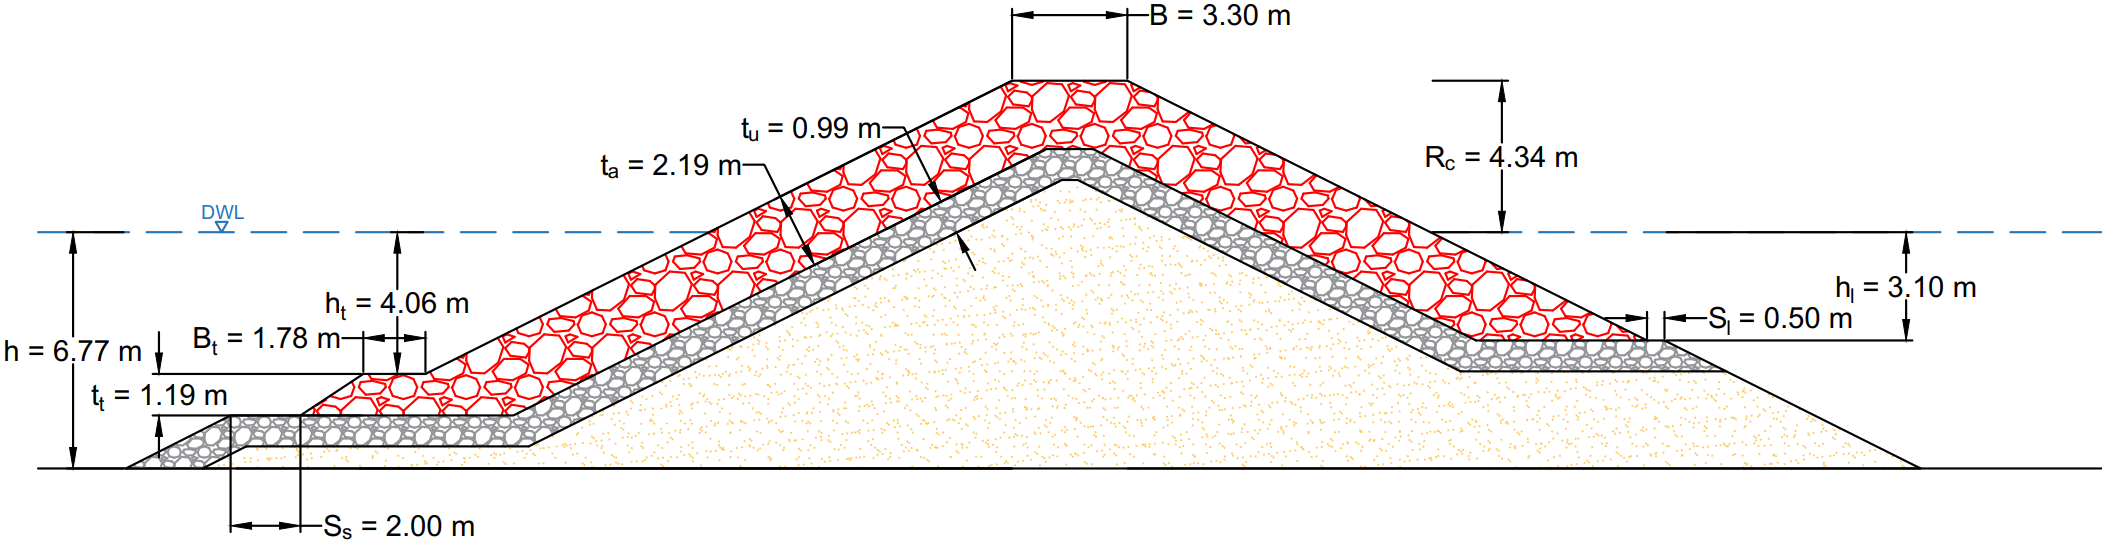
\includegraphics[width=0.95\textwidth]{Rubble_A.png}
    \caption{Selected natural rock rubble mound cross-section for Section A-A.}
    \label{fig:rubble_AA}
\end{figure}


\subsubsection{Section B-B}

\hspace*{0.5cm} For Section B-B, the selected structure type was the conventional natural rock rubble mound breakwater. However, the composite vertical wall was also considered in detail because B-B is the deeper section and the rubble mound footprint becomes large. Therefore, both the selected rubble mound cross-section and the vertical wall alternative are shown in this section.

The natural rock rubble mound was selected because it provides a standard breakwater section for marina conditions. The selected armour weight was \(2.3815~\mathrm{t}\), with \(D_{n50}=0.9590~\mathrm{m}\), based on the Van der Meer (2021) design method. The section has a crest elevation of \(5.2174~\mathrm{m}\) MSL and uses conventional armour, underlayer, core, and toe details. Although the total cross-section width is large, most of the inner volume consists of core material, which is less expensive and easier to place than concrete armour units or a massive vertical wall.

The X-Bloc alternative was less attractive for B-B. Although the corrected unit volume was initially below \(1.0~\mathrm{m^3}\), the row check failed because of the deeper water depth and longer slope length. As a result, the unit size had to be increased to \(5.0~\mathrm{m^3}\), corresponding to a \(12.0~\mathrm{t}\) concrete armour unit. This made the X-Bloc option less practical for this section, especially since it did not provide a crest elevation advantage over the natural rock alternative.

The berm breakwater was technically feasible for B-B and remained within the HR-IC range. It also gave a lower crest elevation than the rubble mound, \(4.6582~\mathrm{m}\) MSL, and a smaller approximate front footprint. However, the benefit was not large enough to clearly justify the added complexity of an Icelandic-type berm section. The primary rock size was also practically the same as the rubble mound, \(2.5~\mathrm{t}\) compared with \(2.3815~\mathrm{t}\). Therefore, the berm alternative did not provide a decisive material or construction advantage.

The composite vertical wall was the strongest competing alternative for Section B-B. It was structurally stable, with a sliding safety factor of 1.9857 and an overturning safety factor of 1.2821. It was also much more compact than the rubble mound. The rubble mound half-width was approximately \(36.4~\mathrm{m}\), while the vertical wall section width was approximately \(14.3~\mathrm{m}\). Even though the vertical wall alignment would be approximately \(2~\mathrm{m}\) longer in plan, the reduction in cross-section width is significant.

However, the vertical wall also has important disadvantages. It requires a large concrete body, with a wall width of \(5.7~\mathrm{m}\) and a wall freeboard of \(6.34~\mathrm{m}\). This means more demanding construction, formwork or precasting, lifting and placement operations. It would also reflect more wave energy than a rubble mound. Therefore, the vertical wall is a reasonable compact alternative if footprint or navigation width is the controlling constraint, but it was not chosen as the base selection.

For these reasons, the natural rock rubble mound was selected as the final structure type for Section B-B. It is wider than the vertical wall, but it is more conventional, more dissipative, and simpler to justify as a marina breakwater. The vertical wall alternative is still shown because it is technically feasible and may be preferable if the available space becomes the main design constraint.

\begin{figure}[H]
    \centering
    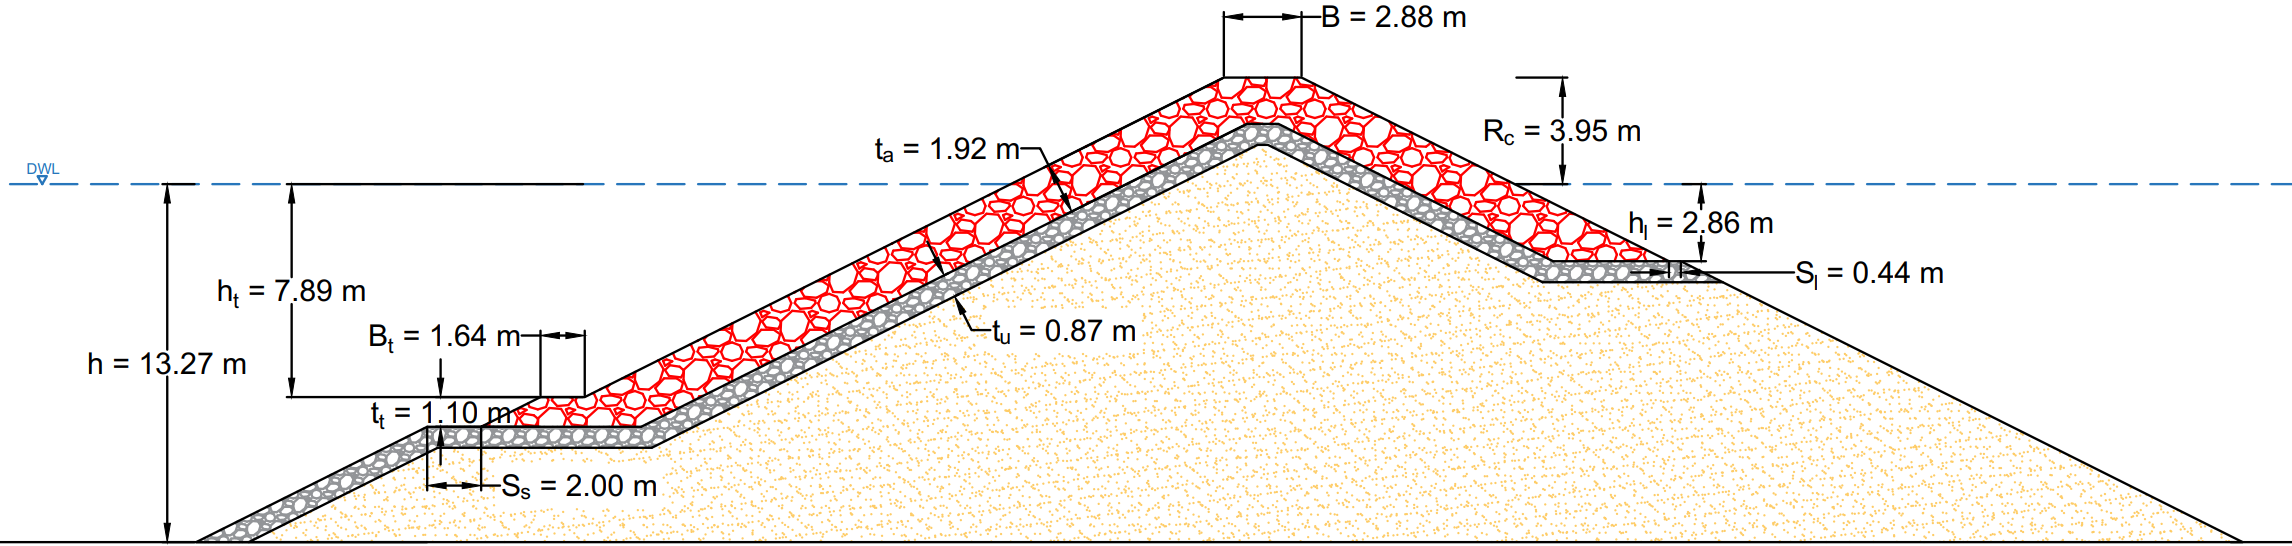
\includegraphics[width=0.95\textwidth]{Rubble_B.png}
    \caption{Selected natural rock rubble mound cross-section for Section B-B.}
    \label{fig:rubble_BB}
\end{figure}

\begin{figure}[H]
    \centering
    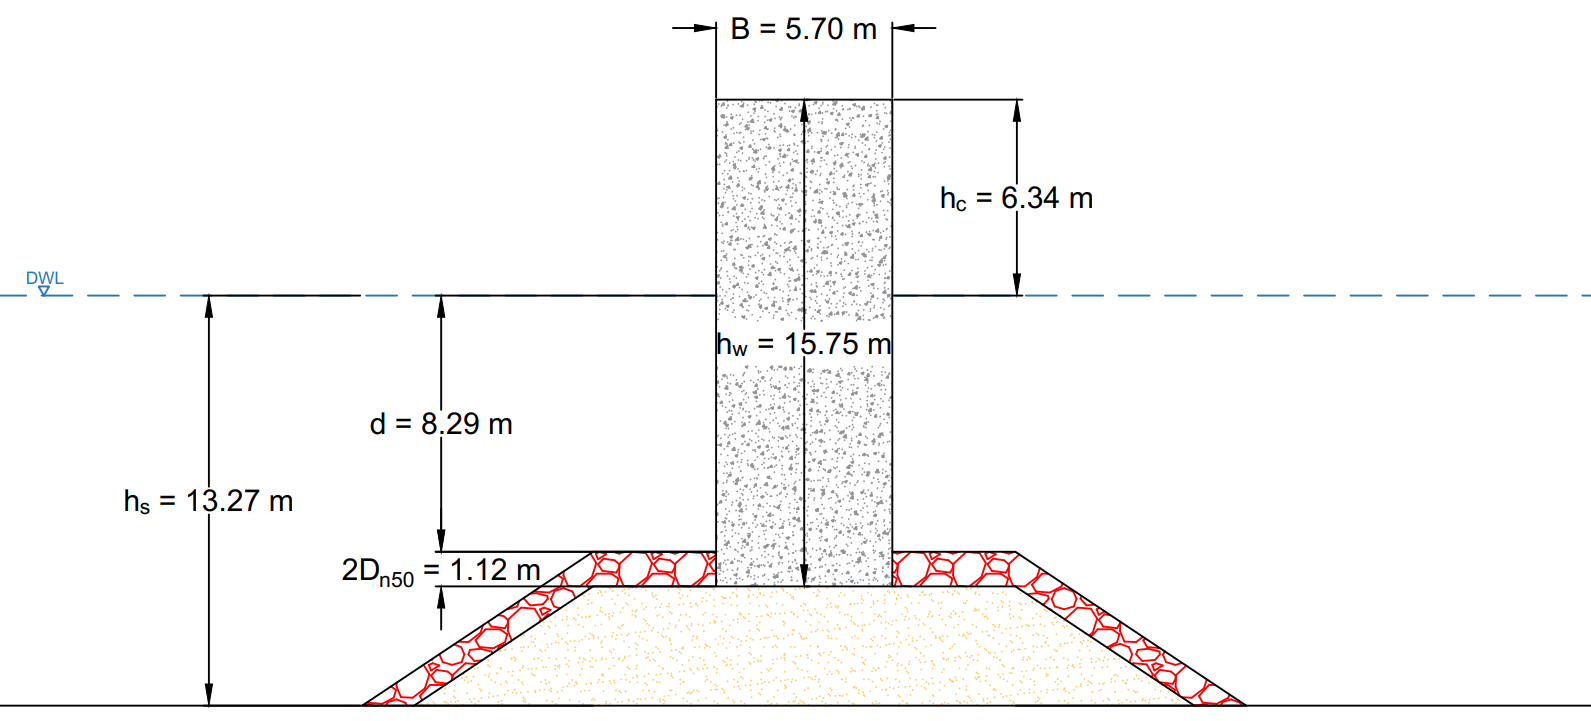
\includegraphics[width=0.90\textwidth]{Vert_B.png}
    \caption{Composite vertical wall alternative considered for Section B-B.}
    \label{fig:vertical_BB_alt}
\end{figure}


\subsubsection{Section C-C} \hspace*{0.5cm} Section C-C was designed as a floating breakwater, as required in the final exam statement. Therefore, unlike Sections A-A and B-B, no alternative structure type selection was carried out for this section. The purpose of the design was to check whether the selected floating body could satisfy the wave transmission, floating stability, force, and mooring requirements under the HWL condition. 

The wave height at the breakwater head was first reduced using the diffraction coefficient obtained from the SPM diffraction diagrams. With \(H_{head}=2.8040~\mathrm{m}\) and \(K_d=0.0724\), the incident wave height at Section C-C became \(H_i=0.2030~\mathrm{m}\). This value was already smaller than the allowable harbour agitation limit of \(H_{t,allow}=0.30~\mathrm{m}\). Therefore, the floating breakwater dimensions were not governed primarily by wave attenuation. 

The selected geometry was instead controlled by floating stability, especially the metacentric height required under eccentric loading. A freeboard of \(h_f=0.80~\mathrm{m}\) was adopted, and the ratio \(B_{fb}/h_d=3.0\) was used. This gave a draft of \(h_d=2.90~\mathrm{m}\), a floating breakwater width of \(B_{fb}=8.70~\mathrm{m}\), and a total height of \(3.70~\mathrm{m}\). The required wall thickness from buoyancy equilibrium was \(t=0.4801~\mathrm{m}\). 

The final geometry satisfied the transmission checks. The Wiegel and Macagno equations both gave transmitted wave heights below \(0.30~\mathrm{m}\), confirming that the section provides sufficient wave protection at C-C. The calculated metacentric height was \(GM=1.7750~\mathrm{m}\), which was slightly larger than the eccentric-loading requirement of \(1.7422~\mathrm{m}\). The resulting tilt angle was \(\Phi=0.10306~\mathrm{rad}\), which remained below the allowable value of \(0.105~\mathrm{rad}\). 

The total horizontal force used for the mooring design was \(P=28.8921~\mathrm{kN/m}\). The final mooring layout gave a projected length of \(11.5547~\mathrm{m}\), a chain length of \(11.8133~\mathrm{m}\), and a maximum line tension of \(30.2066~\mathrm{kN/m}\). These values were used to define the mooring layout shown in Figure~\ref{fig:float_C_side}. 

Overall, the selected floating breakwater satisfies the required functional and stability checks for Section C-C. The final section is governed more by floating stability and mooring requirements than by wave transmission, because the diffracted incident wave height is already below the allowable harbour agitation limit. 

\begin{figure}[H] 
    \centering 
    
\includegraphics[width=0.95\textwidth]{figures/Float_C.png} 
    \caption{Selected floating breakwater cross-section for Section C-C.} 
    \label{fig:float_C_section} 
\end{figure} 

\begin{figure}[H] 
    \centering 
    
\includegraphics[width=0.95\textwidth]{figures/Float_C_side.png} 
    \caption{Mooring layout for the selected floating breakwater at Section C-C.} 
    \label{fig:float_C_side} 
\end{figure}


% -------------------- Conclusion --------------------
\section{Conclusion}

\hspace*{0.5cm} In this study, preliminary breakwater designs were completed for the Ören/Milas Marina final project. The design covered Sections A-A, B-B, and C-C under the HWL condition. The offshore wave conditions given in the final exam statement were transformed to the design sections using SWANOne, and the resulting local wave parameters were used in the stability and dimensional calculations.

For Sections A-A and B-B, different breakwater alternatives were checked before selecting the final structure types. These alternatives included a conventional natural rock rubble mound, an X-Bloc armour, an Icelandic-type berm breakwater, and a composite vertical wall. The comparison was based not only on stability results, but also on constructability, footprint, crest elevation, material type, and suitability for marina conditions.

For Section A-A, the final selected structure was a natural rock rubble mound breakwater. Since the section is relatively shallow, the condition \(h/H_{s,toe}<3\) was satisfied and Van Gent (2003) was used for the final armour sizing. This resulted in an armour weight of \(3.5436~\mathrm{t}\) and \(D_{n50}=1.0949~\mathrm{m}\). The berm alternative required the same primary armour size after the shallow-water correction, so its advantage over the rubble mound became limited. The X-Bloc alternative required special concrete armour units and a higher crest elevation, while the vertical wall required a tall concrete structure and would be more reflective. Therefore, the natural rubble mound was considered the most suitable and balanced option for A-A.

For Section B-B, the natural rock rubble mound was also selected as the preferred final structure. The selected armour weight was \(2.3815~\mathrm{t}\), with \(D_{n50}=0.9590~\mathrm{m}\), based on Van der Meer (2021). The berm breakwater was technically feasible, but its benefit compared with the rubble mound was not large enough to justify the additional complexity. The X-Bloc option became less attractive because the row check required a \(5.0~\mathrm{m^3}\), \(12.0~\mathrm{t}\) unit. The composite vertical wall was a strong compact alternative for B-B, since it significantly reduced the required section width and satisfied the sliding and overturning checks. However, it also required a large concrete wall, more demanding marine construction, and would produce more wave reflection. For this reason, the rubble mound was kept as the selected design, while the vertical wall was presented as a feasible alternative if space becomes the main constraint.

For Section C-C, a floating breakwater was designed as required in the final exam statement. The incident wave height at C-C was obtained by applying the diffraction coefficient \(K_d=0.0724\) to the wave height near the breakwater head. The resulting wave height was \(H_i=0.2030~\mathrm{m}\), which was already below the allowable harbour agitation limit of \(0.30~\mathrm{m}\). Therefore, the floating breakwater dimensions were governed mainly by floating stability rather than wave transmission. The final design had a width of \(8.70~\mathrm{m}\), a draft of \(2.90~\mathrm{m}\), a freeboard of \(0.80~\mathrm{m}\), and a wall thickness of \(0.4801~\mathrm{m}\). The floating body satisfied the metacentric height, eccentric loading, force, and mooring checks. The floating breakwater alternative was also checked for Sections A-A and B-B, but it was not found suitable for these exposed locations. The incident wave heights were approximately \(3~\mathrm{m}\), and the wave period was about \(7.2~\mathrm{s}\), which are outside the usual practical range for floating breakwaters.


Overall, the selected design consists of natural rock rubble mound breakwaters for Sections A-A and B-B, and a floating breakwater for Section C-C. This combination provides a practical solution for the marina because the rubble mound sections are cost effective, dissipative, and easy to construct, while the floating breakwater satisfies the required functional conditions at C-C.


\newpage

% -------------------- References --------------------

\begin{thebibliography}{99}
\addcontentsline{toc}{section}{References}

\bibitem{RockManual}
CIRIA, CUR, CETMEF. (2007). \textit{The Rock Manual: The use of rock in hydraulic engineering} (2nd ed.). CIRIA.

\bibitem{DMC2023}
DMC. (2023). \textit{Xbloc \& XblocPlus design guidelines 2023}. Delta Marine Consultants.

\bibitem{ERA5}
European Centre for Medium-Range Weather Forecasts. (n.d.). \textit{ERA5 reanalysis}. https://www.ecmwf.int/

\bibitem{Ergin2019}
Ergin, A. (2019). \textit{Coastal engineering}. Middle East Technical University.

\bibitem{Guler2014}
Guler, H. G., Ergin, A., \& Ozyurt, G. (2014). A comparative study on the stability formulas of rubble mound breakwaters. \textit{Proceedings of the International Conference on Coastal Engineering 2014}.

\bibitem{JONSWAP1973}
Hasselmann, K., Barnett, T. P., Bouws, E., Carlson, H., Cartwright, D. E., Enke, K., Ewing, J. A., Gienapp, H., Hasselmann, D. E., Kruseman, P., Meerburg, A., M\"uller, P., Olbers, D. J., Richter, K., Sell, W., \& Walden, H. (1973). \textit{Measurements of wind-wave growth and swell decay during the Joint North Sea Wave Project (JONSWAP)}.

\bibitem{CE593}
Middle East Technical University, Department of Civil Engineering. (2025). \textit{CE 593 lecture notes} [Course notes].

\bibitem{CE598}
Middle East Technical University, Department of Civil Engineering. (2025). \textit{CE 598 lecture notes} [Course notes].

\bibitem{SPM1984}
U.S. Army Corps of Engineers. (1984). \textit{Shore protection manual}.

\bibitem{VdM1988}
Van der Meer, J. W. (1988). \textit{Rock slopes and gravel beaches under wave attack}. Delft Hydraulics.

\bibitem{VdM2021}
Van der Meer, J. W. (2021). Updated rock stability formulae with spectral period. \textit{Journal of Coastal and Hydraulic Structures, 1}.

\bibitem{EurOtop2018}
Van der Meer, J. W., Allsop, N. W. H., Bruce, T., De Rouck, J., Kortenhaus, A., Pullen, T., Sch\"{u}ttrumpf, H., Troch, P., \& Zanuttigh, B. (2018). \textit{EurOtop: Manual on wave overtopping of sea defences and related structures} (2nd ed.). www.overtopping-manual.com.

\bibitem{VdM1995}
Van der Meer, J. W., d'Angremond, K., \& Gerding, E. (1995). Toe structure stability of rubble mound breakwaters. In \textit{Proceedings of Advances in Coastal Structures and Breakwaters} (pp. 308--321). Thomas Telford.

\bibitem{VdMS2016chapter}
Van der Meer, J. W., \& Sigurdarson, S. (2016). Design of berm breakwaters. In Y. C. Kim (Ed.), \textit{Design of coastal structures and sea defenses}. World Scientific.

\bibitem{VdMS2016book}
Van der Meer, J. W., \& Sigurdarson, S. (2016). \textit{Design and construction of berm breakwaters}. World Scientific.

\bibitem{VanGent2003}
Van Gent, M. R. A., Smale, A. J., \& Kuiper, C. (2003). Stability of rock slopes with shallow foreshores. In J. A. Melby (Ed.), \textit{Coastal Structures 2003: Proceedings of the Conference} (pp. 100--112). American Society of Civil Engineers. https://doi.org/10.1061/40733(147)9

\bibitem{VanGent2007}
Van Gent, M. R. A., Van den Boogaard, H. F. P., Pozueta, B., \& Medina, J. R. (2007). Neural network modelling of wave overtopping at coastal structures. \textit{Coastal Engineering, 54}(8), 586--593.

\bibitem{WesselSmith1996}
Wessel, P., \& Smith, W. H. F. (1996). A global self-consistent, hierarchical, high-resolution shoreline database. \textit{Journal of Geophysical Research: Solid Earth, 101}(B4), 8741--8743.

\end{thebibliography}
\newpage

% -------------------- Appendix --------------------
\appendix
\section{Appendix}

\subsection{Rubble Mound Design Code}
\begin{lstlisting}[frame=single, numbers=left, style=Matlab-Pyglike]
% =========================================================
%  RUBBLE MOUND / X-BLOC BREAKWATER DESIGN
% =========================================================

clear; clc;

%% =========================================================
%  USER SECTION SELECTION
% =========================================================

section = 'A';

%% =========================================================
%  CONSTANTS
% =========================================================

g       = 9.81;
rho_air = 1.21;      % kg/m3
rho_w   = 1020;      % kg/m3

%% =========================================================
%  PROJECT OFFSHORE DESIGN WAVE
% =========================================================

Hs0 = 3.07;              % m, offshore significant wave height
Ts0 = 6.58;              % s, offshore significant wave period
Tp0 = 1.1 * Ts0;         % s, converted offshore peak period
L0  = 1.56 * Tp0^2;      % m, deep-water wavelength
s0  = Hs0 / L0;          % deep-water wave steepness

%% =========================================================
%  SECTION-SPECIFIC INPUTS
% =========================================================

switch section

    case 'B'

        is_head = false;

        h_NWL = 12.0000;

        Hm0_toe = 2.81482;        % m, Hm0/Hsig from SWANOne
        Tp      = 7.2016;         % s, RTpeak
        Tm01    = 6.0143;         % s, Tm01
        Tm10    = 6.5193;         % s, Tm-1,0
        H13     = 2.8687753;      % m, H1/3
        H2pct   = 4.0073712;      % m, H2%
        H1_10   = 3.6467483;      % m, H1/10

        Hs_toe  = H13;            % m, design wave height used in armor equations

        swan_depth = 12.0631;

    case 'A'

        is_head = false;

        h_NWL = 5.5;

        Hm0_toe = 2.83387;        % m, Hm0/Hsig from SWANOne
        Tp      = 7.2016;         % s, RTpeak
        Tm01    = 5.8769;         % s, Tm01
        Tm10    = 6.4599;         % s, Tm-1,0
        H13     = 3.1108699;      % m, H1/3
        H2pct   = 4.3455514;      % m, H2%
        H1_10   = 3.9544957;      % m, H1/10

        Hs_toe  = H13;            % m, design wave height used in armor equations

        swan_depth = 5.5853;

    otherwise

        error('Unknown section. Use section = ''B-B'' or section = ''A-A''.');

end

%% =========================================================
%  MATERIAL PARAMETERS
% =========================================================

gs = 2.700;              % t/m3, quarrystone density
gw = 1.025;              % t/m3, seawater density

Delta = gs/gw - 1;
Sr    = gs/gw;

%% =========================================================
%  SLOPE AND HYDRAULIC REDUCTION PARAMETERS
% =========================================================

cot_a = 2;             % 1V:2H
tana  = 1 / cot_a;

a0       = 0;            % wave attack angle [deg]
gam_b    = 1.0;
gam_f    = 0.40;         % roughness factor for natural rock
gam_beta = 1 - 0.0063*a0;

gam_f_xbloc = 0.44;      % roughness factor for XBloc

%% =========================================================
%  HUDSON PARAMETERS
% =========================================================

KD_nb_trunk = 4.0;
KD_b_trunk  = 2.0;

KD_nb_head  = 2.8;
KD_b_head   = 1.6;

%% =========================================================
%  VAN DER MEER PARAMETERS
% =========================================================

P_vdm = 0.4;
S     = 2;
N     = 3000;

%% =========================================================
%  CROSS-SECTION PARAMETERS
% =========================================================

n_armor     = 2;
k_delta     = 1.00;
ratio_ul    = 2.2;
n_crest     = 3;
head_factor = 1.5;

%% =========================================================
%  X-BLOC PARAMETERS
% =========================================================

rho_c_x = 2.400;         % t/m3
rho_w_x = 1.030;         % t/m3
Delta_x = (rho_c_x - rho_w_x) / rho_w_x;

%% =========================================================
%  DESIGN WATER LEVEL
% =========================================================

DWL_HWL = 1.2697;      % m HWL
DWL = DWL_HWL;

h = h_NWL + DWL_HWL;

%% =========================================================
%  INPUT SUMMARY
% =========================================================

fprintf('\n======================================================\n');
fprintf('DESIGN INPUT SUMMARY: SECTION %s, HWL ONLY\n', section);
fprintf('======================================================\n');

fprintf('Section treated as head?   = %s\n', yesno(is_head));
fprintf('Hs0 offshore              = %.4f m\n', Hs0);
fprintf('Ts0 offshore              = %.4f s\n', Ts0);
fprintf('Tp0 offshore              = %.4f s\n', Tp0);
fprintf('L0                        = %.4f m\n', L0);
fprintf('s0                        = %.4f\n', s0);
fprintf('SWAN Hm0,toe              = %.4f m\n', Hm0_toe);
fprintf('Hs,toe used in equations  = %.4f m\n', Hs_toe);
fprintf('SWAN Tp                   = %.4f s\n', Tp);
fprintf('SWAN Tm01                 = %.4f s\n', Tm01);
fprintf('SWAN Tm-1,0               = %.4f s\n', Tm10);
fprintf('SWAN H1/3                 = %.4f m\n', H13);
fprintf('SWAN H2%%                  = %.4f m\n', H2pct);
fprintf('SWAN H1/10                = %.4f m\n', H1_10);
fprintf('h used in design          = %.4f m\n', h);
fprintf('cot_a                     = %.4f\n', cot_a);
fprintf('NOTE: Hs,toe is set equal to H1/3 for armor sizing, not Hm0.\n');


%% =========================================================
%  RUN-UP
% =========================================================

fprintf('\n======================================================\n');
fprintf('RUN-UP: SECTION %s, HWL\n', section);
fprintf('======================================================\n');

xi_m10 = tana / sqrt(2*pi*Hs_toe / (g*Tm10^2));

Ru_1 = 1.75 * gam_b * gam_f * gam_beta * xi_m10 * Hs_toe;

gam_f_surg = gam_f + (xi_m10 - 1.8) * (1 - gam_f) / 8.2;
gam_f_surg = min(max(gam_f_surg, gam_f), 1.0);

Ru_2 = 1.07 * gam_f_surg * gam_beta * ...
    (4.0 - 1.5 / sqrt(gam_b * xi_m10)) * Hs_toe;

Ru_2pct = min(Ru_1, Ru_2);

fprintf('xi_m-1,0                 = %.4f\n', xi_m10);
fprintf('Ru,2%% Eq. 5.1             = %.4f m\n', Ru_1);
fprintf('Ru,2%% Eq. 5.2             = %.4f m\n', Ru_2);
fprintf('Governing Ru,2%%          = %.4f m\n', Ru_2pct);

%% =========================================================
%  CREST HEIGHT BY OVERTOPPING
% =========================================================

fprintf('\n======================================================\n');
fprintf('CREST HEIGHT: SECTION %s, HWL\n', section);
fprintf('======================================================\n');

q_design = 1e-3;     % m3/s/m = 1 L/s/m

inner = q_design / (0.1035 * sqrt(g * Hs_toe^3));

if inner <= 0 || inner >= 1
    warning('Overtopping equation inner term is outside the expected range.');
end

Rc_rock = Hs_toe * gam_f * gam_beta / 1.35 * (-log(inner))^(1/1.3);
crest_rock = DWL + Rc_rock;

Rc_xbloc = Hs_toe * gam_f_xbloc * gam_beta / 1.35 * (-log(inner))^(1/1.3);
crest_xbloc = DWL + Rc_xbloc;
RFB_xbloc = Rc_xbloc / Hs_toe;

fprintf('q_design                  = %.6f m3/s/m\n', q_design);
fprintf('Rock Rc                   = %.4f m\n', Rc_rock);
fprintf('Rock crest elevation      = %.4f m MSL\n', crest_rock);
fprintf('XBloc Rc                  = %.4f m\n', Rc_xbloc);
fprintf('XBloc crest elevation     = %.4f m MSL\n', crest_xbloc);
fprintf('XBloc RFB                 = %.4f\n', RFB_xbloc);

%% =========================================================
%  HUDSON
% =========================================================

fprintf('\n======================================================\n');
fprintf('HUDSON: SECTION %s, HWL\n', section);
fprintf('======================================================\n');

Hs_hudson = H1_10;
ratio_H_h = Hs_hudson / h;

if is_head
    if ratio_H_h < 0.6
        KD = KD_nb_head;
        tag_break = 'non-breaking';
    else
        KD = KD_b_head;
        tag_break = 'breaking';
    end
else
    if ratio_H_h < 0.6
        KD = KD_nb_trunk;
        tag_break = 'non-breaking';
    else
        KD = KD_b_trunk;
        tag_break = 'breaking';
    end
end

W_Hudson = gs * Hs_hudson^3 * tana / ((Sr - 1)^3 * KD);

fprintf('H1/10                     = %.4f m\n', Hs_hudson);
fprintf('H1/10 / h                 = %.4f\n', ratio_H_h);
fprintf('Breaking condition        = %s\n', tag_break);
fprintf('KD                        = %.4f\n', KD);
fprintf('Hudson W                  = %.4f t\n', W_Hudson);

%% =========================================================
%  VAN DER MEER 1988
% =========================================================

fprintf('\n======================================================\n');
fprintf('VAN DER MEER 1988: SECTION %s, HWL\n', section);
fprintf('======================================================\n');

Tm_vdm88 = 0.81 * (Tp / 1.08);

xi_m = tana / sqrt(2*pi*Hs_toe / (g*Tm_vdm88^2));
xi_cr_88 = (6.2 * P_vdm^0.31 * sqrt(tana))^(1/(P_vdm+0.5));

if xi_m < xi_cr_88
    RHS_88 = 6.2 * P_vdm^0.18 * (S/sqrt(N))^0.2 * xi_m^(-0.5);
    type_88 = 'Plunging';
else
    RHS_88 = 1.0 * P_vdm^(-0.13) * (S/sqrt(N))^0.2 * sqrt(cot_a) * xi_m^P_vdm;
    type_88 = 'Surging';
end

Dn50_VdM88 = Hs_toe / (Delta * RHS_88);
W_VdM88 = gs * Dn50_VdM88^3;

fprintf('Tm                        = %.4f s\n', Tm_vdm88);
fprintf('xi_m                      = %.4f\n', xi_m);
fprintf('xi_cr                     = %.4f\n', xi_cr_88);
fprintf('Breaker type              = %s\n', type_88);
fprintf('Dn50 VdM88                = %.4f m\n', Dn50_VdM88);
fprintf('W VdM88                   = %.4f t\n', W_VdM88);

%% =========================================================
%  VAN DER MEER 2021
% =========================================================

fprintf('\n======================================================\n');
fprintf('VAN DER MEER 2021: SECTION %s, HWL\n', section);
fprintf('======================================================\n');

xi_m10 = tana / sqrt(2*pi*Hs_toe / (g*Tm10^2));
xi_cr_21 = (6.49/0.97 * P_vdm^0.31 * sqrt(tana))^(1/(P_vdm+0.5));

if xi_m10 < xi_cr_21
    RHS_21 = 6.49 * P_vdm^0.18 * (S/sqrt(N))^0.2 * xi_m10^(-0.5);
    type_21 = 'Plunging';
else
    RHS_21 = 0.97 * P_vdm^(-0.13) * (S/sqrt(N))^0.2 * sqrt(cot_a) * xi_m10^P_vdm;
    type_21 = 'Surging';
end

Dn50_VdM21 = Hs_toe / (Delta * RHS_21);
W_VdM21 = gs * Dn50_VdM21^3;

fprintf('Tm-1,0                    = %.4f s\n', Tm10);
fprintf('xi_m-1,0                  = %.4f\n', xi_m10);
fprintf('xi_cr                     = %.4f\n', xi_cr_21);
fprintf('Breaker type              = %s\n', type_21);
fprintf('Dn50 VdM21                = %.4f m\n', Dn50_VdM21);
fprintf('W VdM21                   = %.4f t\n', W_VdM21);

fprintf('\nVdM comparison:\n');
fprintf('VdM88 W                   = %.4f t\n', W_VdM88);
fprintf('VdM21 W                   = %.4f t\n', W_VdM21);
fprintf('Difference                = %+.2f %%\n', (W_VdM21 - W_VdM88)/W_VdM88*100);

%% =========================================================
%  VAN GENT 2004
% =========================================================

fprintf('\n======================================================\n');
fprintf('VAN GENT 2003: SECTION %s, HWL\n', section);
fprintf('======================================================\n');

xi_cr_VG = (8.4/1.3 * P_vdm^0.31 * sqrt(tana))^(1/(P_vdm+0.5));

if xi_m10 < xi_cr_VG
    RHS_VG = 8.4 * P_vdm^0.18 * (S/sqrt(N))^0.2 * ...
        (Hs_toe/H2pct) * xi_m10^(-0.5);
    type_VG = 'Plunging';
else
    RHS_VG = 1.3 * P_vdm^(-0.13) * (S/sqrt(N))^0.2 * ...
        (Hs_toe/H2pct) * sqrt(cot_a) * xi_m10^P_vdm;
    type_VG = 'Surging';
end

Dn50_VG = Hs_toe / (Delta * RHS_VG);
W_VG = gs * Dn50_VG^3;

fprintf('H2%%                       = %.4f m\n', H2pct);
fprintf('xi_m-1,0                  = %.4f\n', xi_m10);
fprintf('xi_cr                     = %.4f\n', xi_cr_VG);
fprintf('Breaker type              = %s\n', type_VG);
fprintf('Dn50 Van Gent             = %.4f m\n', Dn50_VG);
fprintf('W Van Gent                = %.4f t\n', W_VG);

%% =========================================================
%  DESIGN METHOD SELECTION
%% =========================================================

fprintf('\n======================================================\n');
fprintf('DESIGN METHOD SELECTION: SECTION %s, HWL\n', section);
fprintf('======================================================\n');

C1 = h / Hs_toe;
C2 = H2pct / Hs_toe;
C3 = Hs_toe / Hs0;

fprintf('C1: h/Hs,toe              = %.4f < 3   ? %s\n', C1, yesno(C1 < 3));
fprintf('C2: H2%%/Hs,toe            = %.4f < 1.4 ? %s\n', C2, yesno(C2 < 1.4));
fprintf('C3: Hs,toe/Hs0            = %.4f < 0.9 ? %s\n', C3, yesno(C3 < 0.9));

if C1 < 3
    W_base = W_VG;
    Dn50_base = Dn50_VG;
    method = 'Van Gent 2004';
    method_reason = 'selected because h/Hs,toe < 3';
else
    W_base = W_VdM21;
    Dn50_base = Dn50_VdM21;
    method = 'Van der Meer 2021';
    method_reason = 'selected because h/Hs,toe >= 3';
end

if is_head
    W_design = W_base * head_factor;
    method_note = sprintf('%s with head factor %.1f', method, head_factor);
else
    W_design = W_base;
    method_note = method;
end

Dn50_design = (W_design / gs)^(1/3);

fprintf('Selected method            = %s\n', method_note);
fprintf('Reason                     = %s\n', method_reason);
fprintf('W_design                   = %.4f t\n', W_design);
fprintf('Dn50_design                = %.4f m\n', Dn50_design);

%% =========================================================
%  NATURAL ROCK CROSS-SECTION
% =========================================================

fprintf('\n======================================================\n');
fprintf('NATURAL ROCK CROSS-SECTION: SECTION %s, HWL\n', section);
fprintf('======================================================\n');

Dn50_r = Dn50_design;
W_r    = W_design;

t_arm = n_armor * k_delta * Dn50_r;

Dn50_ul = Dn50_r / ratio_ul;
W_ul    = gs * Dn50_ul^3;
t_ul    = n_armor * k_delta * Dn50_ul;

B_crest = n_crest * k_delta * Dn50_r;

W_core_min = W_design / 4000;
W_core_max = W_design / 200;

% ---- Rock toe design ------------------------------------
Nod_toe = 0.5;
ht_toe_ratio = 0.6;

ht_toe = ht_toe_ratio * h;

Dn50_toe_calc = Hs_toe / ((2 + 6.2*(ht_toe/h)^2.7) * Nod_toe^0.15 * Delta);

Dn50_toe_rock = max(Dn50_toe_calc, Dn50_ul);
W_toe_rock    = gs * Dn50_toe_rock^3;

toe_thk_rock = 2 * Dn50_toe_rock;
toe_len_rock = 3 * Dn50_toe_rock;
toe_elev     = DWL - ht_toe;

fprintf('W_design                  = %.4f t\n', W_design);
fprintf('Dn50 armor                = %.4f m\n', Dn50_r);
fprintf('Armor layer thickness     = %.4f m\n', t_arm);
fprintf('Underlayer Dn50           = %.4f m\n', Dn50_ul);
fprintf('Underlayer W              = %.4f t\n', W_ul);
fprintf('Underlayer thickness      = %.4f m\n', t_ul);
fprintf('Crest width B             = %.4f m\n', B_crest);
fprintf('Core W range              = %.6f - %.6f t\n', W_core_min, W_core_max);
fprintf('Toe ht                    = %.4f m\n', ht_toe);
fprintf('Toe elevation             = %.4f m MSL\n', toe_elev);
fprintf('Rock toe Dn50 calculated  = %.4f m\n', Dn50_toe_calc);
fprintf('Rock toe Dn50 selected    = %.4f m\n', Dn50_toe_rock);
fprintf('Rock toe W selected       = %.4f t\n', W_toe_rock);
fprintf('Rock toe thickness        = %.4f m\n', toe_thk_rock);
fprintf('Rock toe length           = %.4f m\n', toe_len_rock);
fprintf('Rock crest elevation      = %.4f m MSL\n', crest_rock);

%% =========================================================
%  X-BLOC DESIGN
% =========================================================

fprintf('\n======================================================\n');
fprintf('X-BLOC DESIGN: SECTION %s, HWL\n', section);
fprintf('======================================================\n');

fprintf('Delta_x                   = %.4f\n', Delta_x);

V_table  = [0.75,1,1.5,2,2.5,3,4,5,6,7,8,9,10,12,14,16,18,20];
D_table  = [1.31,1.44,1.65,1.82,1.96,2.08,2.29,2.47,2.62,2.76,...
            2.88,3.00,3.11,3.30,3.48,3.63,3.78,3.91];
Dy_table = [0.83,0.91,1.04,1.14,1.23,1.31,1.44,1.55,1.65,1.74,...
            1.82,1.89,1.96,2.08,2.19,2.29,2.38,2.47];

CF_depth = 2.0;

V_base = (Hm0_toe / (2.77 * Delta_x))^3;
V_CF   = V_base * CF_depth;

idxV = find(V_table >= V_CF, 1, 'first');

if isempty(idxV)
    V_design_x = V_table(end);
    warning('Required XBloc volume exceeds table maximum. Largest table value used.');
else
    V_design_x = V_table(idxV);
end

fprintf('V_base                    = %.4f m3\n', V_base);
fprintf('CF_depth                  = %.4f\n', CF_depth);
fprintf('V_CF                      = %.4f m3\n', V_CF);
fprintf('Initial V_design          = %.4f m3\n', V_design_x);

idx_initial = find(V_table == V_design_x, 1, 'first');
D_initial  = D_table(idx_initial);
Dy_initial = Dy_table(idx_initial);

L_slope = h * sqrt(1 + cot_a^2);
nrows_initial = (L_slope - 0.5 * D_initial) / Dy_initial;

fprintf('\n--- Row check ---\n');
fprintf('Vertical height h         = %.4f m\n', h);
fprintf('Slope length              = %.4f m\n', L_slope);
fprintf('Rows with initial V       = %.4f\n', nrows_initial);
fprintf('Rows <= 20 ?              = %s\n', yesno(nrows_initial <= 20));

V_final_x = V_design_x;

for jj = 1:length(V_table)
    if 19 * Dy_table(jj) + 0.5 * D_table(jj) >= L_slope
        V_final_x = max(V_design_x, V_table(jj));
        break;
    end
end

idx_final = find(V_table == V_final_x, 1, 'first');

D_xbloc  = D_table(idx_final);
Dy_xbloc = Dy_table(idx_final);

nrows_final = (L_slope - 0.5 * D_xbloc) / Dy_xbloc;

fprintf('\n--- Final XBloc size ---\n');
fprintf('V_final                   = %.4f m3\n', V_final_x);
fprintf('D                         = %.4f m\n', D_xbloc);
fprintf('Dy                        = %.4f m\n', Dy_xbloc);
fprintf('Rows with final V         = %.4f\n', nrows_final);

% ---- X-BLOC UNDERLAYER ----------------------------------

W_unit_x = V_final_x * rho_c_x;

W_ul_min_x = W_unit_x / 15;
W_ul_max_x = W_unit_x / 6;

W_ul_sel_x = W_ul_min_x + 0.75 * (W_ul_max_x - W_ul_min_x);

Dn50_ul_x = (W_ul_sel_x / gs)^(1/3);
t_ul_x    = 2 * Dn50_ul_x;

fprintf('\n--- XBloc underlayer ---\n');
fprintf('XBloc unit weight         = %.4f t\n', W_unit_x);
fprintf('Underlayer W50 range      = %.4f - %.4f t\n', W_ul_min_x, W_ul_max_x);
fprintf('Selected W50              = %.4f t\n', W_ul_sel_x);
fprintf('Selected Dn50             = %.4f m\n', Dn50_ul_x);
fprintf('Underlayer thickness      = %.4f m\n', t_ul_x);

%% =========================================================
%  X-BLOC TOE DESIGN
% =========================================================

fprintf('\n======================================================\n');
fprintf('X-BLOC TOE DESIGN: SECTION %s, HWL\n', section);
fprintf('======================================================\n');

Nod_toe_x = 0.5;
Delta_r   = gs/gw - 1;

filter_thickness = 0.6;

W_found     = W_unit_x / 30;
Dn50_found  = (W_found / gs)^(1/3);

found_length    = Hs_toe;
found_thickness = Dn50_found;

Dn50_toe_x = max(Dn50_ul_x, 0.5);

for iter = 1:200

    toe_thk_x = 2 * Dn50_toe_x;
    ht_x = h - (filter_thickness + found_thickness + toe_thk_x);

    if ht_x <= 0
        ht_x = 0.1;
    end

    Dn50_new_x = Hs_toe / ((2 + 6.2*(ht_x/h)^2.7) * Nod_toe_x^0.15 * Delta_r);

    Dn50_new_x = max(Dn50_new_x, Dn50_ul_x);

    if abs(Dn50_new_x - Dn50_toe_x) < 1e-9
        break;
    end

    Dn50_toe_x = Dn50_new_x;

end

toe_thickness_x = 2 * Dn50_toe_x;
toe_length_x    = 3 * Dn50_toe_x;

ht_final_x = h - (filter_thickness + found_thickness + toe_thickness_x);

if ht_final_x <= 0
    ht_final_x = 0.1;
end

W_toe_x = gs * Dn50_toe_x^3;

fprintf('Granular filter thickness = %.4f m\n', filter_thickness);
fprintf('Foundation W              = %.4f t\n', W_found);
fprintf('Foundation Dn50           = %.4f m\n', Dn50_found);
fprintf('Foundation length         = %.4f m\n', found_length);
fprintf('Foundation thickness      = %.4f m\n', found_thickness);
fprintf('ht                        = %.4f m\n', ht_final_x);
fprintf('Rock toe Dn50             = %.4f m\n', Dn50_toe_x);
fprintf('Rock toe W                = %.4f t\n', W_toe_x);
fprintf('Rock toe thickness        = %.4f m\n', toe_thickness_x);
fprintf('Rock toe length           = %.4f m\n', toe_length_x);

%% =========================================================
%  FINAL DESIGN SUMMARY
% =========================================================

fprintf('\n\n======================================================\n');
fprintf('FINAL DESIGN SUMMARY: SECTION %s, HWL ONLY\n', section);
fprintf('======================================================\n');

fprintf('\n--- Hydraulic design basis ---\n');
fprintf('DWL_HWL                   = %.4f m MSL\n', DWL_HWL);
fprintf('Design depth h            = %.4f m\n', h);
fprintf('SWAN Hm0,toe              = %.4f m\n', Hm0_toe);
fprintf('Hs,toe used in equations  = %.4f m\n', Hs_toe);
fprintf('Tp                        = %.4f s\n', Tp);
fprintf('Tm-1,0                    = %.4f s\n', Tm10);
fprintf('H2%%                       = %.4f m\n', H2pct);
fprintf('H1/10                     = %.4f m\n', H1_10);
fprintf('Ru,2%%                     = %.4f m\n', Ru_2pct);

fprintf('\n--- Natural rock design ---\n');
fprintf('Selected method            = %s\n', method_note);
fprintf('Rock W_design              = %.4f t\n', W_design);
fprintf('Rock Dn50                  = %.4f m\n', Dn50_r);
fprintf('Armor layer thickness      = %.4f m\n', t_arm);
fprintf('Underlayer Dn50            = %.4f m\n', Dn50_ul);
fprintf('Underlayer W               = %.4f t\n', W_ul);
fprintf('Underlayer thickness       = %.4f m\n', t_ul);
fprintf('Crest width B              = %.4f m\n', B_crest);
fprintf('Crest elevation            = %.4f m MSL\n', crest_rock);
fprintf('Toe Dn50                   = %.4f m\n', Dn50_toe_rock);
fprintf('Toe W                      = %.4f t\n', W_toe_rock);
fprintf('Toe thickness              = %.4f m\n', toe_thk_rock);
fprintf('Toe length                 = %.4f m\n', toe_len_rock);
fprintf('Toe elevation              = %.4f m MSL\n', toe_elev);

fprintf('\n--- XBloc design ---\n');
fprintf('XBloc V_final              = %.4f m3\n', V_final_x);
fprintf('XBloc unit weight          = %.4f t\n', W_unit_x);
fprintf('XBloc D                    = %.4f m\n', D_xbloc);
fprintf('XBloc Dy                   = %.4f m\n', Dy_xbloc);
fprintf('XBloc rows                 = %.4f\n', nrows_final);
fprintf('XBloc Rc                   = %.4f m\n', Rc_xbloc);
fprintf('XBloc crest elevation      = %.4f m MSL\n', crest_xbloc);
fprintf('XBloc underlayer W50       = %.4f t\n', W_ul_sel_x);
fprintf('XBloc underlayer Dn50      = %.4f m\n', Dn50_ul_x);
fprintf('XBloc underlayer thickness = %.4f m\n', t_ul_x);
fprintf('XBloc toe Dn50             = %.4f m\n', Dn50_toe_x);
fprintf('XBloc toe W                = %.4f t\n', W_toe_x);
fprintf('XBloc toe thickness        = %.4f m\n', toe_thickness_x);
fprintf('XBloc toe length           = %.4f m\n', toe_length_x);

%% =========================================================
%  LOCAL FUNCTION
% =========================================================

function s = yesno(val)
    if val
        s = 'YES';
    else
        s = 'NO';
    end
end
\end{lstlisting}

\subsection{Berm Design Code}
\begin{lstlisting}[frame=single, numbers=left, style=Matlab-Pyglike]

% =========================================================
%  BERM BREAKWATER DESIGN
% =========================================================

clear; clc;

%% ---- CONSTANTS ------------------------------------------
g  = 9.81;
gs = 2.700;       % t/m3, quarrystone
gw = 1.025;       % t/m3, seawater

Delta = gs/gw - 1;

%% ---- DESIGN WATER LEVEL --------------------------
DWL_HWL   = 1.2697;      % m MSL, from HWL calculation
tide_high = 0.20;        % m MSL, MHWS/high tide component
Delta_w   = 1.0;         % m, construction safety margin

%% ---- ROCK CLASS SELECTION --------------------

HsD_assumed_for_table = 3.0;       % m

ClassI_name  = 'Class I: 1-4 t';
M50_I_input  = 2.5;               % t

ClassII_name = 'Class II: 0.2-1 t underlayer';
M50_II_input = sqrt(0.2*1.0);     % t

useClassIII  = false;
ClassIII_name = 'No separate Class III';
M50_III_input = NaN;

P_resil = 20;                     % %

%% ---- SECTION INPUTS -------------------------------------
sections(1).name      = 'B-B';
sections(1).h_NWL_ref = 12.0000;
sections(1).HsD       = 2.81482;
sections(1).Tp        = 7.2016;
sections(1).H13       = 2.8687753;
sections(1).H2pct     = 4.0073712;
sections(1).Tm01      = 6.0143;
sections(1).Tm10      = 6.5193;
sections(1).cot_ad    = 1.5;

sections(2).name      = 'A-A';
sections(2).h_NWL_ref = 5.5000;
sections(2).HsD       = 2.83387;
sections(2).Tp        = 7.2016;
sections(2).H13       = 3.1108699;
sections(2).H2pct     = 4.3455514;
sections(2).Tm01      = 5.8769;
sections(2).Tm10      = 6.4599;
sections(2).cot_ad    = 2.0;      % A-A changed to 1V:2H for Van Gent shallow-water validity

%% ---- RUN ALL SECTIONS -----------------------------------
results = repmat(empty_berm_result(), numel(sections), 1);

for isec = 1:numel(sections)

    results(isec) = run_berm_design( ...
        sections(isec).name, ...
        sections(isec).h_NWL_ref, ...
        sections(isec).HsD, ...
        sections(isec).Tp, ...
        sections(isec).H13, ...
        sections(isec).H2pct, ...
        sections(isec).Tm01, ...
        sections(isec).Tm10, ...
        sections(isec).cot_ad, ...
        DWL_HWL, tide_high, Delta_w, ...
        g, gs, gw, Delta, ...
        HsD_assumed_for_table, ...
        ClassI_name, M50_I_input, ...
        ClassII_name, M50_II_input, ...
        useClassIII, ClassIII_name, M50_III_input, ...
        P_resil);

end

%% ---- FINAL COMPARISON TABLE -----------------------------
T = struct2table(results);

fprintf('\n\n============================================================\n');
fprintf('BERM DECISION METRICS TABLE\n');
fprintf('============================================================\n');
disp(T(:, {'Section','Structure','cot_alpha','HsD','h_DWL','Primary_W_t','Primary_Dn50_m', ...
           'Crest_elev_mMSL','Crest_width_m','Berm_width_m','Ah_m','Toe_elev_mMSL', ...
           'Approx_front_width_m','Ns_design','Ns_overload','Classification','Main_note'}));

writetable(T, 'berm_decision_metrics.csv');
fprintf('Saved: berm_decision_metrics.csv\n');

%% =========================================================
%  LOCAL DESIGN FUNCTION
%% =========================================================

function R = run_berm_design(section, h_NWL_ref, HsD, Tp, H13, H2pct, Tm01, Tm10, cot_ad, DWL_HWL, tide_high, Delta_w, g, gs, gw, Delta, HsD_assumed_for_table, ClassI_name, M50_I_input, ClassII_name, M50_II_input, useClassIII, ClassIII_name, M50_III_input, P_resil)
h_DWL = h_NWL_ref + DWL_HWL;
HsOL  = 1.2 * HsD;

fprintf('\n\n============================================================\n');
fprintf('===== GOVERNING CONDITIONS: SECTION %s, HWL =====\n', section);
fprintf('============================================================\n');
fprintf('DWL_HWL       = %.4f m MSL\n', DWL_HWL);
fprintf('h_NWL         = %.4f m\n', h_NWL_ref);
fprintf('h at DWL      = %.4f m\n', h_DWL);
fprintf('HsD actual    = %.4f m\n', HsD);
fprintf('HsD table     = %.4f m\n', HsD_assumed_for_table);
fprintf('HsOL          = %.4f m\n', HsOL);
fprintf('Tp            = %.4f s\n', Tp);
fprintf('MHWS          = %.4f m MSL\n', tide_high);
fprintf('Delta_w       = %.4f m\n\n', Delta_w);

%% =========================================================
%  CLASS I ROCK SIZING
%% =========================================================

M50_I = M50_I_input;
Dn50_I = (M50_I/gs)^(1/3);
ClassI_source = 'lecture-table representative Class I rock';

if strcmp(section, 'A-A')
    fprintf('===== VAN GENT SHALLOW-WATER VALIDITY CHECK FOR CLASS I =====\n');

    Hs0_project = 3.0700;
    Hs_VG = H13;
    H2_VG = H2pct;
    Tm_VG = Tm01;
    Tm10_VG = Tm10;

    P_VG = 0.40;
    Sd_VG = 2;
    N_VG = 3000;

    c_pl = 8.4;
    c_s  = 1.3;

    tan_alpha_VG = 1/cot_ad;

    som_VG = 2*pi*Hs_VG/(g*Tm_VG^2);
    xi_m_VG = tan_alpha_VG/sqrt(2*pi*Hs_VG/(g*Tm_VG^2));
    xi_s_VG = tan_alpha_VG/sqrt(2*pi*Hs_VG/(g*Tm10_VG^2));

    H2_Hs_ratio = H2_VG/Hs_VG;
    Hs0_h_ratio = Hs0_project/h_DWL;

    xi_cr_VG = ((c_pl/c_s)*P_VG^0.31*sqrt(tan_alpha_VG))^(1/(P_VG+0.5));

    if xi_s_VG < xi_cr_VG
        RHS_VG = c_pl*P_VG^0.18*(Sd_VG/sqrt(N_VG))^0.2*(Hs_VG/H2_VG)*xi_s_VG^(-0.5);
        type_VG = 'Plunging';
    else
        RHS_VG = c_s*P_VG^(-0.13)*(Sd_VG/sqrt(N_VG))^0.2*(Hs_VG/H2_VG)*sqrt(cot_ad)*xi_s_VG^P_VG;
        type_VG = 'Surging';
    end

    Dn50_VG = Hs_VG/(Delta*RHS_VG);
    M50_VG = gs*Dn50_VG^3;
    Ns_VG = Hs_VG/(Delta*Dn50_VG);

    slope_ok = cot_ad >= 2.0 && cot_ad <= 4.0;
    N_ok     = N_VG <= 3000;
    som_ok   = som_VG >= 0.01 && som_VG <= 0.06;
    xi_m_ok  = xi_m_VG >= 1.0 && xi_m_VG <= 5.0;
    xi_s_ok  = xi_s_VG >= 1.3 && xi_s_VG <= 6.5;
    H2Hs_ok  = H2_Hs_ratio >= 1.2 && H2_Hs_ratio <= 1.4;
    Hs0h_ok  = Hs0_h_ratio >= 0.25 && Hs0_h_ratio <= 1.5;
    Ns_ok    = Ns_VG >= 0.5 && Ns_VG <= 4.5;
    Sd_ok    = Sd_VG < 30;

    vg_valid = slope_ok && N_ok && som_ok && xi_m_ok && xi_s_ok && H2Hs_ok && Hs0h_ok && Ns_ok && Sd_ok;

    fprintf('h/Hs using H1/3             = %.4f < 3 ? %s\n', h_DWL/Hs_VG, yesno(h_DWL/Hs_VG < 3));
    fprintf('cot(alpha)                  = %.4f, valid 2-4? %s\n', cot_ad, yesno(slope_ok));
    fprintf('N                           = %.0f, valid <=3000? %s\n', N_VG, yesno(N_ok));
    fprintf('s_om                        = %.5f, valid 0.01-0.06? %s\n', som_VG, yesno(som_ok));
    fprintf('xi_m using Tm01             = %.4f, valid 1-5? %s\n', xi_m_VG, yesno(xi_m_ok));
    fprintf('xi_s using Tm-1,0           = %.4f, valid 1.3-6.5? %s\n', xi_s_VG, yesno(xi_s_ok));
    fprintf('H2%%/Hs                      = %.4f, valid 1.2-1.4? %s\n', H2_Hs_ratio, yesno(H2Hs_ok));
    fprintf('Hs0/h                       = %.4f, valid 0.25-1.5? %s\n', Hs0_h_ratio, yesno(Hs0h_ok));
    fprintf('Hs/(Delta*Dn50)             = %.4f, valid 0.5-4.5? %s\n', Ns_VG, yesno(Ns_ok));
    fprintf('Sd                          = %.4f, valid <30? %s\n', Sd_VG, yesno(Sd_ok));
    fprintf('Breaker type                = %s\n', type_VG);
    fprintf('Dn50 from Van Gent          = %.4f m\n', Dn50_VG);
    fprintf('M50 from Van Gent           = %.4f t\n', M50_VG);
    fprintf('Formula accepted?           = %s\n\n', yesno(vg_valid));

    if h_DWL/Hs_VG < 3 && vg_valid
        Dn50_I = Dn50_VG;
        M50_I = M50_VG;
        ClassI_source = 'Van Gent shallow-water sizing for A-A';
    end
end

Ns_table = HsD_assumed_for_table / (Delta * Dn50_I);
Ns_actual = HsD / (Delta * Dn50_I);
bwtype = classify_berm_type(Ns_actual);

fprintf('===== CLASS I ROCK SELECTION =====\n');
fprintf('Selected armour class      = %s\n', ClassI_name);
fprintf('Sizing source              = %s\n', ClassI_source);
fprintf('M50,I                      = %.4f t\n', M50_I);
fprintf('Dn50,I                     = %.4f m\n', Dn50_I);
fprintf('Ns using HsD = 3.0 m       = %.4f\n', Ns_table);
fprintf('Ns using actual section HsD= %.4f -> %s\n', Ns_actual, bwtype);
fprintf('Delta                      = %.4f\n', Delta);
fprintf('15 t check                 = %s\n\n', yesno(M50_I <= 15));

%% =========================================================
%  RECESSION
%% =========================================================

Rec_ND = Dn50_I * 1.6 * (HsD  / (Delta * Dn50_I) - 1)^2.5;
Rec_OL = Dn50_I * 1.6 * (HsOL / (Delta * Dn50_I) - 1)^2.5;
Rec_des = Rec_ND + (Rec_OL - Rec_ND) / 2;

Ns_OL = HsOL / (Delta * Dn50_I);

fprintf('===== RECESSION =====\n');
fprintf('Design:  Ns = %.4f, Rec_ND = %.4f m\n', Ns_actual, Rec_ND);
fprintf('Overload: Ns = %.4f, Rec_OL = %.4f m\n', Ns_OL, Rec_OL);
fprintf('Design recession Rec_des = %.4f m\n\n', Rec_des);

%% =========================================================
%  BERM WIDTH
%% =========================================================

B_from_P = Rec_des / (P_resil / 100);
B_min = max(Rec_des + Dn50_I, 3 * Dn50_I);
B = max(B_from_P, B_min);

fprintf('===== BERM WIDTH =====\n');
fprintf('Resiliency P       = %d %%\n', P_resil);
fprintf('B from resiliency  = %.4f m\n', B_from_P);
fprintf('B_min              = %.4f m\n', B_min);
fprintf('B selected         = %.4f m\n\n', B);

%% =========================================================
%  HORIZONTAL ARMOUR WIDTH AND BERM LEVEL
%% =========================================================

Ah = 2 * (HsD^2) / (Delta * Dn50_I);

db_wave   = 0.6 * HsD;
db_constr = Delta_w + 2 * Dn50_I;
db_design = max(db_wave, db_constr);

berm_elev = tide_high + db_design;

fprintf('===== HORIZONTAL ARMOUR WIDTH AND BERM LEVEL =====\n');
fprintf('Ah                         = %.4f m\n', Ah);
fprintf('Ah/HsD                     = %.4f\n', Ah/HsD);
fprintf('0.6*HsD                    = %.4f m\n', db_wave);
fprintf('Delta_w + 2*Dn50,I         = %.4f m\n', db_constr);
fprintf('db governing               = %.4f m above MHWS\n', db_design);
fprintf('db/HsD                     = %.4f  >= 0.6 ? %s\n', db_design/HsD, yesno(db_design/HsD >= 0.6));
fprintf('Berm elevation             = %.4f m MSL\n', berm_elev);
fprintf('Berm above DWL             = %.4f m -> %s\n\n', berm_elev - DWL_HWL, yesno(berm_elev > DWL_HWL));

%% =========================================================
%  TRANSITION AND LOWER ROCK CLASS
%% =========================================================

h_I_II_a = 1.85 * Delta * Dn50_I;
h_I_II_b = 0.4  * HsD;
h_I_II   = max(h_I_II_a, h_I_II_b);

M50_II  = M50_II_input;
Dn50_II = (M50_II/gs)^(1/3);
Ns_II_actual = HsD / (Delta * Dn50_II);

if useClassIII
    M50_III  = M50_III_input;
    Dn50_III = (M50_III/gs)^(1/3);
    Ns_III_actual = HsD / (Delta * Dn50_III);
else
    M50_III  = NaN;
    Dn50_III = NaN;
    Ns_III_actual = NaN;
end

fprintf('===== TRANSITION AND LOWER ROCK CLASS =====\n');
fprintf('1.85*Delta*Dn50,I          = %.4f m\n', h_I_II_a);
fprintf('0.4*HsD                    = %.4f m\n', h_I_II_b);
fprintf('h_I-II                     = %.4f m below NWL\n', h_I_II);
fprintf('Selected lower class       = %s\n', ClassII_name);
fprintf('M50,II                     = %.4f t\n', M50_II);
fprintf('Dn50,II                    = %.4f m\n', Dn50_II);
fprintf('Ns if exposed to HsD       = %.4f  (not used as armour stability design)\n', Ns_II_actual);

if useClassIII
    fprintf('Selected Class III         = %s\n', ClassIII_name);
    fprintf('M50,III                    = %.4f t\n', M50_III);
    fprintf('Dn50,III                   = %.4f m\n', Dn50_III);
    fprintf('Ns if exposed to HsD       = %.4f\n\n', Ns_III_actual);
else
    fprintf('Selected Class III         = not required\n\n');
end

%% =========================================================
%  CREST HEIGHT
%% =========================================================

fprintf('===== CREST HEIGHT =====\n');

q_des = 1e-3;       % m3/s/m = 1 l/s/m
q_OL  = 10e-3;      % m3/s/m = 10 l/s/m

A_vals  = [0.25, 0.21];
q_vals  = [q_des, q_OL];
Hs_cr   = [HsD, HsOL];
labels  = {'Design', 'Overload'};

Rc_vals  = zeros(1,2);
Rc_emp   = zeros(1,2);
gBB_vals = zeros(1,2);

for k = 1:2
    Hs_k = Hs_cr(k);
    A_k  = A_vals(k);

    sop_k = 2*pi*Hs_k / (g * Tp^2);
    gBB_k = 0.68 - 4.5*sop_k - 0.05*B/Hs_k;
    qstar_k = q_vals(k) / sqrt(g * Hs_k^3);

    Rc_vals(k) = (Hs_k * gBB_k / 1.5) * (-log(qstar_k/0.09))^(1/1.3);
    Rc_emp(k) = A_k * Hs_k / (sop_k^(1/3));
    gBB_vals(k) = gBB_k;

    fprintf('%s condition:\n', labels{k});
    fprintf('  Hs              = %.4f m\n', Hs_k);
    fprintf('  q               = %.4f l/s/m\n', q_vals(k)*1000);
    fprintf('  sop             = %.5f\n', sop_k);
    fprintf('  gamma_BB        = %.4f\n', gBB_k);
    fprintf('  Rc overtopping  = %.4f m\n', Rc_vals(k));
    fprintf('  zcrest          = %.4f m MSL\n', DWL_HWL + Rc_vals(k));
    fprintf('  Rc/HsD          = %.4f\n', Rc_vals(k)/HsD);
end

Rc_gov = max(Rc_vals);
zcrest = DWL_HWL + Rc_gov;
B_crest = 4 * Dn50_II;

fprintf('\nGoverning Rc = %.4f m\n', Rc_gov);
fprintf('zcrest       = %.4f m MSL\n', zcrest);
fprintf('Crest width  = %.4f m\n\n', B_crest);

%% =========================================================
%  VALIDITY CHECK
%% =========================================================

fprintf('===== VALIDITY CHECK =====\n');

db_ratio = db_design / HsD;
ht_ratio = h_DWL / HsD;

fprintf('cot(alpha_d) = %.2f -> use 1V:%.1fH reshaped/design slope\n', cot_ad, cot_ad);
fprintf('db/HsD       = %.4f -> %s\n', db_ratio, yesno_str(db_ratio >= 0.6, 'OK', 'below 0.6'));
fprintf('h/HsD        = %.4f -> %s\n\n', ht_ratio, yesno_str(ht_ratio > 2.5, 'deep toe / conservative', 'check shallow-water validity'));

%% =========================================================
%  TOE BERM DESIGN
%% =========================================================

fprintf('===== TOE BERM DESIGN =====\n');

Nod_des_toe = 2;
Nod_OL_toe  = 4;
core_min = 1.5;
seabed_elev = -h_NWL_ref;

if useClassIII
    toeClassLabel = ClassIII_name;
    Dn50_toe = Dn50_III;
    M50_toe  = M50_III;
else
    toeClassLabel = ClassII_name;
    Dn50_toe = Dn50_II;
    M50_toe  = M50_II;
end

toe_low = seabed_elev + core_min + 2 * Dn50_toe;

fprintf('Toe rock selected         = %s\n', toeClassLabel);
fprintf('Toe Dn50                  = %.4f m\n', Dn50_toe);
fprintf('Toe M50                   = %.4f t\n', M50_toe);
fprintf('Lowest possible toe level = %.4f m MSL\n\n', toe_low);

Nod_toe = [Nod_des_toe, Nod_OL_toe];
Hs_toe  = [HsD, HsOL];
toe_labels = {'Design', 'Overload'};
ht_hi = zeros(1,2);

for k = 1:2
    rhs_k = Hs_toe(k) / (Dn50_toe * Nod_toe(k)^0.15 * Delta);

    if rhs_k <= 2
        ht_k = h_DWL;
        warning('Toe formula rhs <= 2. Setting ht equal to full water depth.');
    else
        ht_k = h_DWL * ((rhs_k - 2) / 6.2)^(1/2.7);
    end

    toe_k = DWL_HWL - ht_k;
    ht_hi(k) = ht_k;

    fprintf('%s condition:\n', toe_labels{k});
    fprintf('  Hs              = %.4f m\n', Hs_toe(k));
    fprintf('  Nod             = %.1f\n', Nod_toe(k));
    fprintf('  Highest toe     = %.4f m MSL\n', toe_k);
    fprintf('  ht              = %.4f m\n', ht_k);
    fprintf('  ht/h            = %.4f -> valid 0.4-0.9? %s\n', ht_k/h_DWL, yesno(ht_k/h_DWL > 0.4 && ht_k/h_DWL < 0.9));
    fprintf('  ht/Dn50         = %.4f -> valid 3-25? %s\n', ht_k/Dn50_toe, yesno(ht_k/Dn50_toe > 3 && ht_k/Dn50_toe < 25));
end

ht_design_toe = max(ht_hi);
toe_design_elev = DWL_HWL - ht_design_toe;

fprintf('\nDesign toe elevation = %.4f m MSL\n', toe_design_elev);
fprintf('Design ht            = %.4f m\n', ht_design_toe);
fprintf('Constructable?       = %s\n\n', yesno(toe_design_elev > toe_low));

%% =========================================================
%  DECISION METRICS
%% =========================================================

toe_length_decision = 6 * Dn50_toe;
front_slope_height  = max(berm_elev - toe_design_elev, 0);
front_slope_width   = cot_ad * front_slope_height;
approx_front_width  = toe_length_decision + front_slope_width + B;

fprintf('===== STRUCTURE SELECTION METRICS: SECTION %s =====\n', section);
fprintf('Structure type             = Berm breakwater candidate\n');
fprintf('Primary armour W           = %.4f t\n', M50_I);
fprintf('Primary armour Dn50        = %.4f m\n', Dn50_I);
fprintf('Slope cot(alpha_d)         = %.4f\n', cot_ad);
fprintf('Berm width B               = %.4f m\n', B);
fprintf('Crest width B               = %.4f m\n', B_crest);
fprintf('Horizontal armour width Ah = %.4f m\n', Ah);
fprintf('Crest elevation            = %.4f m MSL\n', zcrest);
fprintf('Toe elevation              = %.4f m MSL\n', toe_design_elev);
fprintf('Toe length used in metric  = %.4f m\n', toe_length_decision);
fprintf('Approx. front footprint    = %.4f m\n', approx_front_width);
fprintf('NOTE: Approx. front footprint is only a screening metric, not a final quantity take-off.\n\n');

%% =========================================================
%  DESIGN SUMMARY
%% =========================================================

fprintf('===== DESIGN SUMMARY: SECTION %s, HWL ONLY =====\n', section);
fprintf('%-36s %12s\n', 'Parameter', 'Value');
fprintf('%s\n', repmat('-',1,52));

fprintf('%-36s %12.4f\n', 'DWL_HWL (m MSL)', DWL_HWL);
fprintf('%-36s %12.4f\n', 'h_NWL (m)', h_NWL_ref);
fprintf('%-36s %12.4f\n', 'h at DWL (m)', h_DWL);
fprintf('%-36s %12.4f\n', 'HsD actual (m)', HsD);
fprintf('%-36s %12.4f\n', 'HsOL (m)', HsOL);
fprintf('%-36s %12.4f\n', 'Tp (s)', Tp);
fprintf('%-36s %12.4f\n', 'MHWS (m MSL)', tide_high);
fprintf('%-36s %12.4f\n', 'Delta_w (m)', Delta_w);

fprintf('%s\n', repmat('-',1,52));
fprintf('%-36s %12s\n',   'Class I selected', ClassI_name);
fprintf('%-36s %12s\n',   'Class I sizing source', ClassI_source);
fprintf('%-36s %12.4f\n', 'Dn50,I (m)', Dn50_I);
fprintf('%-36s %12.4f\n', 'M50,I (t)', M50_I);
fprintf('%-36s %12.4f\n', 'Ns at HsD=3 m', Ns_table);
fprintf('%-36s %12.4f\n', 'Ns actual', Ns_actual);
fprintf('%-36s %12s\n',   'Berm type', bwtype);

fprintf('%s\n', repmat('-',1,52));
fprintf('%-36s %12.4f\n', 'Rec_ND (m)', Rec_ND);
fprintf('%-36s %12.4f\n', 'Rec_OL (m)', Rec_OL);
fprintf('%-36s %12.4f\n', 'Rec_design (m)', Rec_des);
fprintf('%-36s %12d\n',   'Resiliency P (%)', P_resil);
fprintf('%-36s %12.4f\n', 'Berm width B (m)', B);

fprintf('%s\n', repmat('-',1,52));
fprintf('%-36s %12.4f\n', 'Ah (m)', Ah);
fprintf('%-36s %12.4f\n', 'db (m above MHWS)', db_design);
fprintf('%-36s %12.4f\n', 'Berm elevation (m MSL)', berm_elev);
fprintf('%-36s %12.4f\n', 'h_I-II below NWL (m)', h_I_II);

fprintf('%s\n', repmat('-',1,52));
fprintf('%-36s %12s\n',   'Class II selected', ClassII_name);
fprintf('%-36s %12.4f\n', 'Dn50,II (m)', Dn50_II);
fprintf('%-36s %12.4f\n', 'M50,II (t)', M50_II);
fprintf('%-36s %12s\n',   'Class III selected', ClassIII_name);
fprintf('%-36s %12.4f\n', 'Dn50,III (m)', Dn50_III);
fprintf('%-36s %12.4f\n', 'M50,III (t)', M50_III);

fprintf('%s\n', repmat('-',1,52));
fprintf('%-36s %12.4f\n', 'gamma_BB design', gBB_vals(1));
fprintf('%-36s %12.4f\n', 'Rc design (m)', Rc_vals(1));
fprintf('%-36s %12.4f\n', 'Rc overload (m)', Rc_vals(2));
fprintf('%-36s %12.4f\n', 'Rc governing (m)', Rc_gov);
fprintf('%-36s %12.4f\n', 'zcrest (m MSL)', zcrest);
fprintf('%-36s %12.4f\n', 'Crest width (m)', B_crest);

fprintf('%s\n', repmat('-',1,52));
fprintf('%-36s %12s\n',   'Toe class selected', toeClassLabel);
fprintf('%-36s %12.4f\n', 'Toe Dn50 (m)', Dn50_toe);
fprintf('%-36s %12.4f\n', 'Toe M50 (t)', M50_toe);
fprintf('%-36s %12.4f\n', 'Toe elevation (m MSL)', toe_design_elev);
fprintf('%-36s %12.4f\n', 'ht toe (m)', ht_design_toe);
fprintf('%s\n', repmat('-',1,52));

%% ---- RETURN RESULTS -------------------------------------
R = empty_berm_result();
R.Section              = string(section);
R.Structure            = 'Berm';
R.cot_alpha            = cot_ad;
R.HsD                  = HsD;
R.h_DWL                = h_DWL;
R.Primary_W_t          = M50_I;
R.Primary_Dn50_m       = Dn50_I;
R.Crest_elev_mMSL      = zcrest;
R.Berm_width_m         = B;
R.Crest_width_m         = B_crest;
R.Ah_m                 = Ah;
R.Toe_elev_mMSL        = toe_design_elev;
R.Approx_front_width_m = approx_front_width;
R.Ns_design            = Ns_actual;
R.Ns_overload          = Ns_OL;
R.Classification       = string(bwtype);

if ht_ratio <= 2.5
    R.Main_note = 'A-A/shallow validity check needed';
else
    R.Main_note = 'Deep-toe check conservative';
end

end

%% ---- LOCAL FUNCTIONS ------------------------------------

function R = empty_berm_result()
R = struct( ...
    'Section', '', ...
    'Structure', '', ...
    'cot_alpha', NaN, ...
    'HsD', NaN, ...
    'h_DWL', NaN, ...
    'Primary_W_t', NaN, ...
    'Primary_Dn50_m', NaN, ...
    'Crest_elev_mMSL', NaN, ...
    'Berm_width_m', NaN, ...
    'Crest_width_m', NaN, ...
    'Ah_m', NaN, ...
    'Toe_elev_mMSL', NaN, ...
    'Approx_front_width_m', NaN, ...
    'Ns_design', NaN, ...
    'Ns_overload', NaN, ...
    'Classification', '', ...
    'Main_note', '');
end

function bwtype = classify_berm_type(Ns)
    if Ns >= 1.7 && Ns <= 2.0
        bwtype = 'HR-IC';
    elseif Ns > 2.0 && Ns <= 2.5
        bwtype = 'PR-IC / PR-MA';
    elseif Ns > 2.5 && Ns <= 3.0
        bwtype = 'FR-MA';
    elseif Ns < 1.7
        bwtype = 'more stable than HR-IC range';
    else
        bwtype = 'outside berm breakwater range';
    end
end

function s = yesno(val)
    if val
        s = 'YES';
    else
        s = 'NO';
    end
end

function s = yesno_str(val, s1, s2)
    if val
        s = s1;
    else
        s = s2;
    end
end

\end{lstlisting}

\subsection{Vertical Wall Design Code}
\begin{lstlisting}[frame=single, numbers=left, style=Matlab-Pyglike]

%% ============================================================
%  COMPOSITE VERTICAL WALL BREAKWATER DESIGN
% ============================================================

clear; clc;

%% ---- CONSTANTS ------------------------------------------
g       = 9.81;
rho_w   = 1.025;        % t/m3, seawater
rho_c   = 2.400;        % t/m3, concrete
rho_r   = 2.700;        % t/m3, rock
Delta   = (rho_r - rho_w) / rho_w;

mu      = 0.6;          % friction coefficient
FS_req  = 1.2;          % required FS for sliding and overturning
beta    = 0;            % wave attack angle [deg]
Nod     = 0.5;          % toe/mound damage number

section = 'A-A';

%% ---- DESIGN WATER LEVEL ----------------------------------
DWL_HWL = 1.2697;       

%% ---- OFFSHORE WAVE PARAMETERS ----------------------------
Hs0 = 3.07;             % m, offshore significant wave height
Ts0 = 6.58;             % s, offshore significant wave period
Tp0 = 1.1 * Ts0;        % s, offshore peak period

%% ---- SECTION-SPECIFIC SWANONE PARAMETERS -----------------
switch section

    case 'B-B'

        Xp        = 122.0000;     % m
        Hm0       = 2.82863;      % m, SWANOne Hm0/Hsig, B-B with HWL
        Tp        = 7.2016;       % s, SWANOne RTpeak
        Tm01      = 6.0071;       % s
        Tm10      = 6.5090;       % s, Tm-1,0
        Dir       = 0.0000;       % deg N
        Dspr      = 26.8309;      % deg
        hs        = 13.2544;      % m, SWANOne local depth with HWL
        Setup     = -0.005588;    % m
        H13       = 2.8666846;    % m
        H2pct     = 4.0044507;    % m
        H110      = 3.6440906;    % m

    case 'A-A'

        Xp        = 159.0000;     % m
        Hm0       = 2.82230;      % m, SWANOne Hm0/Hsig, A-A with HWL
        Tp        = 7.2016;       % s, SWANOne RTpeak
        Tm01      = 6.0249;       % s
        Tm10      = 6.5566;       % s, Tm-1,0
        Dir       = 359.9920;     % deg N
        Dspr      = 21.8980;      % deg
        hs        = 6.9508;       % m, SWANOne local depth with HWL
        Setup     = -0.019239;    % m
        H13       = 3.0161576;    % m
        H2pct     = 4.2132483;    % m
        H110      = 3.8340986;    % m

    otherwise

        error('Unknown section. Use section = ''B-B'' or section = ''A-A''.');

end

h_NWL = hs - DWL_HWL;            % implied still-water local depth before adopted HWL
Ts    = Tp / 1.08;               % s, approximate significant period used by original code

q_allow = 1e-3;                  % m3/s/m = 1 l/s/m, same criterion as other alternatives

%% ---- FORESHORE / BOTTOM SLOPE ----------------------------
tan_th = 0.17;

%% ---- DEEP AND LOCAL WAVELENGTHS --------------------------
L0 = g * Ts^2 / (2*pi);
L  = wavelength_dispersion(Ts, hs, g);

%% ---- RANDOM WAVE BREAKING FORMULATION --------------------
Ks = 0.916;
Kd = 1.0;
Kr = 1.0;

H0_p = Kd * Kr * Hs0;

beta_0 = 0.028 * (H0_p / L0)^(-0.38) * exp(20 * tan_th^1.5);
beta_1 = 0.52  * exp(4.2 * tan_th);
beta_max = max(0.92, 0.32 * (H0_p/L0)^(-0.29) * exp(2.4*tan_th));

beta_0_star = 0.052 * (H0_p / L0)^(-0.38) * exp(20 * tan_th^1.5);
beta_1_star = 0.63  * exp(3.8 * tan_th);
beta_max_star = max(1.65, 0.53 * (H0_p/L0)^(-0.29) * exp(2.4*tan_th));

Hs_break = min([ ...
    beta_0 * H0_p + beta_1 * hs, ...
    beta_max * H0_p, ...
    Ks * H0_p]);

hb = hs + 5 * Hs_break * tan_th;

Hmax = min([ ...
    beta_0_star * H0_p + beta_1_star * hb, ...
    beta_max_star * H0_p, ...
    1.8 * Ks * H0_p]);

use_Hmax = true;

if use_Hmax
    Hdesign = Hmax;
else
    Hdesign = Hm0;
end

%% ---- GODA / TAKAHASHI COEFFICIENTS -----------------------
eta_star = 0.75 * (1 + cosd(beta)) * Hdesign;

alpha1 = 0.6 + 0.5 * (4*pi*hs/L / sinh(4*pi*hs/L))^2;

%% ---- CREST FREEBOARD FROM EUR0TOP-TYPE RELATION ----------
hc = (Hs0 / 2.12) * ...
    (-log(q_allow / (0.054 * sqrt(g * Hs0^3))))^(1/1.3);

%% ---- SEARCH FOR MINIMUM COMPOSITE WALL GEOMETRY ----------
best.B_exact = inf;

for h1_hs = 0.50 : 0.01 : 0.80

    h1 = h1_hs * hs;

    Ns = (5.8*h1_hs - 0.6) * Nod^0.19;

    if Ns <= 0
        continue;
    end

    Dn50 = Hm0 / (Ns * Delta);
    M50  = rho_r * Dn50^3;

    % 15 t practical rock-size limit
    if M50 > 15
        continue;
    end

    % water depth above mound armor
    d = h1 - 2*Dn50;

    if d <= 0
        continue;
    end

    alpha2 = min([ ...
        (hb-d)/(3*hb) * (Hdesign/d)^2, ...
        2*d/Hdesign]);

    alpha3 = 1 - h1/hs * (1 - 1/cosh(2*pi*hs/L));

    for Bm_hs = 0.30 : 0.01 : 0.55

        Bm = Bm_hs * hs;

        %% ---- TAKAHASHI IMPULSIVE PRESSURE COEFFICIENT ----
        d11 = 0.93*(Bm/L - 0.12) + 0.36*((hs-d)/hs - 0.6);
        d22 = -0.36*(Bm/L - 0.12) + 0.93*((hs-d)/hs - 0.6);

        if d11 <= 0
            d1 = 20*d11;
        else
            d1 = 15*d11;
        end

        if d11 <= 0
            d2 = 4.9*d22;
        else
            d2 = 3*d22;
        end

        if d2 <= 0
            aIB = cosh(d2) / cosh(d1);
        else
            aIB = 1 / (cosh(d1) * sqrt(cosh(d2)));
        end

        aIH = min(Hmax/d, 2.0);
        aI  = aIH * aIB;

        alpha_star = max(alpha2, aI);

        %% ---- WAVE PRESSURES ------------------------------
        p1 = 0.5 * (1 + cosd(beta)) * ...
             (alpha1 + alpha_star*cosd(beta)^2) * rho_w * g * Hdesign;

        p3 = alpha3 * p1;

        pu = 0.5 * (1 + cosd(beta)) * ...
             alpha1 * alpha3 * rho_w * g * Hdesign;

        hc_eff = min(hc, eta_star);

        if eta_star > hc
            p2 = (1 - hc/eta_star) * p1;
        else
            p2 = 0;
        end

        h_p = d + 2*Dn50;

        %% ---- HORIZONTAL FORCE AND MOMENT ------------------
        FH = 0.5*(p1+p3)*h_p + 0.5*(p1+p2)*hc_eff;

        MFH = (1/6)*(2*p1+p3)*h_p^2 ...
            + 0.5*(p1+p2)*h_p*hc_eff ...
            + (1/6)*(p1+2*p2)*hc_eff^2;

        %% ---- WALL WIDTH FROM STABILITY --------------------
        W_unit  = rho_c * g * (hc + h_p);
        FB_unit = rho_w * g * h_p;
        FU_unit = 0.5 * pu;

        denom_slide = mu * (W_unit - FB_unit - FU_unit);

        if denom_slide <= 0
            continue;
        end

        B_slide = FS_req * FH / denom_slide;

        coeff_overturn = (W_unit - FB_unit)/2 - (2/3)*pu;

        if coeff_overturn > 0
            B_overturn = sqrt(FS_req * MFH / coeff_overturn);
        else
            B_overturn = inf;
        end

        B_exact = max(B_slide, B_overturn);

        if ~isfinite(B_exact) || B_exact <= 0
            continue;
        end

        %% ---- FINAL FS CHECK -------------------------------
        W_f  = rho_c * g * (hc + h_p) * B_exact;
        FB_f = rho_w * g * h_p * B_exact;
        FU_f = 0.5 * pu * B_exact;

        MFU = (2/3) * FU_f * B_exact;

        FS_s = mu * (W_f - FB_f - FU_f) / FH;

        FS_o = ((W_f - FB_f)*B_exact/2 - MFU) / MFH;

        if FS_s >= FS_req && FS_o >= FS_req && B_exact < best.B_exact
            best.B_exact = B_exact;
            best.h1      = h1;
            best.h1_hs   = h1_hs;
            best.Bm      = Bm;
            best.Bm_hs   = Bm_hs;
            best.d       = d;
            best.Dn50    = Dn50;
            best.M50     = M50;
            best.h_p     = h_p;
            best.FS_s    = FS_s;
            best.FS_o    = FS_o;
            best.alpha2  = alpha2;
            best.alpha3  = alpha3;
            best.alphaX  = alpha_star;
            best.aI      = aI;
            best.p1      = p1;
            best.p2      = p2;
            best.p3      = p3;
            best.pu      = pu;
            best.FH      = FH;
            best.MFH     = MFH;
            best.hc_eff  = hc_eff;
        end
    end
end

if ~isfinite(best.B_exact)
    error('No valid vertical wall geometry was found. Try increasing Bm_hs range, h1_hs range, or relaxing constraints.');
end

best.B = ceil(best.B_exact * 10) / 10;

%% ---- FINAL CHECK WITH ROUNDED WIDTH ----------------------
B_final = best.B;

W_f  = rho_c * g * (hc + best.h_p) * B_final;
FB_f = rho_w * g * best.h_p * B_final;
FU_f = 0.5 * best.pu * B_final;
MFU  = (2/3) * FU_f * B_final;

FS_s_final = mu * (W_f - FB_f - FU_f) / best.FH;
FS_o_final = ((W_f - FB_f)*B_final/2 - MFU) / best.MFH;

%% ---- PRINT RESULTS --------------------------------------
fprintf('\n======================================================\n');
fprintf('VERTICAL WALL DESIGN: SECTION %s, HWL ONLY\n', section);
fprintf('======================================================\n');

fprintf('\n--- Hydraulic design basis ---\n');
fprintf('DWL_HWL              = %.4f m MSL\n', DWL_HWL);
fprintf('h_NWL                = %.4f m\n', h_NWL);
fprintf('Design water depth hs= %.4f m\n', hs);
fprintf('Hs0 offshore         = %.4f m\n', Hs0);
fprintf('Ts0 offshore         = %.4f s\n', Ts0);
fprintf('Tp0 offshore         = %.4f s\n', Tp0);
fprintf('SWAN XP              = %.4f m\n', Xp);
fprintf('Hm0 at toe           = %.4f m\n', Hm0);
fprintf('Tp at toe            = %.4f s\n', Tp);
fprintf('Tm01 at toe          = %.4f s\n', Tm01);
fprintf('Tm-1,0 at toe        = %.4f s\n', Tm10);
fprintf('Ts used              = %.4f s\n', Ts);
fprintf('H1/3 at toe          = %.4f m\n', H13);
fprintf('H2%% at toe           = %.4f m\n', H2pct);
fprintf('H1/10 at toe         = %.4f m\n', H110);
fprintf('Dir                  = %.4f deg N\n', Dir);
fprintf('Dspr                 = %.4f deg\n', Dspr);
fprintf('SWAN setup           = %.6f m\n', Setup);
fprintf('L0                   = %.4f m\n', L0);
fprintf('Local L              = %.4f m\n', L);
fprintf('tan(theta)           = %.4f\n', tan_th);
fprintf('Hmax                 = %.4f m\n', Hmax);
fprintf('Hdesign              = %.4f m\n', Hdesign);
fprintf('q_allow              = %.4f l/s/m\n', q_allow*1000);

fprintf('\n--- Optimized composite section ---\n');
fprintf('h1/hs                = %.2f\n', best.h1_hs);
fprintf('h1                   = %.4f m\n', best.h1);
fprintf('Bm/hs                = %.2f\n', best.Bm_hs);
fprintf('Bm                   = %.4f m\n', best.Bm);
fprintf('d                    = %.4f m\n', best.d);
fprintf('h_p                  = %.4f m\n', best.h_p);
fprintf('Mound armor Dn50     = %.4f m\n', best.Dn50);
fprintf('Mound armor M50      = %.4f t\n', best.M50);
fprintf('hc                   = %.4f m\n', hc);
fprintf('Wall width exact     = %.4f m\n', best.B_exact);
fprintf('Wall width rounded   = %.4f m\n', best.B);

fprintf('\n--- Goda / Takahashi coefficients ---\n');
fprintf('eta_star             = %.4f m\n', eta_star);
fprintf('alpha1               = %.4f\n', alpha1);
fprintf('alpha2               = %.4f\n', best.alpha2);
fprintf('alpha3               = %.4f\n', best.alpha3);
fprintf('alpha_I              = %.4f\n', best.aI);
fprintf('alpha*               = %.4f\n', best.alphaX);

fprintf('\n--- Pressures ---\n');
fprintf('p1                   = %.4f kPa\n', best.p1);
fprintf('p2                   = %.4f kPa\n', best.p2);
fprintf('p3                   = %.4f kPa\n', best.p3);
fprintf('pu                   = %.4f kPa\n', best.pu);

fprintf('\n--- Forces and stability ---\n');
fprintf('FH                   = %.4f kN/m\n', best.FH);
fprintf('MFH                  = %.4f kN.m/m\n', best.MFH);
fprintf('FS sliding exact     = %.4f\n', best.FS_s);
fprintf('FS overturn exact    = %.4f\n', best.FS_o);
fprintf('FS sliding rounded   = %.4f\n', FS_s_final);
fprintf('FS overturn rounded  = %.4f\n', FS_o_final);

fprintf('\n======================================================\n');
fprintf('FINAL SUMMARY: SECTION %s, HWL VERTICAL WALL\n', section);
fprintf('======================================================\n');
fprintf('DWL_HWL              = %.4f m MSL\n', DWL_HWL);
fprintf('Design depth hs      = %.4f m\n', hs);
fprintf('Hm0                  = %.4f m\n', Hm0);
fprintf('H1/3                 = %.4f m\n', H13);
fprintf('H2%%                  = %.4f m\n', H2pct);
fprintf('H1/10                = %.4f m\n', H110);
fprintf('Tp                   = %.4f s\n', Tp);
fprintf('Mound h1             = %.4f m\n', best.h1);
fprintf('Mound width Bm       = %.4f m\n', best.Bm);
fprintf('Mound armor Dn50     = %.4f m\n', best.Dn50);
fprintf('Mound armor M50      = %.4f t\n', best.M50);
fprintf('Wall freeboard hc    = %.4f m\n', hc);
fprintf('Wall width B         = %.4f m\n', best.B);
fprintf('FS sliding           = %.4f\n', FS_s_final);
fprintf('FS overturning       = %.4f\n', FS_o_final);

%% ---- LOCAL FUNCTION -------------------------------------

function L = wavelength_dispersion(T, h, g)
    L = g * T^2 / (2*pi);

    for ii = 1:1000
        L_new = g * T^2 / (2*pi) * tanh(2*pi*h/L);

        if abs(L_new - L) < 1e-8
            L = L_new;
            return;
        end

        L = L_new;
    end
end

\end{lstlisting}

\subsection{Floating Pier Design Code}
\begin{lstlisting}[frame=single, numbers=left, style=Matlab-Pyglike]

% ============================================================
%  FLOATING BREAKWATER DESIGN
% ============================================================

clear; clc; close all;

%% --- Constants ---
g = 9.81;

gamma_w = 10.25;        % kN/m3
rho_w   = 1.025;        % t/m3
rho_air = 1.225e-3;     % t/m3

rho_c   = 2.400;        % t/m3
gamma_c = rho_c * g;    % kN/m3

%% --- Section and water depth ---
section = 'C-C';

h_NWL   = 4.0000;       % m, water depth at C-C
DWL_HWL = 1.2697;       % m MSL
h       = h_NWL + DWL_HWL;

%% --- Wave conditions at head and C-C ---
H_head = 2.80403;       % m, SWANOne Hm0 at approx. 8 m head depth
T      = 7.2016;        % s, SWANOne peak period
Kd     = 0.0724;        % diffraction coefficient

Hi   = Kd * H_head;     % m, incident significant wave at C-C
Hmax = 1.8 * Hi;        % m, maximum design wave height

%% --- Allowable harbor agitation ---
Ht_allow = 0.30;        % m
Kt_req   = 1.0;         % no additional attenuation required
Ht_req   = Kt_req * Hi;

if Ht_req > Ht_allow
    error('Wave agitation criterion is not satisfied with Kt = 1.0.');
end

%% --- Wavelength ---
L = wavelength_dispersion(T, h, g);
k = 2*pi / L;

%% --- Geometry from floating stability ---
hf = 0.8;               % m, freeboard
Bhd_ratio = 3;          % Bfb/hd recommended ratio

q_live = 5.0;           % kN/m2
GM_req_basic = 0.20;    % m
Phi_lim = 0.105;        % rad

GM_req_phi = q_live * Bhd_ratio / (8 * gamma_w * Phi_lim);
GM_req = max(GM_req_basic, GM_req_phi);

hd = (GM_req + hf/2) * 12 / Bhd_ratio^2;
hd = ceil(hd*10)/10;    % round up to nearest 0.10 m

Bfb  = Bhd_ratio * hd;
htot = hf + hd;

if hd >= h
    error('Selected draft exceeds water depth. Check geometry.');
end

%% --- Wiegel check for selected draft ---
Kt_Wie = sqrt( ...
    (4*pi*(h-hd)/L + sinh(4*pi*(h-hd)/L)) / ...
    (sinh(4*pi*h/L) + 4*pi*h/L) );

Ht_Wie = Kt_Wie * Hi;

%% --- Macagno check for selected geometry ---
Kt_Mac = 1 / sqrt(1 + ...
    (pi*Bfb*sinh(k*h) / (L*cosh(2*pi*(h-hd)/L)))^2);

Ht_Mac = Kt_Mac * Hi;

%% --- Loading and environment ---
uw = 15.175;            % m/s
uc = 0.02 * uw;         % m/s

%% --- Force coefficients ---
CD  = 2.0;
CM  = 1.5;
CDW = 2.0;
CDC = 2.0;

Kr = 1.0;

%% --- Print design basis ---
fprintf('\n======================================================\n');
fprintf('FLOATING BREAKWATER DESIGN: SECTION %s, HWL ONLY\n', section);
fprintf('======================================================\n');

fprintf('\n--- Hydraulic design basis ---\n');
fprintf('DWL_HWL              = %.4f m MSL\n', DWL_HWL);
fprintf('h_NWL                = %.4f m\n', h_NWL);
fprintf('Design depth h       = %.4f m\n', h);
fprintf('H_head before Kd     = %.4f m\n', H_head);
fprintf('Kd                   = %.4f\n', Kd);
fprintf('Hi at C-C            = %.4f m\n', Hi);
fprintf('Hmax                 = %.4f m\n', Hmax);
fprintf('T                    = %.4f s\n', T);
fprintf('L                    = %.4f m\n', L);
fprintf('k                    = %.5f rad/m\n', k);
fprintf('Ht_allow             = %.4f m\n', Ht_allow);
fprintf('Kt used for required check = %.4f\n', Kt_req);
fprintf('Ht = Kt*Hi           = %.4f m\n', Ht_req);
fprintf('Ht <= Ht_allow ?     = %s\n', yesno(Ht_req <= Ht_allow));

fprintf('\n--- Geometry from stability ---\n');
fprintf('hf                   = %.4f m\n', hf);
fprintf('GM_req_basic         = %.4f m\n', GM_req_basic);
fprintf('GM_req_phi           = %.4f m\n', GM_req_phi);
fprintf('GM_req adopted       = %.4f m\n', GM_req);
fprintf('hd                   = %.4f m\n', hd);
fprintf('Bfb                  = %.4f m\n', Bfb);
fprintf('htot                 = %.4f m\n', htot);
fprintf('Bfb/hd               = %.4f  recommended 2-3\n', Bfb/hd);
fprintf('L/Bfb                = %.4f  recommended < 2.5 for effective attenuation\n', L/Bfb);

if L/Bfb > 2.5
    fprintf('Note: L/Bfb exceeds 2.5, but attenuation is not governing because Hi is already small.\n');
end

fprintf('\n--- Transmission checks for selected geometry ---\n');
fprintf('Kt Wiegel            = %.4f -> Ht = %.4f m\n', Kt_Wie, Ht_Wie);
fprintf('Kt Macagno           = %.4f -> Ht = %.4f m\n', Kt_Mac, Ht_Mac);
fprintf('Wiegel Ht <= 0.30 ?  = %s\n', yesno(Ht_Wie <= Ht_allow));
fprintf('Macagno Ht <= 0.30 ? = %s\n', yesno(Ht_Mac <= Ht_allow));

%% --- Wall thickness from buoyancy equilibrium ---
a_t = 4 * gamma_c;
b_t = -2 * gamma_c * (Bfb + htot);
c_t = gamma_w * Bfb * hd;

disc = b_t^2 - 4*a_t*c_t;

if disc < 0
    error('Wall thickness equation has negative discriminant.');
end

t = (-b_t - sqrt(disc)) / (2*a_t);

fprintf('\n--- Wall thickness from buoyancy ---\n');
fprintf('t                    = %.4f m\n', t);

%% --- Floating stability under service conditions ---
B_star = hd / 2;
G_keel = htot / 2;
a_dist = G_keel - B_star;

rho_m = Bfb^2 / (12*hd);
GM    = rho_m - a_dist;

fprintf('\n--- Floating stability ---\n');
fprintf('B*                   = %.4f m\n', B_star);
fprintf('G from keel          = %.4f m\n', G_keel);
fprintf('a                    = %.4f m\n', a_dist);
fprintf('rho                  = %.4f m\n', rho_m);
fprintf('GM = rho - a         = %.4f m\n', GM);
fprintf('GM >= 0.20 m ?       = %s\n', yesno(GM >= 0.20));

%% --- Eccentric loading ---
P_ecc  = q_live * (Bfb/2);
l_arm  = Bfb / 4;
M_tilt = P_ecc * l_arm;

V_sub = Bfb * hd;

Phi = M_tilt / (gamma_w * V_sub * GM);

fprintf('\n--- Eccentric loading ---\n');
fprintf('q_live               = %.4f kN/m2\n', q_live);
fprintf('P_ecc                = %.4f kN/m\n', P_ecc);
fprintf('M_tilt               = %.4f kN.m/m\n', M_tilt);
fprintf('Phi                  = %.5f rad = %.4f deg\n', Phi, rad2deg(Phi));
fprintf('Phi <= 0.105 rad ?   = %s\n', yesno(Phi <= Phi_lim));

%% --- Distributed loading ---
I_wp = Bfb^3 / 12;

W_str_m = gamma_w * Bfb * hd;
W_tot_m = W_str_m + q_live * Bfb;

stab_d = gamma_w * I_wp / W_tot_m - a_dist;

fprintf('\n--- Distributed loading stability ---\n');
fprintf('I_wp                 = %.4f m4/m\n', I_wp);
fprintf('W_structure          = %.4f kN/m\n', W_str_m);
fprintf('W_total              = %.4f kN/m\n', W_tot_m);
fprintf('gamma_w*I/W - a      = %.4f m\n', stab_d);
fprintf('Pass?                = %s\n', yesno(stab_d > 0));

%% --- Hydrostatic wave forces ---

Ht_force = Kt_Wie * Hmax;

if Hmax < hf
    p1 = 0;
else
    p1 = (Hmax - hf) * gamma_w;
end

p2 = (Hmax + hd) * gamma_w;
p3 = (hd + Ht_force/2) * gamma_w;
p4 = p2 - p3;

Fhf = (hd + hf) * (p1 + p2) / 2;
Fhr = (hd - Ht_force/2) * p3 / 2;
Fu  = Bfb * p4 / 2;

fprintf('\n--- Hydrostatic wave forces ---\n');
fprintf('Ht_force = Kt_Wie*Hmax = %.4f m\n', Ht_force);
fprintf('p1                   = %.4f kN/m2\n', p1);
fprintf('p2                   = %.4f kN/m2\n', p2);
fprintf('p3                   = %.4f kN/m2\n', p3);
fprintf('p4                   = %.4f kN/m2\n', p4);
fprintf('Fhf                  = %.4f kN/m\n', Fhf);
fprintf('Fhr                  = %.4f kN/m\n', Fhr);
fprintf('Fu                   = %.4f kN/m\n', Fu);

%% --- Wave drift force ---
Fwd = (1/8) * gamma_w * Hi^2 * Kr^2 * ...
      (1 + (4*pi*h/L) / sinh(4*pi*h/L));

fprintf('\n--- Wave drift force ---\n');
fprintf('Fwd                  = %.4f kN/m\n', Fwd);

%% --- Wave drag and inertia forces ---
Asub = Bfb * hd;

A_um = (Hmax/2) * (g*T/L) * ...
       cosh(2*pi*(Hmax/2 + h)/L) / cosh(2*pi*h/L);

A_ax = (Hmax*g*pi/L) * ...
       cosh(2*pi*(Hmax/2 + h)/L) / cosh(2*pi*h/L);

t_vec = linspace(0, T, 1000);
theta = -2*pi*t_vec / T;

um = A_um * cos(theta);
ax = A_ax * sin(theta);

Fd = CD * hd * rho_w .* um.^2 / 2;
Fi = CM * Asub * rho_w .* ax;

Ft = Fd + Fi;

[Ft_max, idx] = max(Ft);

fprintf('\n--- Wave drag and inertia forces ---\n');
fprintf('Asub                 = %.4f m2/m\n', Asub);
fprintf('um amplitude          = %.4f m/s\n', A_um);
fprintf('ax amplitude          = %.4f m/s2\n', A_ax);
fprintf('Fd_max               = %.4f kN/m\n', max(Fd));
fprintf('Fi_max               = %.4f kN/m\n', max(Fi));
fprintf('Ft_max               = %.4f kN/m\n', Ft_max);

%% --- Wind and current forces ---
Fw  = CDW * (2*hf) * rho_air * uw^2 / 2;
Fcd = CDC * hd * rho_w * uc^2 / 2;

fprintf('\n--- Wind and current forces ---\n');
fprintf('uw                   = %.4f m/s\n', uw);
fprintf('uc                   = %.4f m/s\n', uc);
fprintf('Fw                   = %.4f kN/m\n', Fw);
fprintf('Fcd                  = %.4f kN/m\n', Fcd);

%% --- Total horizontal force ---
P = (Fhf - Fhr) + Fwd + Ft_max + Fw + Fcd;

fprintf('\n--- Total horizontal force ---\n');
fprintf('P                    = %.4f kN/m\n', P);

%% --- Floating body wave displacements ---
A_disp = (Hmax/2) * cosh(2*pi*h/L) / sinh(2*pi*h/L);
B_disp = (Hmax/2) * sinh(2*pi*h/L) / sinh(2*pi*h/L);

fprintf('\n--- Floating body wave displacements ---\n');
fprintf('Horizontal disp. A    = %.4f m\n', A_disp);
fprintf('Vertical disp. B      = %.4f m\n', B_disp);

%% --- Mooring line design ---
w_chain = 0.5;              % kN/m
h_moor  = h - hd;

alphaB_lim = deg2rad(6);

fprintf('\n--- Mooring line design ---\n');

if h_moor <= 0
    fprintf('h_moor               = %.4f m\n', h_moor);
    fprintf('Mooring impossible because draft is too large for water depth.\n');
else
    Lmax = sqrt(2*P*h_moor / w_chain);

    Lmin = -(P*tan(alphaB_lim))/w_chain + ...
            sqrt((P*tan(alphaB_lim)/w_chain)^2 + ...
            2*P*h_moor/w_chain);

    Lproj = Lmin;

    theta2 = atan(h_moor/Lproj + w_chain*Lproj/(2*P));
    theta1 = atan(h_moor/Lproj - w_chain*Lproj/(2*P));

    Va = P * tan(theta1);
    Vb = P * tan(theta2);

    T_max = P / cos(theta2);

    f_sag = w_chain * Lproj^2 / (8*P);

    x_c = linspace(0, Lproj, 10000);
    dydx = (Va + w_chain*x_c) / P;
    S_chain = trapz(x_c, sqrt(1 + dydx.^2));

    fprintf('h_moor               = %.4f m\n', h_moor);
    fprintf('Lmax                 = %.4f m\n', Lmax);
    fprintf('Lmin                 = %.4f m\n', Lmin);
    fprintf('Lproj                = %.4f m\n', Lproj);
    fprintf('theta anchor         = %.4f deg\n', rad2deg(theta1));
    fprintf('theta pontoon        = %.4f deg\n', rad2deg(theta2));
    fprintf('Va                   = %.4f kN/m\n', Va);
    fprintf('Vb                   = %.4f kN/m\n', Vb);
    fprintf('T_max                = %.4f kN/m\n', T_max);
    fprintf('Sag f                = %.4f m\n', f_sag);
    fprintf('Chain length S       = %.4f m\n', S_chain);
end

%% --- Final summary ---
fprintf('\n======================================================\n');
fprintf('FINAL SUMMARY: SECTION %s, HWL FLOATING BREAKWATER\n', section);
fprintf('======================================================\n');

fprintf('h                    = %.4f m\n', h);
fprintf('H_head               = %.4f m\n', H_head);
fprintf('Kd                   = %.4f\n', Kd);
fprintf('Hi                   = %.4f m\n', Hi);
fprintf('Hmax                 = %.4f m\n', Hmax);
fprintf('T                    = %.4f s\n', T);
fprintf('Ht_allow             = %.4f m\n', Ht_allow);
fprintf('Kt required check    = %.4f\n', Kt_req);
fprintf('Ht required check    = %.4f m\n', Ht_req);
fprintf('Kt Wiegel selected   = %.4f\n', Kt_Wie);
fprintf('Ht Wiegel            = %.4f m\n', Ht_Wie);
fprintf('Kt Macagno selected  = %.4f\n', Kt_Mac);
fprintf('Ht Macagno           = %.4f m\n', Ht_Mac);
fprintf('Bfb                  = %.4f m\n', Bfb);
fprintf('hd                   = %.4f m\n', hd);
fprintf('hf                   = %.4f m\n', hf);
fprintf('t                    = %.4f m\n', t);
fprintf('GM                   = %.4f m\n', GM);
fprintf('Phi                  = %.5f rad\n', Phi);
fprintf('Total P              = %.4f kN/m\n', P);

%% --- Local functions ---
function L = wavelength_dispersion(T, h, g)
    L = g*T^2/(2*pi);

    for ii = 1:1000
        L_new = g*T^2/(2*pi) * tanh(2*pi*h/L);

        if abs(L_new - L) < 1e-8
            L = L_new;
            return;
        end

        L = L_new;
    end
end

function s = yesno(val)
    if val
        s = 'YES';
    else
        s = 'NO';
    end
end

\end{lstlisting}

\end{document}